\chapter{PHOTOGRAPHIC CENSUSING OF GR\'EVY'S ZEBRA IN KENYA} \label{chapter:censusing}

\noindent The Gr\'evy's zebra (\textit{Equus grevyi}) has been the focus of active population monitoring efforts in Kenya~\cite{juang_energy-efficient_2002,lahiri_biometric_2011} because of its \textit{Endangered} status and shrinking population~\cite{rubenstein_equus_2016}.  However, previous monitoring efforts~\cite{ogutu_changing_2013,ngene_total_2013} were limited to small portions of the total population or did not attempt to build a comprehensive animal ID database with every individual.  In contrast, a census of the entire species would provide ecologists with an unprecedented level of insight into how conservation efforts are impacting the Gr\'evy's population.  Furthermore, a repeat census on the same population could help establish useful ecological trends and, hopefully, chronicle the species' return to sustainability.  To this end, the previous chapters have demonstrated the automated algorithms (the detection pipeline in Chapter~\ref{chapter:detection} and Census Annotation in Chapter~\ref{chapter:ca}) and procedures (components in Chapter~\ref{chapter:overview}) that are needed to perform a large-scale photographic census over time.  These tools represent a paradigm shift in animal population monitoring and culminate nearly a decade of academic research in applied computer vision methods and on-the-ground data collection.\blfootnote{Portions of this chapter previously appeared as: J. Parham, J. Crall, C. Stewart, T. Berger-Wolf, and D. I. Rubenstein, ``Animal population censusing at scale with citizen science and photographic identification,'' in \textit{AAAI Spring Symp.}, Palo Alto, CA, USA, Jan. 2017, pp. 37–44.}\blfootnote{Portions of this chapter previously appeared as: J. Parham, C. Stewart, T. Berger-Wolf, D. Rubenstein, and J. Holmberg, ``The Great Grevy’s Rally: A review on procedure,'' in \textit{AI Wildlife Conserv. Workshop}, Stockholm, Sweden, Jul. 2018, pp.1–3.}

\begin{figure}[!t]
    \begin{center}
        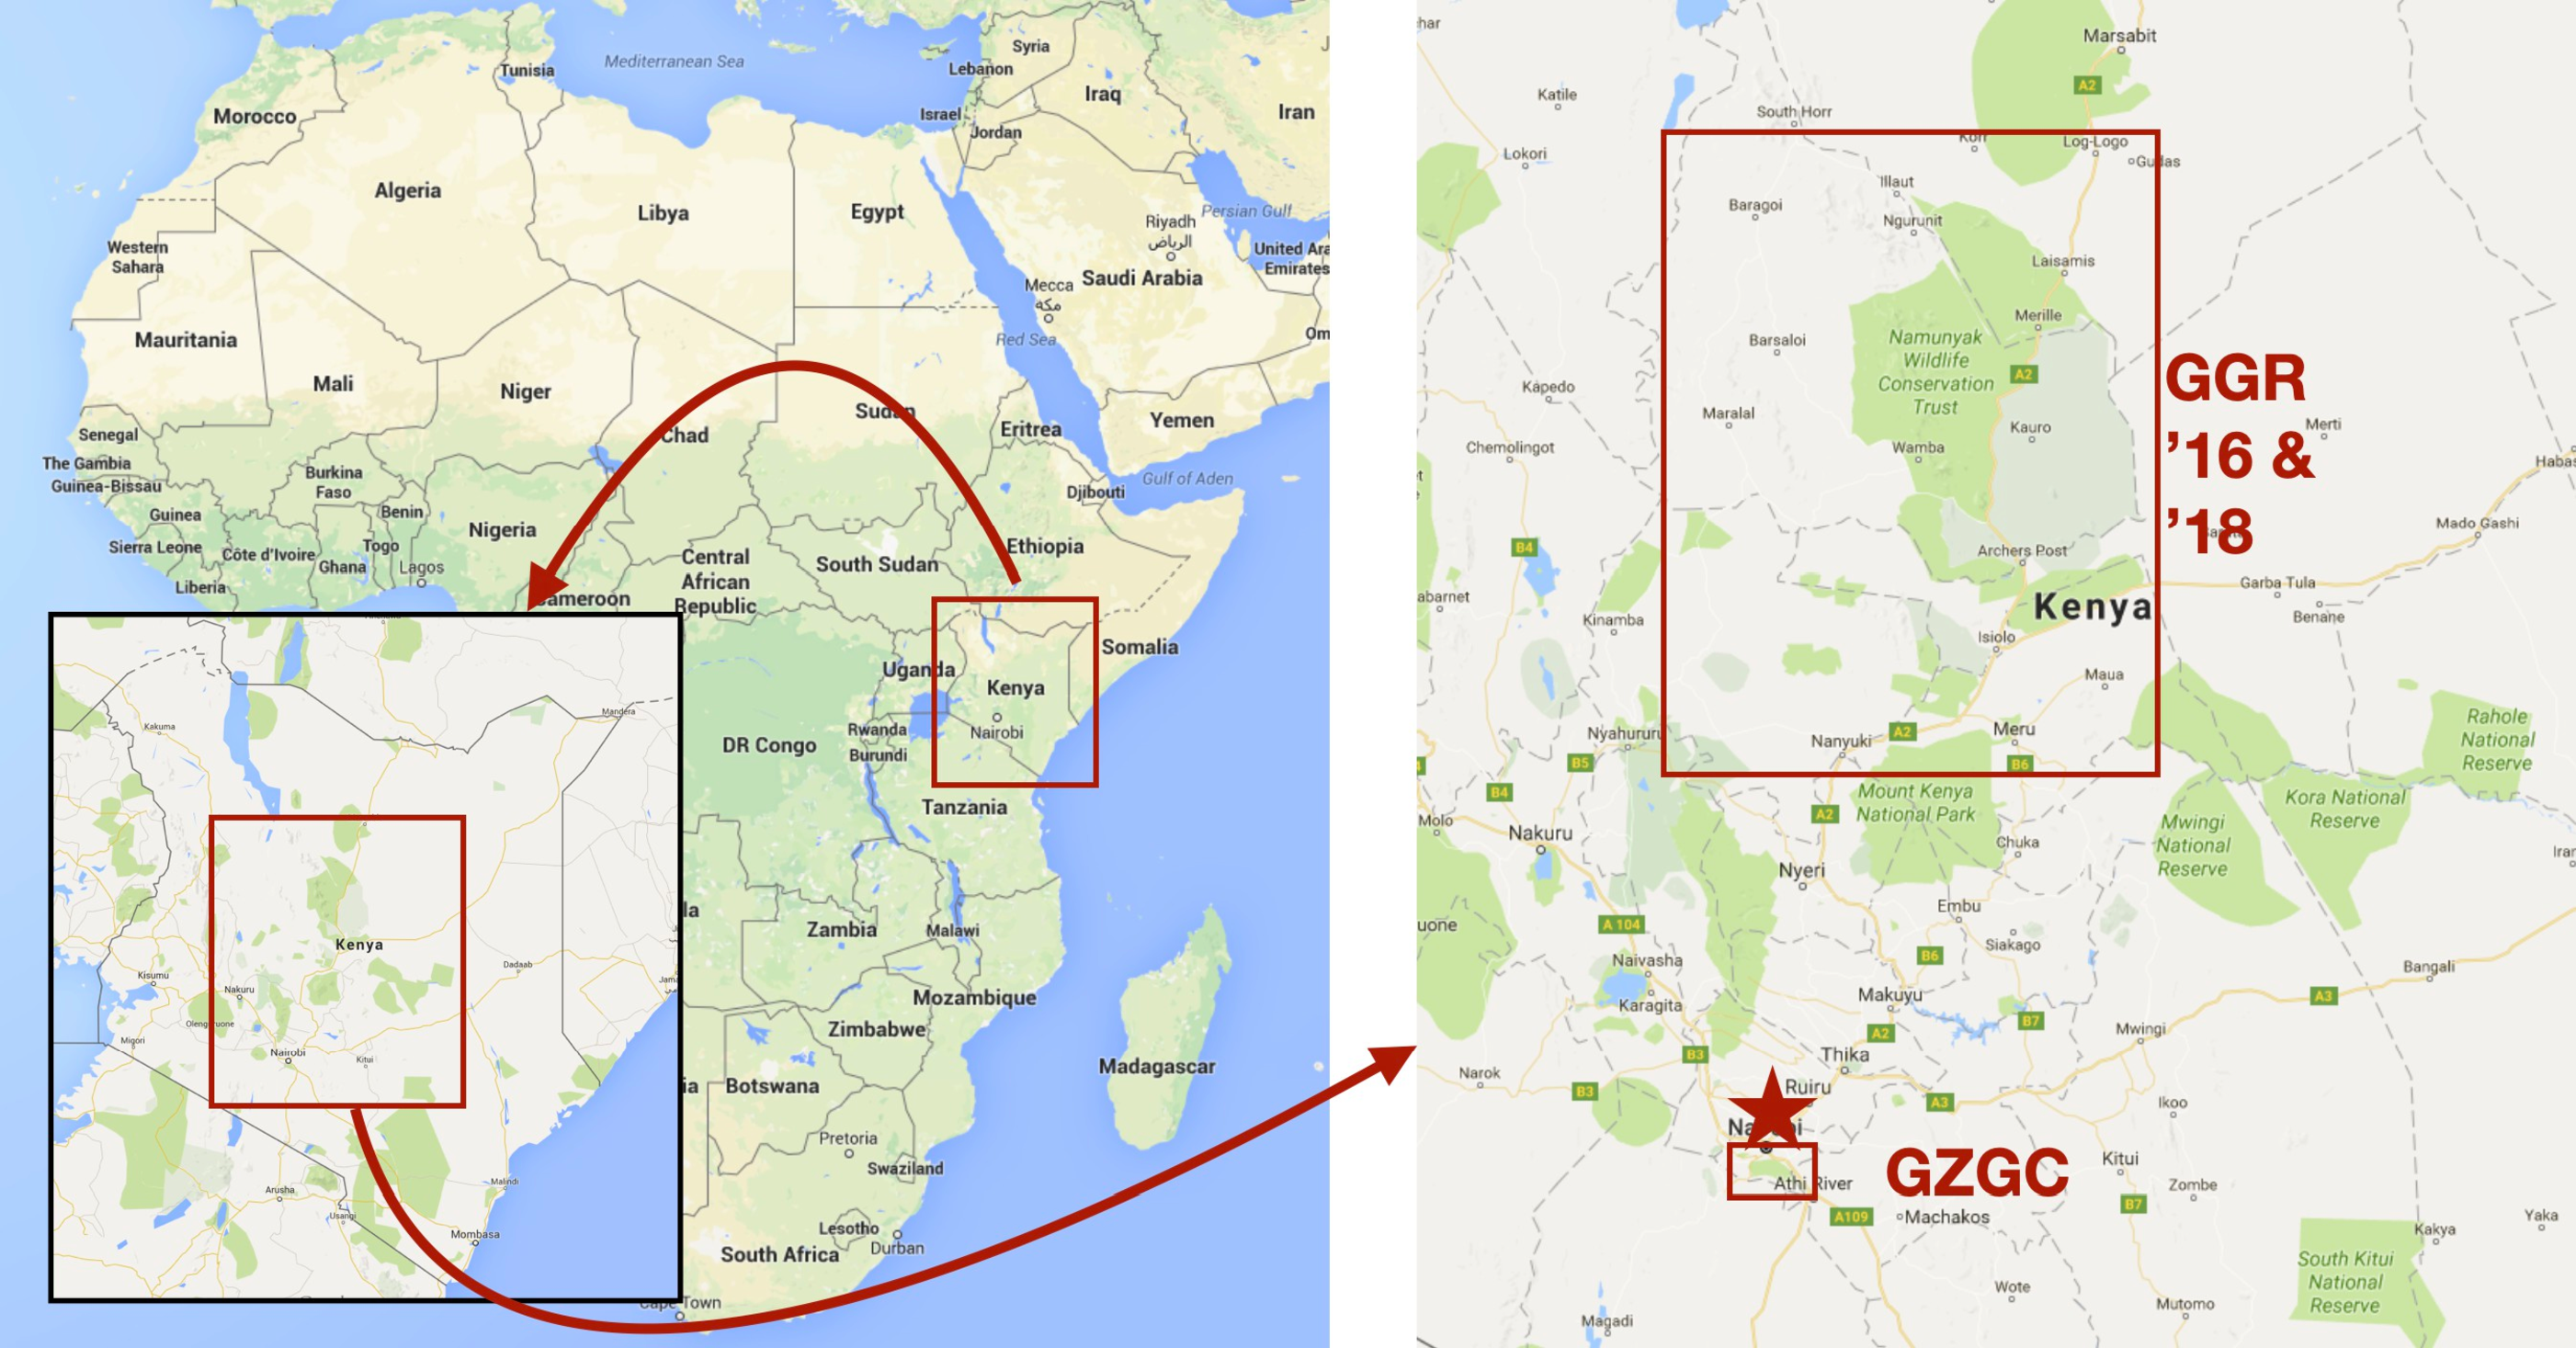
\includegraphics[width=1.0\linewidth]{resources/map-kenya.pdf}
    \end{center}
    \caption{The map of the survey boundaries for the GZGC, GGR-16, and GGR-18 photographic censusing rallies.  The survey area of the GZGC was confined to the Nairobi National Park in Nairobi, Kenya, and censused Masai giraffes and Plains zebras.  The capital city of Kenya, Nairobi, is represented with a red star.  The Great Gr\'evy's Rally 2016 and 2018 took place in the northern Laikipia region of Kenya, the primary residence area of Gr\'evy's zebra and reticulated giraffe.  Rendered with Google Maps. Best viewed in color.}
    \label{fig:maps-kenya}
\end{figure}

This chapter presents the analysis of the Great Gr\'evy's Rally (GGR), a large-scale photographic census of the entire Gr\'evy's zebra population in Kenya.  The GGR process is offered as an improved successor to the prototype process established during the Great Zebra and Giraffe Count (GZGC)~\cite{parham_photographic_2015}.  The GZGC was held March 1-2, 2015 at the Nairobi National Park in Nairobi, Kenya, and was organized to estimate the resident populations of Masai giraffes ({\em Giraffa camelopardalis tippelskirchi}) and Plains zebras ({\em Equus quagga}) within the park.  In contrast, the GGR was first held on January 30-31, 2016 in the Laikipia region of central and northern Kenya, covering the known range of Gr\'evy's zebra within the country.  The GGR was repeated on January 27-28, 2018 for the same survey area and added a second census on reticulated giraffes ({\em Giraffa reticulata}).  The reticulated giraffe population has an overlapping resident area with Gr\'evy's zebra in Kenya, making it an ideal species for simultaneous photographic censusing.  Figure~\ref{fig:maps-kenya} provides a map of Kenya and the respective survey areas for each of the three censusing rallies.  We can see that the area covered by the GGR events is much larger than the GZGC, incorporates the conservation areas of multiple Kenyan counties, and is concerned with an open animal population.

\begin{figure}[!t]
    \begin{center}
        \begin{ganttchart}[
                x unit=0.38cm,
                y unit title=0.4cm,
                y unit chart=0.47cm,
                vgrid,
                hgrid,
                title label anchor/.style={below=-1.6ex},
                title left shift=.05,
                title right shift=-.05,
                title height=1,
                bar/.style={fill=gray!50},
                incomplete/.style={fill=white},
                progress label text={},
                canvas/.append style={fill=none},
                bar height=0.7,
                group right shift=0,
                group top shift=.6,
                group height=.3,
                link bulge=.5,
            ]{1}{26}
            \gantttitle{Animal Photographic Censusing}{26} \\

            \gantttitle{Collect}{6}
            \gantttitle{Detect}{6}
            \gantttitle{Identify}{6}
            \gantttitle{Verify}{4}
            \gantttitle{Analyze}{4} \\

            \ganttgroup{Collect}{1}{6} \\
            \ganttbar{Citizen Scientist Training}{1}{2} \\
            \ganttlinkedbar{Two-Day Image Capture}{3}{5} \\
            \ganttlinkedbar{Image Aggregation}{6}{6} \\
            \ganttlinkedbar{GPS \& Time Synchronization}{6}{6} \\
            \ganttmilestone{Images Collected}{6} \\

            \ganttgroup{Detect}{7}{12} \\
            \ganttbar{Detection Ground Truth}{7}{9} \\
            \ganttbar{Whole Image Classification}{9}{9} \\
            \ganttbar{Bounding Box Regression}{9}{9} \\
            \ganttbar{Orientation Regression}{9}{9} \\
            \ganttbar{Species \& Viewpoint Labeling}{10}{10} \\
            \ganttbar{Coarse BG Segmentation}{10}{10} \\
            \ganttbar{AoI Classification}{10}{10} \\
            \ganttlinkedbar{Census Annotations}{11}{11} \\
            \ganttlinkedbar{Census Annotation Regions}{12}{12} \\
            \ganttmilestone{Detection Bootstrapped}{12} \\

            \begin{scope}[on background layer]
                \ganttlink[link type=rdldr*, link bulge 1=0.5, link mid=0.4]{elem5}{elem7}
                \ganttlink[link type=rdldr*, link bulge 1=1.5, link bulge 2=0.5, link mid=0.9]{elem8}{elem13}
                \ganttlink[link type=rdldr*, link bulge 1=1.5, link bulge 2=0.5, link mid=0.875]{elem9}{elem13}
                \ganttlink[link type=rdldr*, link bulge 2=0.5, link mid=0.833]{elem10}{elem13}
                \ganttlink[link type=rdldr*, link bulge 2=0.5, link mid=0.75]{elem11}{elem13}
                \ganttlink[link type=rdldr*, link bulge 2=0.5, link mid=0.5]{elem12}{elem13}
            \end{scope}

            \begin{scope}[on background layer]
                \ganttlink[link type=rdldr*, link bulge 2=0.5, link mid=0.5]{elem7}{elem8}
                \ganttlink[link type=rdldr*, link bulge 2=0.5, link mid=0.25]{elem7}{elem9}
                \ganttlink[link type=rdldr*, link bulge 2=1.5, link mid=0.166]{elem7}{elem10}
                \ganttlink[link type=rdldr*, link bulge 2=1.5, link mid=0.125]{elem7}{elem11}
                \ganttlink[link type=rdldr*, link bulge 2=1.5, link mid=0.10]{elem7}{elem12}
            \end{scope}

            \ganttgroup{Identify}{13}{18} \\
            \ganttbar{Photometric Checks \& Caching}{13}{13} \\
            \ganttlinkedbar{Initialize ID Database}{14}{14} \\
            \ganttlinkedbar{Human Pairwise Decisions}{14}{17} \\
            \ganttbar{Automated Verifier Decisions}{15}{17} \\
            \ganttbar{Photobomb Checks*}{15}{17} \\
            \ganttbar{Singleton Checks*}{15}{17} \\
            \ganttbar{ID Curation Cross-check*}{15}{17} \\
            \ganttbar{Animal ID Ground Truth}{17}{18} \\
            \ganttmilestone{Animal ID Database Bootstrapped}{18} \\

            \begin{scope}[on background layer]
                \ganttlink[link type=rdldr*, link bulge 1=0.5, link mid=0.4]{elem16}{elem18}
                \ganttlink[link type=rdldr*, link bulge 1=0.5, link bulge 2=0.5, link mid=0.20]{elem21}{elem20}
                \ganttlink[link type=rdldr*, link bulge 1=0.5, link bulge 2=0.5, link mid=0.10]{elem22}{elem20}
                \ganttlink[link type=rdldr*, link bulge 1=0.5, link bulge 2=0.5, link mid=0.0666]{elem23}{elem20}
                \ganttlink[link type=rdldr*, link bulge 1=0.5, link bulge 2=0.5, link mid=0.05]{elem24}{elem20}

                \ganttlink[link type=rdldr*, link bulge 1=0.5, link bulge 2=0.5, link mid=0.50]{elem20}{elem21}
                \ganttlink[link type=rdldr*, link bulge 1=0.5, link bulge 2=0.5, link mid=0.25]{elem20}{elem22}
                \ganttlink[link type=rdldr*, link bulge 1=0.5, link bulge 2=0.5, link mid=0.166]{elem20}{elem23}
                \ganttlink[link type=rdldr*, link bulge 1=0.5, link bulge 2=0.5, link mid=0.125]{elem20}{elem24}
                \ganttlink[link type=rdldr*, link bulge 1=0.5, link bulge 2=2.5, link mid=0.1]{elem20}{elem25}
            \end{scope}

            \ganttgroup{Verify}{19}{22} \\
            \ganttbar{Demographic Ground Truth}{19}{20} \\
            \ganttbar{Gender Consistency Checks}{21}{22} \\
            \ganttbar{Speed Quality Checks}{21}{22} \\
            \ganttmilestone{Ecology Bootstrapped}{22} \\

            \begin{scope}[on background layer]
                \ganttlink[link type=rdldr*, link bulge 1=0.5, link mid=0.4]{elem26}{elem28}
                \ganttlink[link type=rdldr*, link bulge 1=0.5, link bulge 2=2.5,link mid=0.27]{elem26}{elem29}
                \ganttlink[link type=rdldr*, link bulge 1=0.5,link bulge 2=0.5, link mid=0.21]{elem26}{elem30}
            \end{scope}

            \ganttgroup{Analyze}{23}{26} \\
            \ganttbar{Petersen-Lincoln Index}{23}{24} \\
            \ganttbar{Participant Effectiveness}{23}{24} \\
            \ganttbar{Geographical Coverage}{23}{24} \\
            \ganttbar{Local/National Comparisons}{23}{24} \\
            \ganttbar{Historical Comparisons}{25}{26} \\
            \ganttmilestone{Current Population Estimate}{26}

            \begin{scope}[on background layer]
                \ganttlink[link type=rdldr*, link bulge 1=0.5, link mid=0.4]{elem31}{elem33}
                \ganttlink[link type=rdldr*, link bulge 1=0.5, link mid=0.27]{elem31}{elem34}
                \ganttlink[link type=rdldr*, link bulge 1=0.5, link mid=0.21]{elem31}{elem35}
                \ganttlink[link type=rdldr*, link bulge 1=0.5, link mid=0.166]{elem31}{elem36}
                \ganttlink[link type=rdldr*, link bulge 2=2.5, link bulge 1=0.5, link mid=0.14]{elem31}{elem37}
            \end{scope}
        \end{ganttchart}
    \end{center}
    \caption{A Gantt chart for the recommended process used for animal photographic censusing, including data collection and boostrapping of the detection pipeline for novel species.  *Steps were not used during the GGR-16 and GGR-18.}
    \label{fig:gantt}
\end{figure}

The GGR events in 2016 and 2018 (referred to as ``GGR-16'' and ``GGR-18'', respectively) significantly refined the photographic censusing process used during the GZGC. Both GGR-16 and GGR-18 sampled a significantly larger geographical area, produced more confident population estimates than historical estimates, and massively increased the amount of automation with better computer vision algorithms.  Across the three censusing rallies, approximately 100,000 photographs were processed and collected by more than 400 volunteer citizen scientists, including biologists, park rangers, computer programmers, tourists, and school children. As a result, the GGR is the largest known photographic census of Gr\'evy's zebra ever performed and is estimated to have cataloged 70\% of all Gr\'evy's zebra in Kenya (as we will see later), representing the most accurate and comprehensive census of the species to date.  Furthermore, the Gr\'evy's zebra population estimates from the GGR-18 have been accepted by the Kenyan government as the country's official population count. This recognition has never before been granted to a non-governmental group.

In summary, this chapter has two goals.  The first is to describe the procedures of the GGR data collection events and processing, contrasting them with the earlier GZGC event.  This process includes using the detection pipeline (without Census Annotations) and the Graph ID animal ID curation algorithm to build an ID database, which was the current state of the analysis at the time in 2016 and 2018.  As described below, this database is checked with various automated tools and human decisions for redundancy and subjected to quality checks to ensure accuracy.  Furthermore, the final population estimates for both rallies are generated after extensive human effort because, as stated, some of the automation tools presented earlier in this dissertation were unavailable at the time.  The second goal of this chapter is to re-analyze the GGR-18 event using these new tools.  This new analysis is a culminating experiment to show the effectiveness of the methods developed (CA and CA-R) or incorporated (LCA) to reduce human interaction while maintaining a consistent population estimate.  The updated mathematical framework (see Section~\ref{sec:ca-math}) is also used for the first time to fine-tune the final population estimate after taking into account the overall estimated effect of the machine learning algorithm's errors.

\section{The Great Gr\'evy's Rally (GGR) in 2016 and 2018}

\begin{table}[!t]
    \caption{The number of cars, cameras, and photographs for the GZCD, GGR-16, and GGR-18 photographic censusing rallies.  The GGR rallies had over three times as many citizen scientists who contributed four times the number of photographs for processing.  The GGR-18 rally, as compared to GGR-16, included a 33\% increase in photographers and a 21\% increase in the number of photographs collected. [GZGC \& GGR-16] \copyright 2017 AAAI. Reprinted, with permission, from: J. Parham, J. Crall, C. Stewart, T. Berger-Wolf, and D. I. Rubenstein, ``Animal population censusing at scale with citizen science and photographic identification,'' in \textit{AAAI Spring Symp.}, Palo Alto, CA, USA, Jan. 2017, pp. 37–44. [GGR-16 \& GGR-18] \copyright 2018 IJCAI. Reprinted, with permission, from: J. Parham, C. Stewart, T. Berger-Wolf, D. Rubenstein, and J. Holmberg, ``The Great Grevy’s Rally: A review on procedure,'' in \textit{AI Wildlife Conserv. Workshop}, Stockholm, Sweden, Jul. 2018, pp.1–3.}
    \label{table:collection}
    \begin{center}
        \begin{tabular}{| l | r | r | r |}
            \hline
                   & Cars & Cameras & Photographs \\
            \hline
            GZGC   & 27   & 55      & 9,406       \\
            \hline
            GGR-16 & 121  & 162     & 40,810      \\
            \hline
            GGR-18 & 143  & 214     & 49,526      \\
            \hline
        \end{tabular}
    \end{center}
\end{table}

Both Great Gr\'evy's Rally censusing events followed the same procedure, presented as a complete process flow diagram in Figure~\ref{fig:gantt}.  One of the primary benefits is that all of the machine learning components can be bootstrapped as the analysis proceeds with the help of human annotators.  This design is crucial as ready-to-go, pre-existing machine learning models are not available for most endangered species. Furthermore, once the machine learning components are successfully trained, they can be reused for future events with the same collection procedure and species of interest.  This section provides details for how images were collected and aggregated for processing during the GGR events and describes how the detection pipeline was applied on real-world imagery. First, images collected from citizen scientists need to be aggregated and synchronized for accurate GPS and time metadata.  Next, the resulting annotations must be curated into an animal ID database with ranking and verification algorithms.  The following discussion explains how the GGR-16 and GGR-18 events created their respective ID databases, which were subject to different automated algorithm versions at the time.  Lastly, after consistency checks, the population estimates for Gr\'evy's zebra and reticulated giraffes are reported.

\subsection{Image Collection with Citizen Scientists}

A vital feature of the censusing procedure is the ability to distribute and parallelize the collection of animal imagery.  The robustness of the sight-resight study critically depends on capturing as many sightings and resightings of individuals.  This design is in sharp contrast to a count-based estimate which must always be careful to avoid double counting and overlapping sample regions.  Additional advantages of using cameras during a census include 1) it provides actionable evidence of where a specific individual was in time and location (which allows for the possibility of future auditing) and 2) the mechanism is easy to teach to the average person. Furthermore, by not requiring specialized hardware -- only a car and a GPS-enabled camera -- a large area can be surveyed efficiently, with many photographers overlapping the same geographical area at the same time. Another essential feature of the data collection is its cost-effectiveness, as citizen scientists, volunteers, tourists, field guides, school children, park rangers, scientists, and any other stationary ground-based sources (e.g., camera traps) can all volunteer to contribute data.

\begin{figure}[!t]
    \begin{center}
        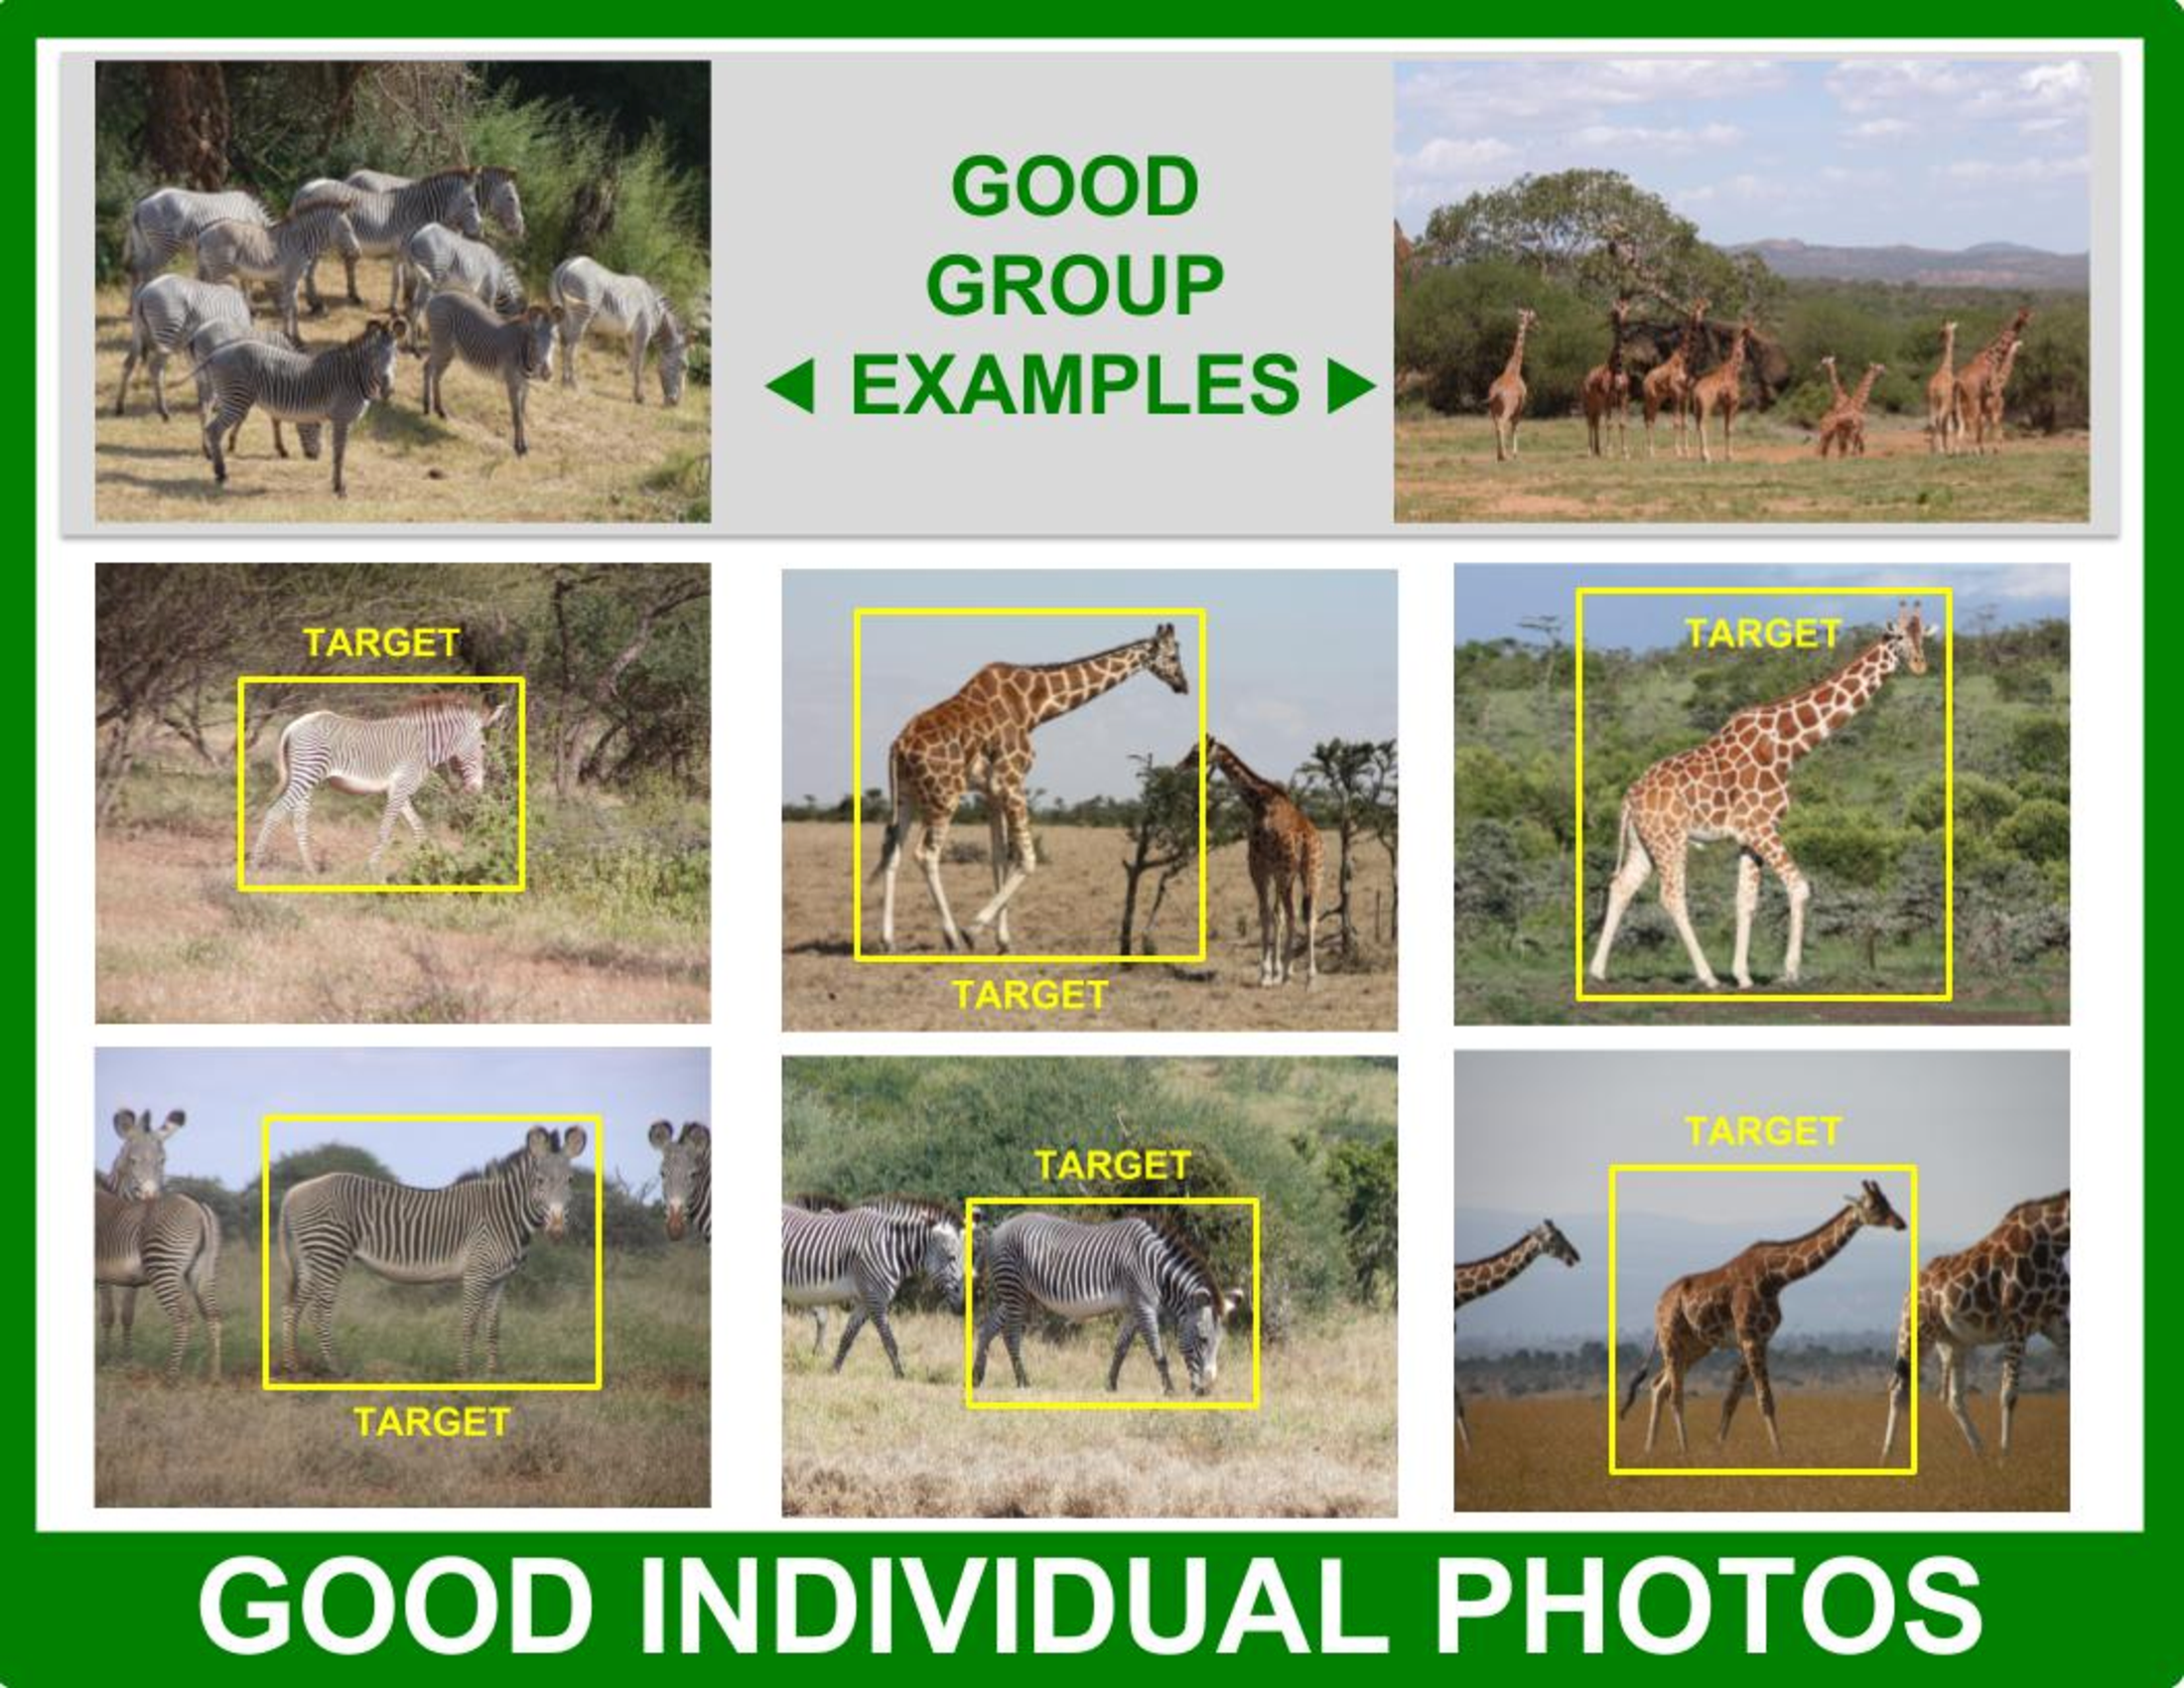
\includegraphics[width=0.72\linewidth]{resources/training-good-new.pdf} \\
        \vspace{3mm}
        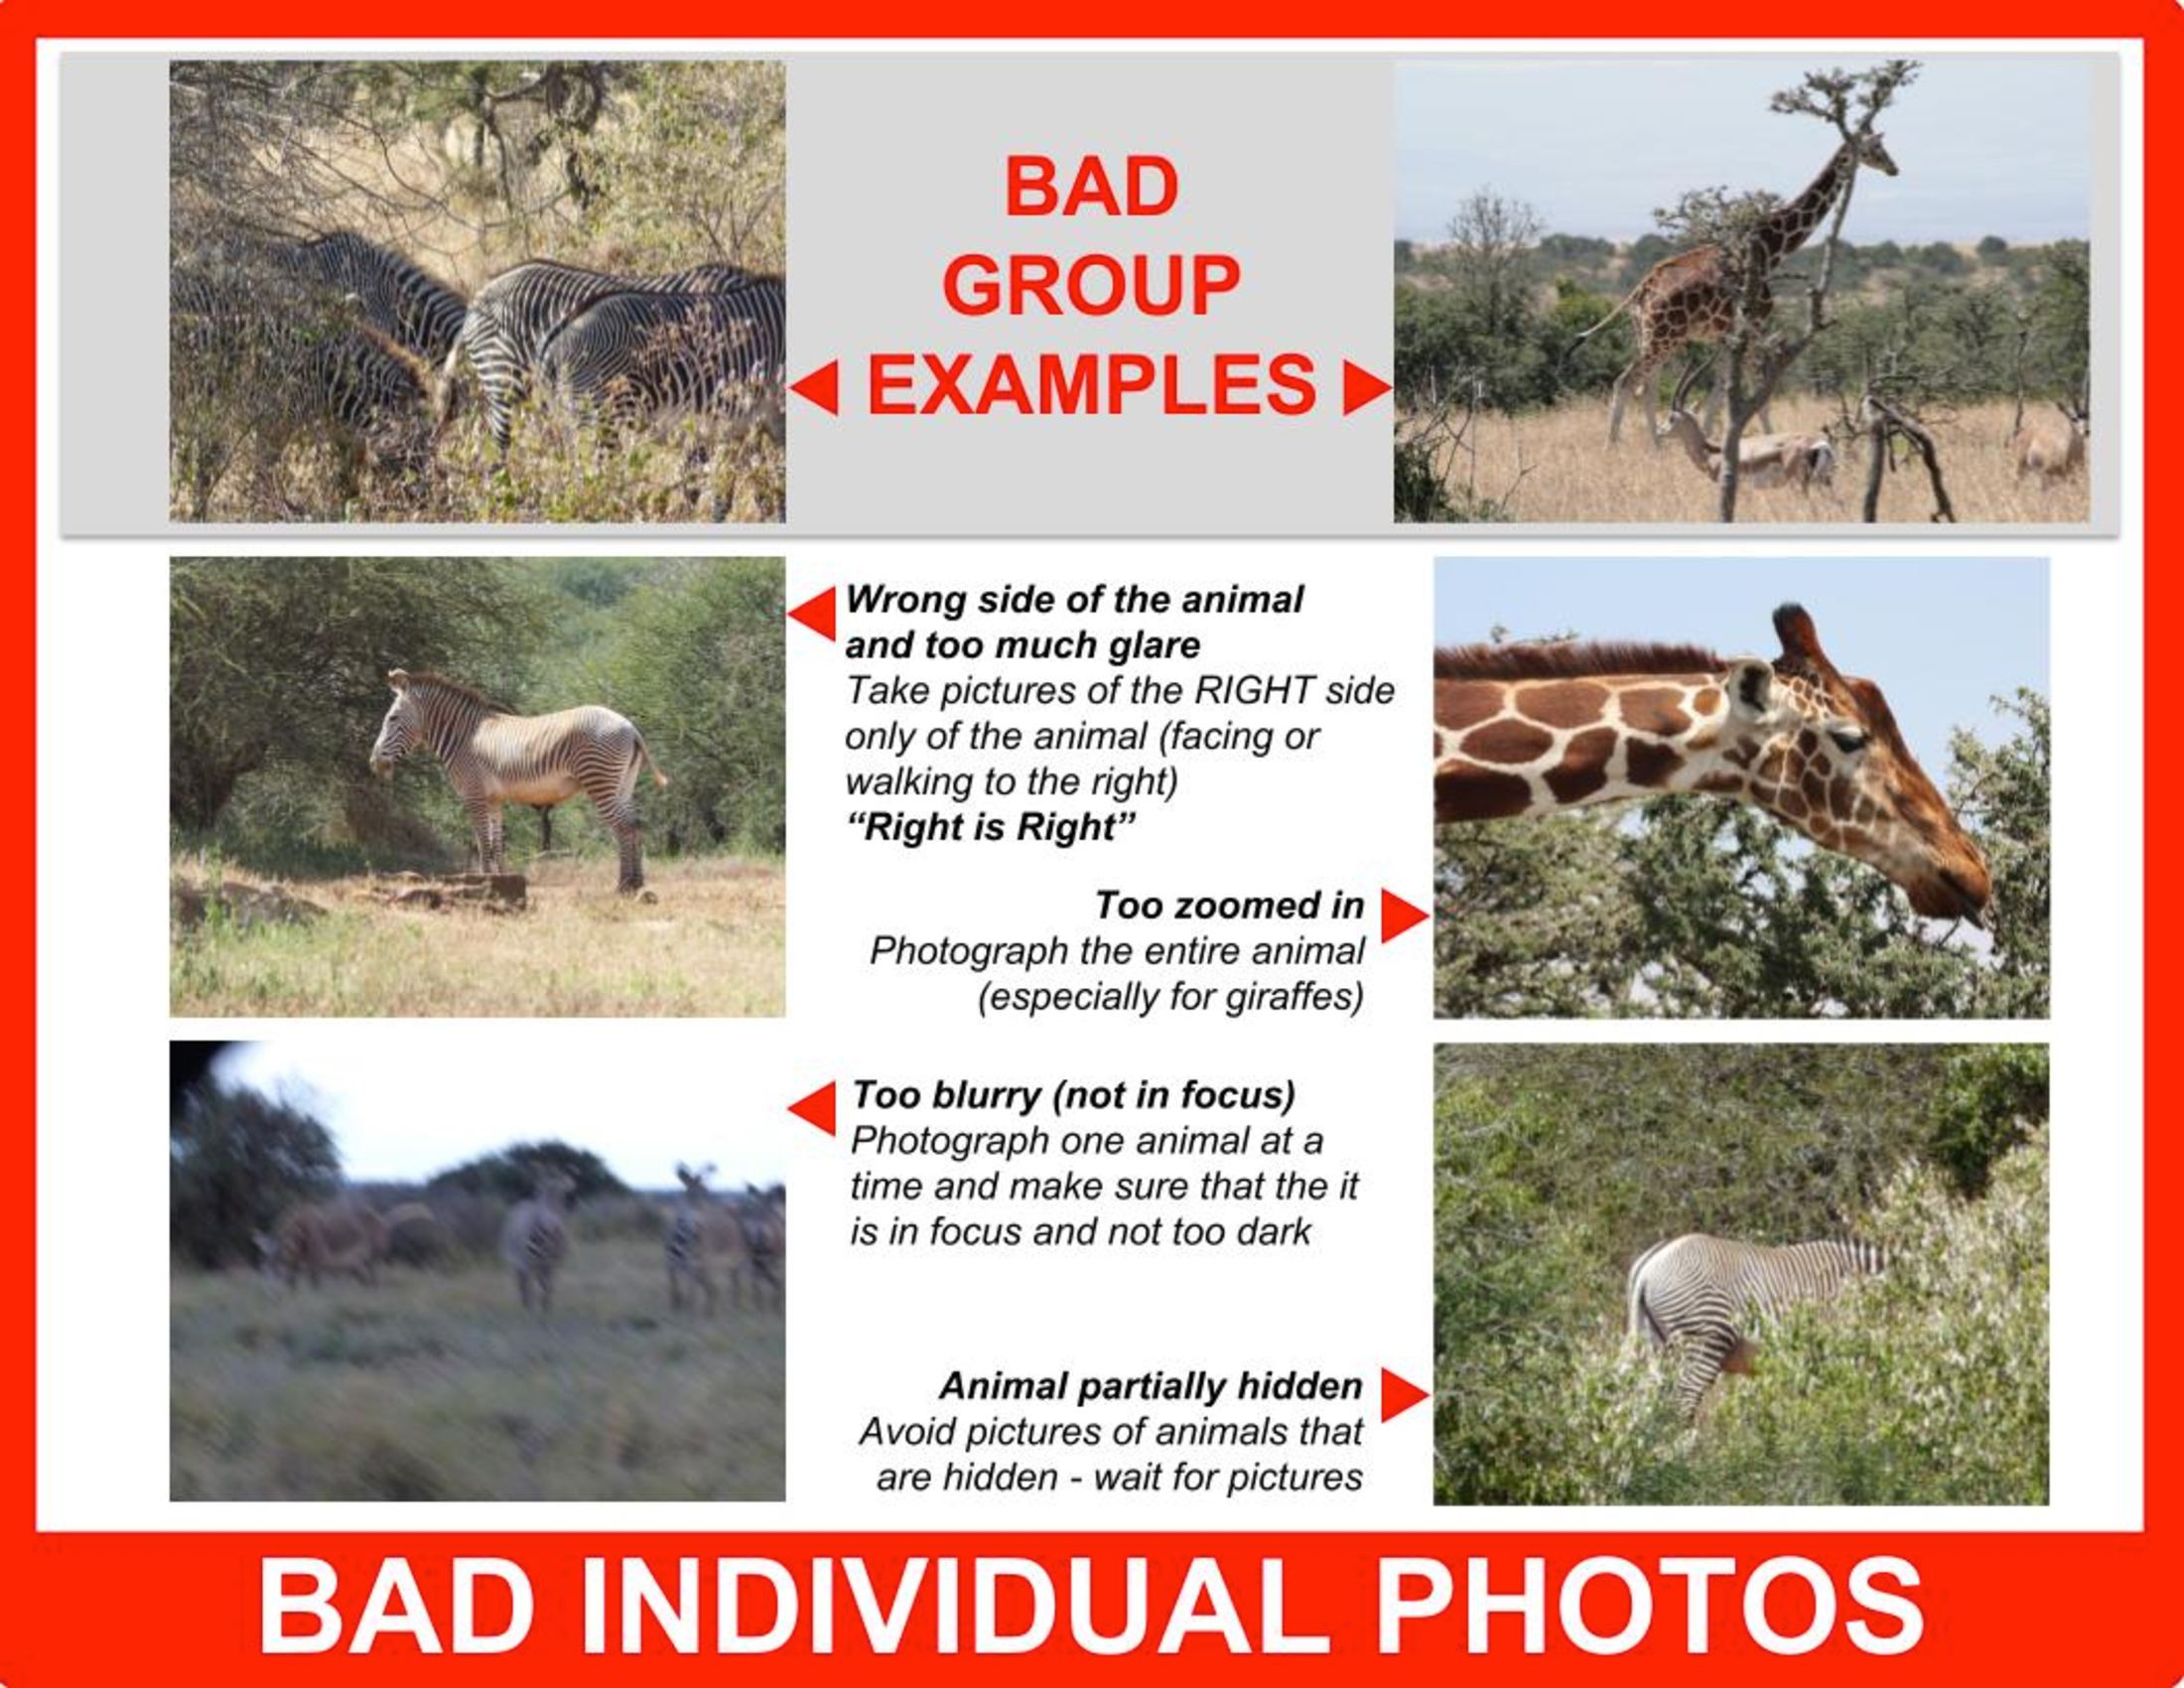
\includegraphics[width=0.72\linewidth]{resources/training-bad-new.pdf}
    \end{center}
    \caption{An image of the participant training ``cheat sheet'' used during the GGR-18 photographic censusing rally, showing the \textit{do's} and \textit{don'ts} for capturing images.  The examples are explicitly updated to bias the participants towards taking better pictures of AoIs, even showing a primary \textit{target} on the good examples.}
    \label{fig:cheatsheet}
\end{figure}

The number of cars and volunteers, and the number of photographs taken for the three rallies, are summarized in Table~\ref{table:collection}.  Since the volunteers taking photographs are \textit{mobile}, they can go where the animals are; this is in stark contrast to data capture that uses only static camera traps or fixed-route surveys.  It is worth noting that the number of images collected during the GGR-18 is 20\% higher and with 30\% more photographers compared to the GGR-16 event.  Furthermore, it was recognized that the volunteer photographers for all three censusing events did not expect to be paid for their effort.  In other words, there seemed to be an intrinsic worth for participants to be part of a scientific endeavor, which was enough compensation in itself.  This fortuitous effect suggests that photographic censusing is an effective method of community engagement.\footnote{Refer to~\cite{parham_photographic_2015} for an example on how to reward volunteer citizen scientist participants for their time and image contributions.  For GZGC, a same-day print-out was provided to each participant that listed known and new animals they photographed.}  The GGR-18 event was able to recruit photographers that participated in the GGR-16 event, exemplifying the fact that some participants were willing to volunteer their time without the need for incentives from the organizers.  Before we delve deeper into the analysis of the collected images, let us review the participants' training procedure that was provided prior to each event.

\subsubsection{Citizen Scientist Training}

The participating photographers were asked to go into an assigned survey area via car and capture images of the species of interest (i.e., Gr\'evy's zebra and reticulated giraffe).  Prior to departing, each participant was given a training document and a Cheat Sheet (Figure~\ref{fig:cheatsheet}) that showed the common \textit{do's} and \textit{don'ts} of a photographic collection.  For example, the participant training document given to participants of the GGR-18 is provided in Appendix A, and it includes instructions on how to set up the Nikon GPS-enabled cameras.  The participant instructions were updated slightly between the GZGC, GGR-16, and GGR-18 censusing events based on a better understanding of how the detection pipeline and ID systems were failing.  The training process created a feedback loop, where subtle differences in the training instructions influenced the quality of images collected.  For example, the GGR-18 training instructions encouraged the photographer to:

\numsquishlist
\item Pick a single subject (of the target species and target viewpoint),
\item Always take a picture of an animal in the foreground,
\item Place the subject in the center of the photograph, and
\item Zoom the camera such that the animal covers around 50\% of the image (if possible).
\numsquishend

All photographers for the GZGC were requested to take pictures of the left sides of plains zebras and Masai giraffes, while photographers for the GGR were requested to take pictures of the right sides of Gr\'evy's zebras and reticulated giraffes.  Having a consistent viewpoint (left or right) allows for more effective sight-resight and reduces the chance of ML errors. Furthermore, the distinguishing visual markings for these species are not left-right symmetrical, so the animal's appearance differs (sometimes significantly) from side to side.  This asymmetry means that a right-only census must discard a left viewpoint sighting as irrelevant data.

Along with guidance on species, photographers were shown examples of good/poor quality photographs emphasizing 1) the correct side of the animal, 2) getting a large enough and clear view, and 3) seeing the animal in relative isolation from other animals.  To better guarantee a valuable sighting, GGR photographers were requested to take about three pictures of the right side of each Gr\'evy's zebra they saw.  In both the GZGC and GGR, photographers were invited to take other pictures once they had adequately photographed each encountered animal, causing miscellaneous photographs to be collected.  This decision was primarily to help minimize photographer fatigue and allow flexibility when an exciting or otherwise rare species was encountered.

In contrast, the instructions for the GGR-16 did not focus on a target animal, only emphasizing the correct species and viewpoint.  The above changes nudged the photographers during the GGR to take better pictures of animals by implicitly focusing on the concepts that overlap with Annotation of Interest (AoI, see Section~\ref{sec:aoi}).  To make the \textit{a priori} decision more straightforward for the AoI detection component, specific examples and instructions to guide participants into taking better images were provided.  Furthermore, the concept of a Census Annotation did not exist when the GGR-16 or GGR-18 collections were performed.  However, the benefit of asking photographers to focus on features consistent with AoIs is that it also biased the participant to capture good CA examples.  We saw in Section~\ref{sec:ca-aoi-compare} a strong correlation between AoI and CA, indicating that the collected animal sightings were still strongly biased towards identifiability.

\subsubsection{GPS Cameras \& Time Synchronization}

\begin{figure}[!t]
    \begin{center}
        \includegraphics[width=0.8\linewidth]{resources/2.pdf}
    \end{center}
    \caption{An image of the camera card used for the GGR-18 participant ``photographer 1'' who was assigned to ``car 1''.  A QR detection algorithm  was used to automatically localize the first photograph that was used to sync all participants in a car.}
    \label{fig:card}
\end{figure}

Upon registering for the GGR-18 censusing rally, all participants were given a GPS-enabled camera and a paper ``camera card''.  This procedure is similar to the GZGC, except for how GPS locations were synchronized across cars.  During the GZGC, a dedicated GPS dongle was provided for each car, and participants could bring their cameras. Unfortunately, this open policy proved to be a synchronization challenge across multiple timestamp formats, failures to start GPS recording, and other miscellaneous inconsistencies or problems. As a result, the GGR-16 and GGR-18 procedures were improved to address these issues:

\begin{enumerate}
    \item A Nikon GPS-enabled camera was provided to every car that volunteered to take pictures for the rally.  This camera is always labeled with the letter ``A'' within the car. In addition, a GPS camera replaced the GPS dongle that was provided to every car during the GZGC.  All photographers' times of their photographs were assigned locations via a look-up table from the GPS log.
    \item A QR code was added to the camera card that provided a link to the Great Gr\'evy's Rally website\footnote{\url{greatgrevysrally.com} (Accessed: Oct. 29, 2021).}, which also embedded the car number and photographer letter into the URL.
    \item The ``3-2-1 Snap'' handout used during the GZGC\footnote{See Section 2.1 of~\cite{parham_photographic_2015}, mentioned there as a photographer's $Image_0$.} was combined and consolidated with the camera cards.  The for GZGC, all participants in a car used a physical sheet of paper to take a synchronized photograph at the start of the day.  Each participant then wrote the local time for when the picture was taken on their registration cards.  The written time, the photograph, and the camera's internal clock were used to calculate the correct time for each image a photographer contributed.  For the GGR-16 and GGR-18, the ``3-2-1 Snap'' wording was added to the front side of the camera card, which was used to coordinate all photographers in a car.  Since at least one camera in the car was guaranteed to support GPS (and therefore has access to accurate timestamps), participants did not need to write down the local time.
\end{enumerate}

\noindent An example sync image of the camera card with QR code can be seen in Figure~\ref{fig:card}.  During processing, the images were automatically scanned to find the QR code for each photographer in a car.  The timestamps of the QR code are associated with the correct timestamp provided by the GPS camera, which receives accurate date and time data from the orbiting satellites.  A given photographer's images were then assigned a ``timedelta'' (i.e., a time offset), which was used to correct their respective EXIF timestamps to local Kenya time.  Furthermore, there is a unique QR code for day 1 and day 2 of the census rally.  The second QR code and ``3-2-1 Snap'' image are used to cross-reference and check the \textit{timedelta} calculation for a given photographer.  The benefit of using a separate QR code for days 1 and 2 is that it adds redundancy because some photographers forgot to take the image on either day.  In that event, the assumption is that the system clock of each participant's camera is at least internally consistent, so one timestamp is sufficient to establish the correction factor.

\subsubsection{Aggregating Multiple Cameras}

\begin{figure}[!t]
    \begin{center}
        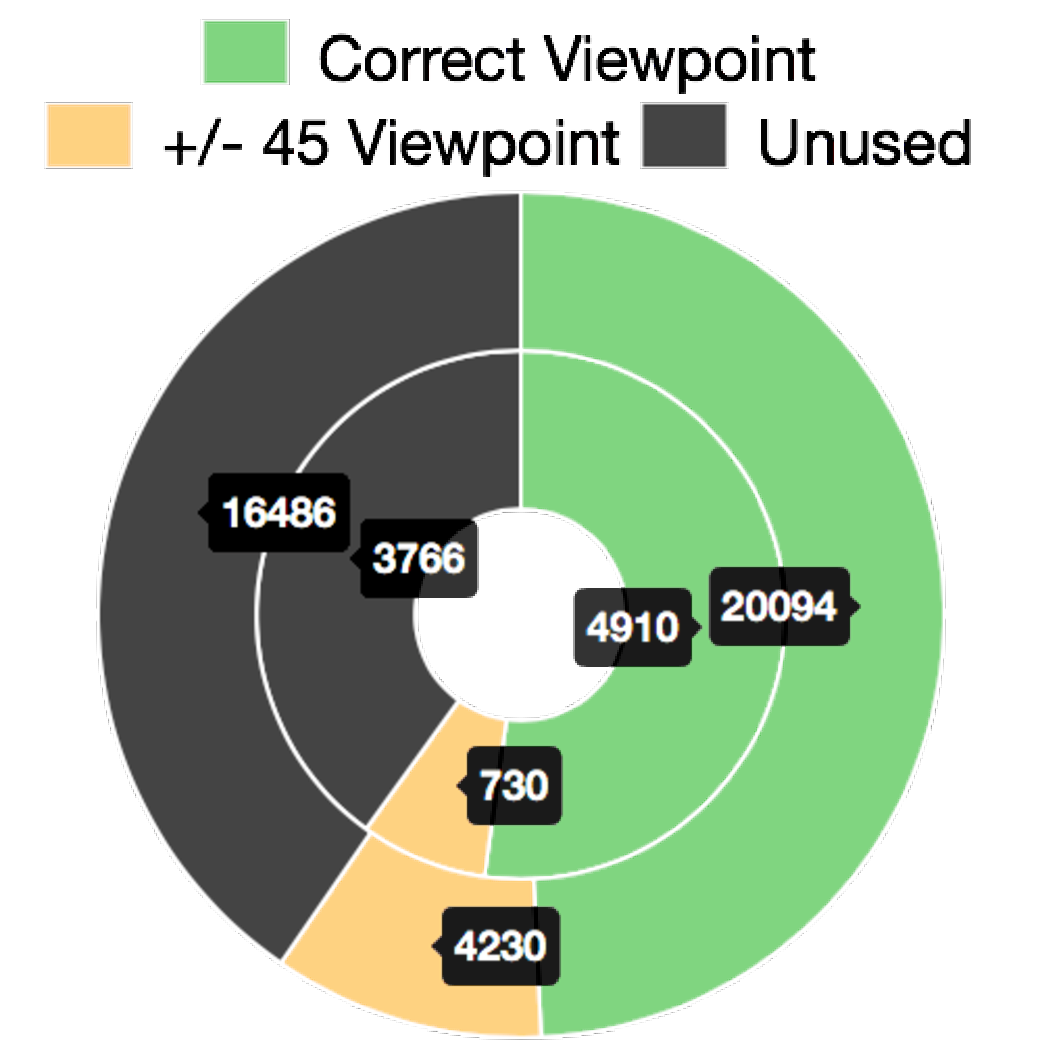
\includegraphics[width=0.48\linewidth]{resources/images-used-viewpoint.pdf}
        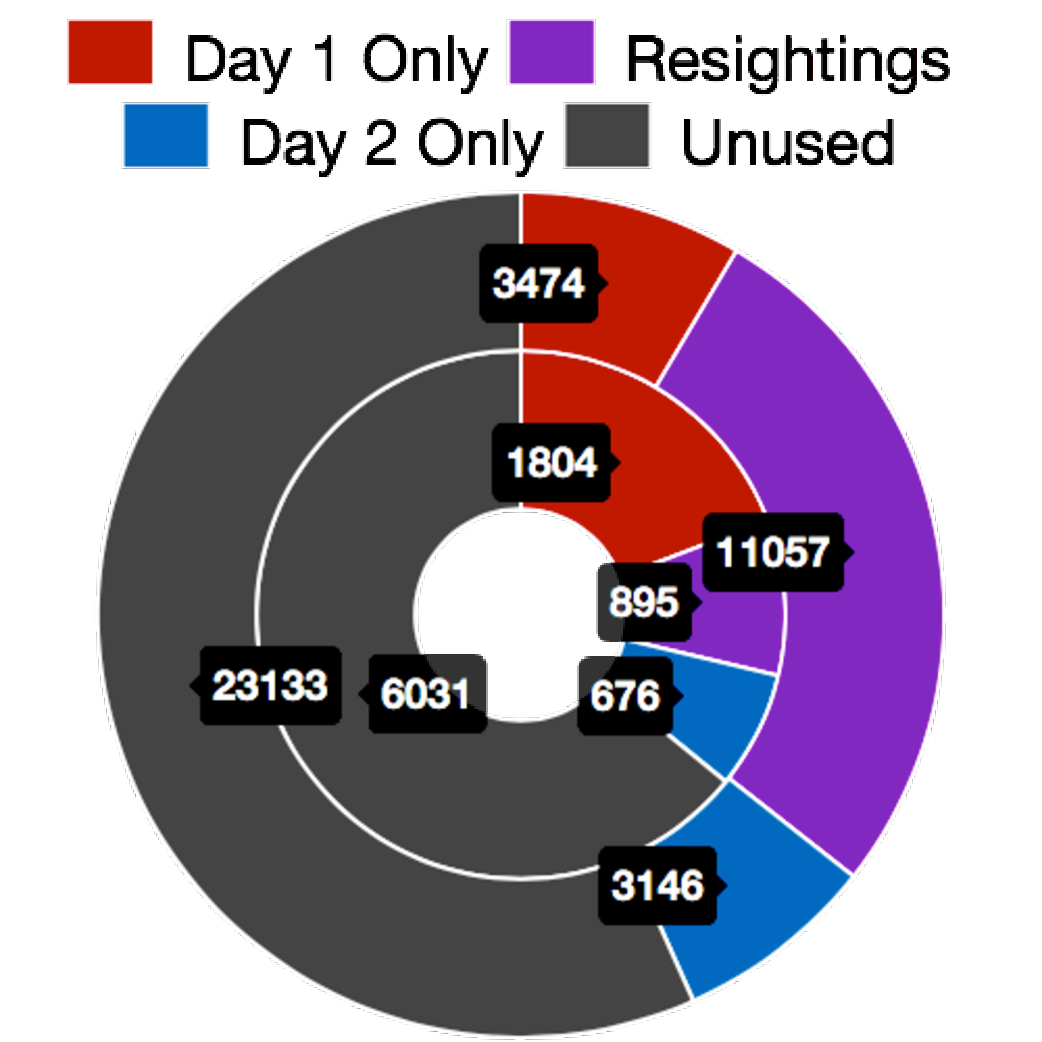
\includegraphics[width=0.48\linewidth]{resources/images-used-resights-all.pdf}
    \end{center}
    \caption{The number of photographs (left) that adhered to the collection protocol for the GZGC (inner-ring) and the GGR-16 (outer-ring).  The number of photographs that adhered to the viewpoint collection protocol was around 50\% (green) for the GGR-16 and the GZGC.  The number of which photographs (right) that had sightings on day 1 only, day 2 only, and resightings for the GZGC (inner-ring) and GGR-16 (outer-ring); the sightings data and its colors are meant to mirror that of Figure~\ref{fig:maps-gzgc}.  Note that any photographs with no sightings are grouped with unused.  \copyright 2017 AAAI. Reprinted, with permission, from: J. Parham, J. Crall, C. Stewart, T. Berger-Wolf, and D. I. Rubenstein, ``Animal population censusing at scale with citizen science and photographic identification,'' in \textit{AAAI Spring Symp.}, Palo Alto, CA, USA, Jan. 2017, pp. 37–44.}
    \label{fig:breakdown}
\end{figure}

After the photographers took the images, censusing rally staff collected and stored them onto a single centralized computer.  Each photographer's camera card was used to create a named folder of that participant's images during collection (e.g., ``GGR-18/CAR-1/CAMERA-A'').  The photographers within the same car had the same car number, each with their own unique camera letter.  The letter ``A'' was reserved for the census-provided GPS-enabled camera in the car taking photographs.  Unfortunately, this relatively simple procedure still resulted in the inappropriate images being grouped -- the approximately 250GB of collected data during each event needed to be cleaned and restructured.

The QR detection algorithm searched a photographer's contributed images to find the \textit{first} image that had a QR code.  Some data organizing errors were found by comparing the QR camera card photograph (which embeds photographer information) with its assigned folder name.  For example, with the GGR-18 data, 45 manual resolutions needed to be made, including renaming folders, merging two folders, and moving folders from one car to another.  The first QR image of the rally was assumed to have been taken simultaneously with the A camera, providing a method to establish the non-A camera's time offset from local time and approximate GPS location.  However, the QR code detection was not perfect.  Sometimes a human reviewer had to manually search for the QR code by hand, starting with the photographer's earliest images working forwards in time.  Images taken outside of the time range of the two-day event were discarded to preserve the privacy of the contributors.  For example, the data collected during the GGR-18 had 53,193 images, but 3,649 were taken outside the two-day time window or geofence boundary of the censusing rally.

\begin{figure}[!t]
    \begin{center}
        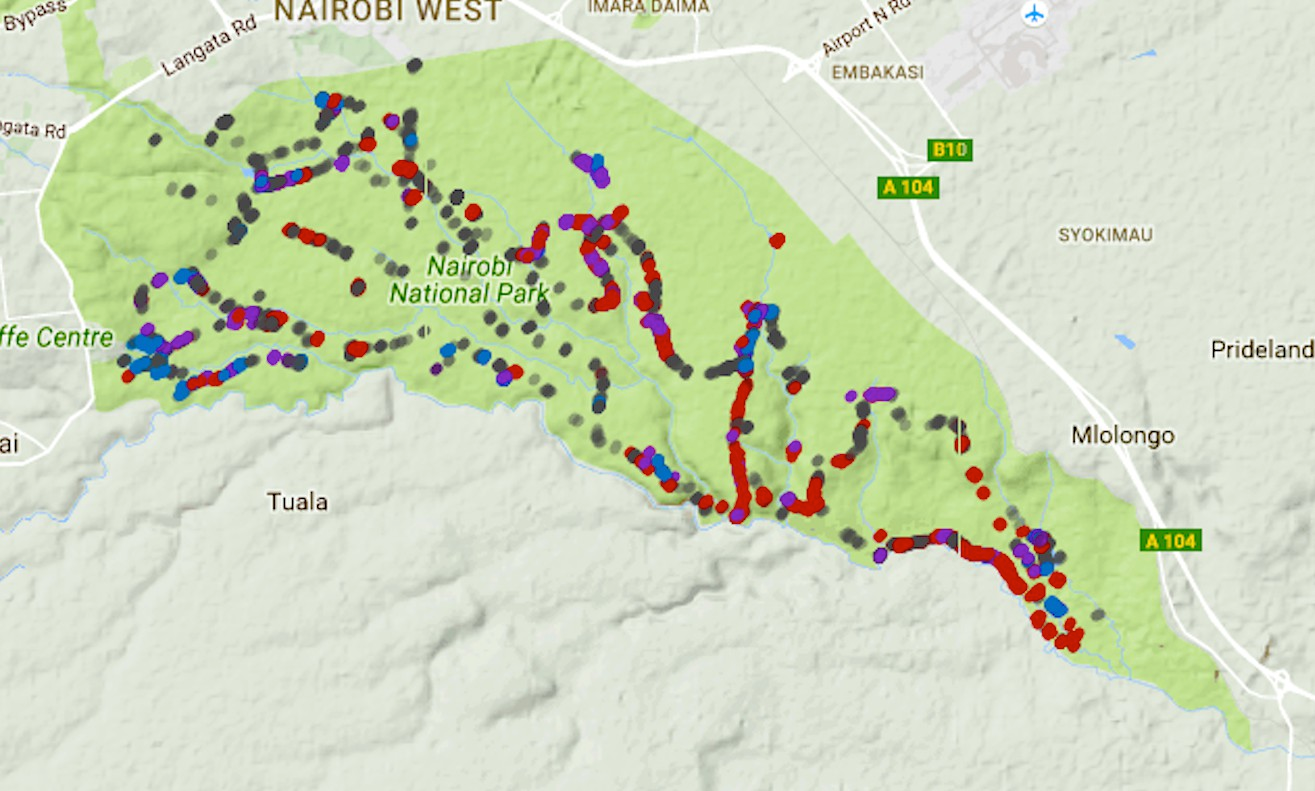
\includegraphics[width=0.9\linewidth]{resources/map-gzgc-all.pdf}
    \end{center}
    \caption{The map of image GPS locations from the GZGC censusing rally.  Colored dots indicate sightings during the two days of each census; red was from day 1 only, blue was day 2 only, purple was resightings, and gray were unused.  Rendered with Google Maps. Best viewed in color.  \copyright 2017 AAAI. Reprinted, with permission, from: J. Parham, J. Crall, C. Stewart, T. Berger-Wolf, and D. I. Rubenstein, ``Animal population censusing at scale with citizen science and photographic identification,'' in \textit{AAAI Spring Symp.}, Palo Alto, CA, USA, Jan. 2017, pp. 37–44.}
    \label{fig:maps-gzgc}
\end{figure}

\begin{figure}[!t]
    \begin{center}
        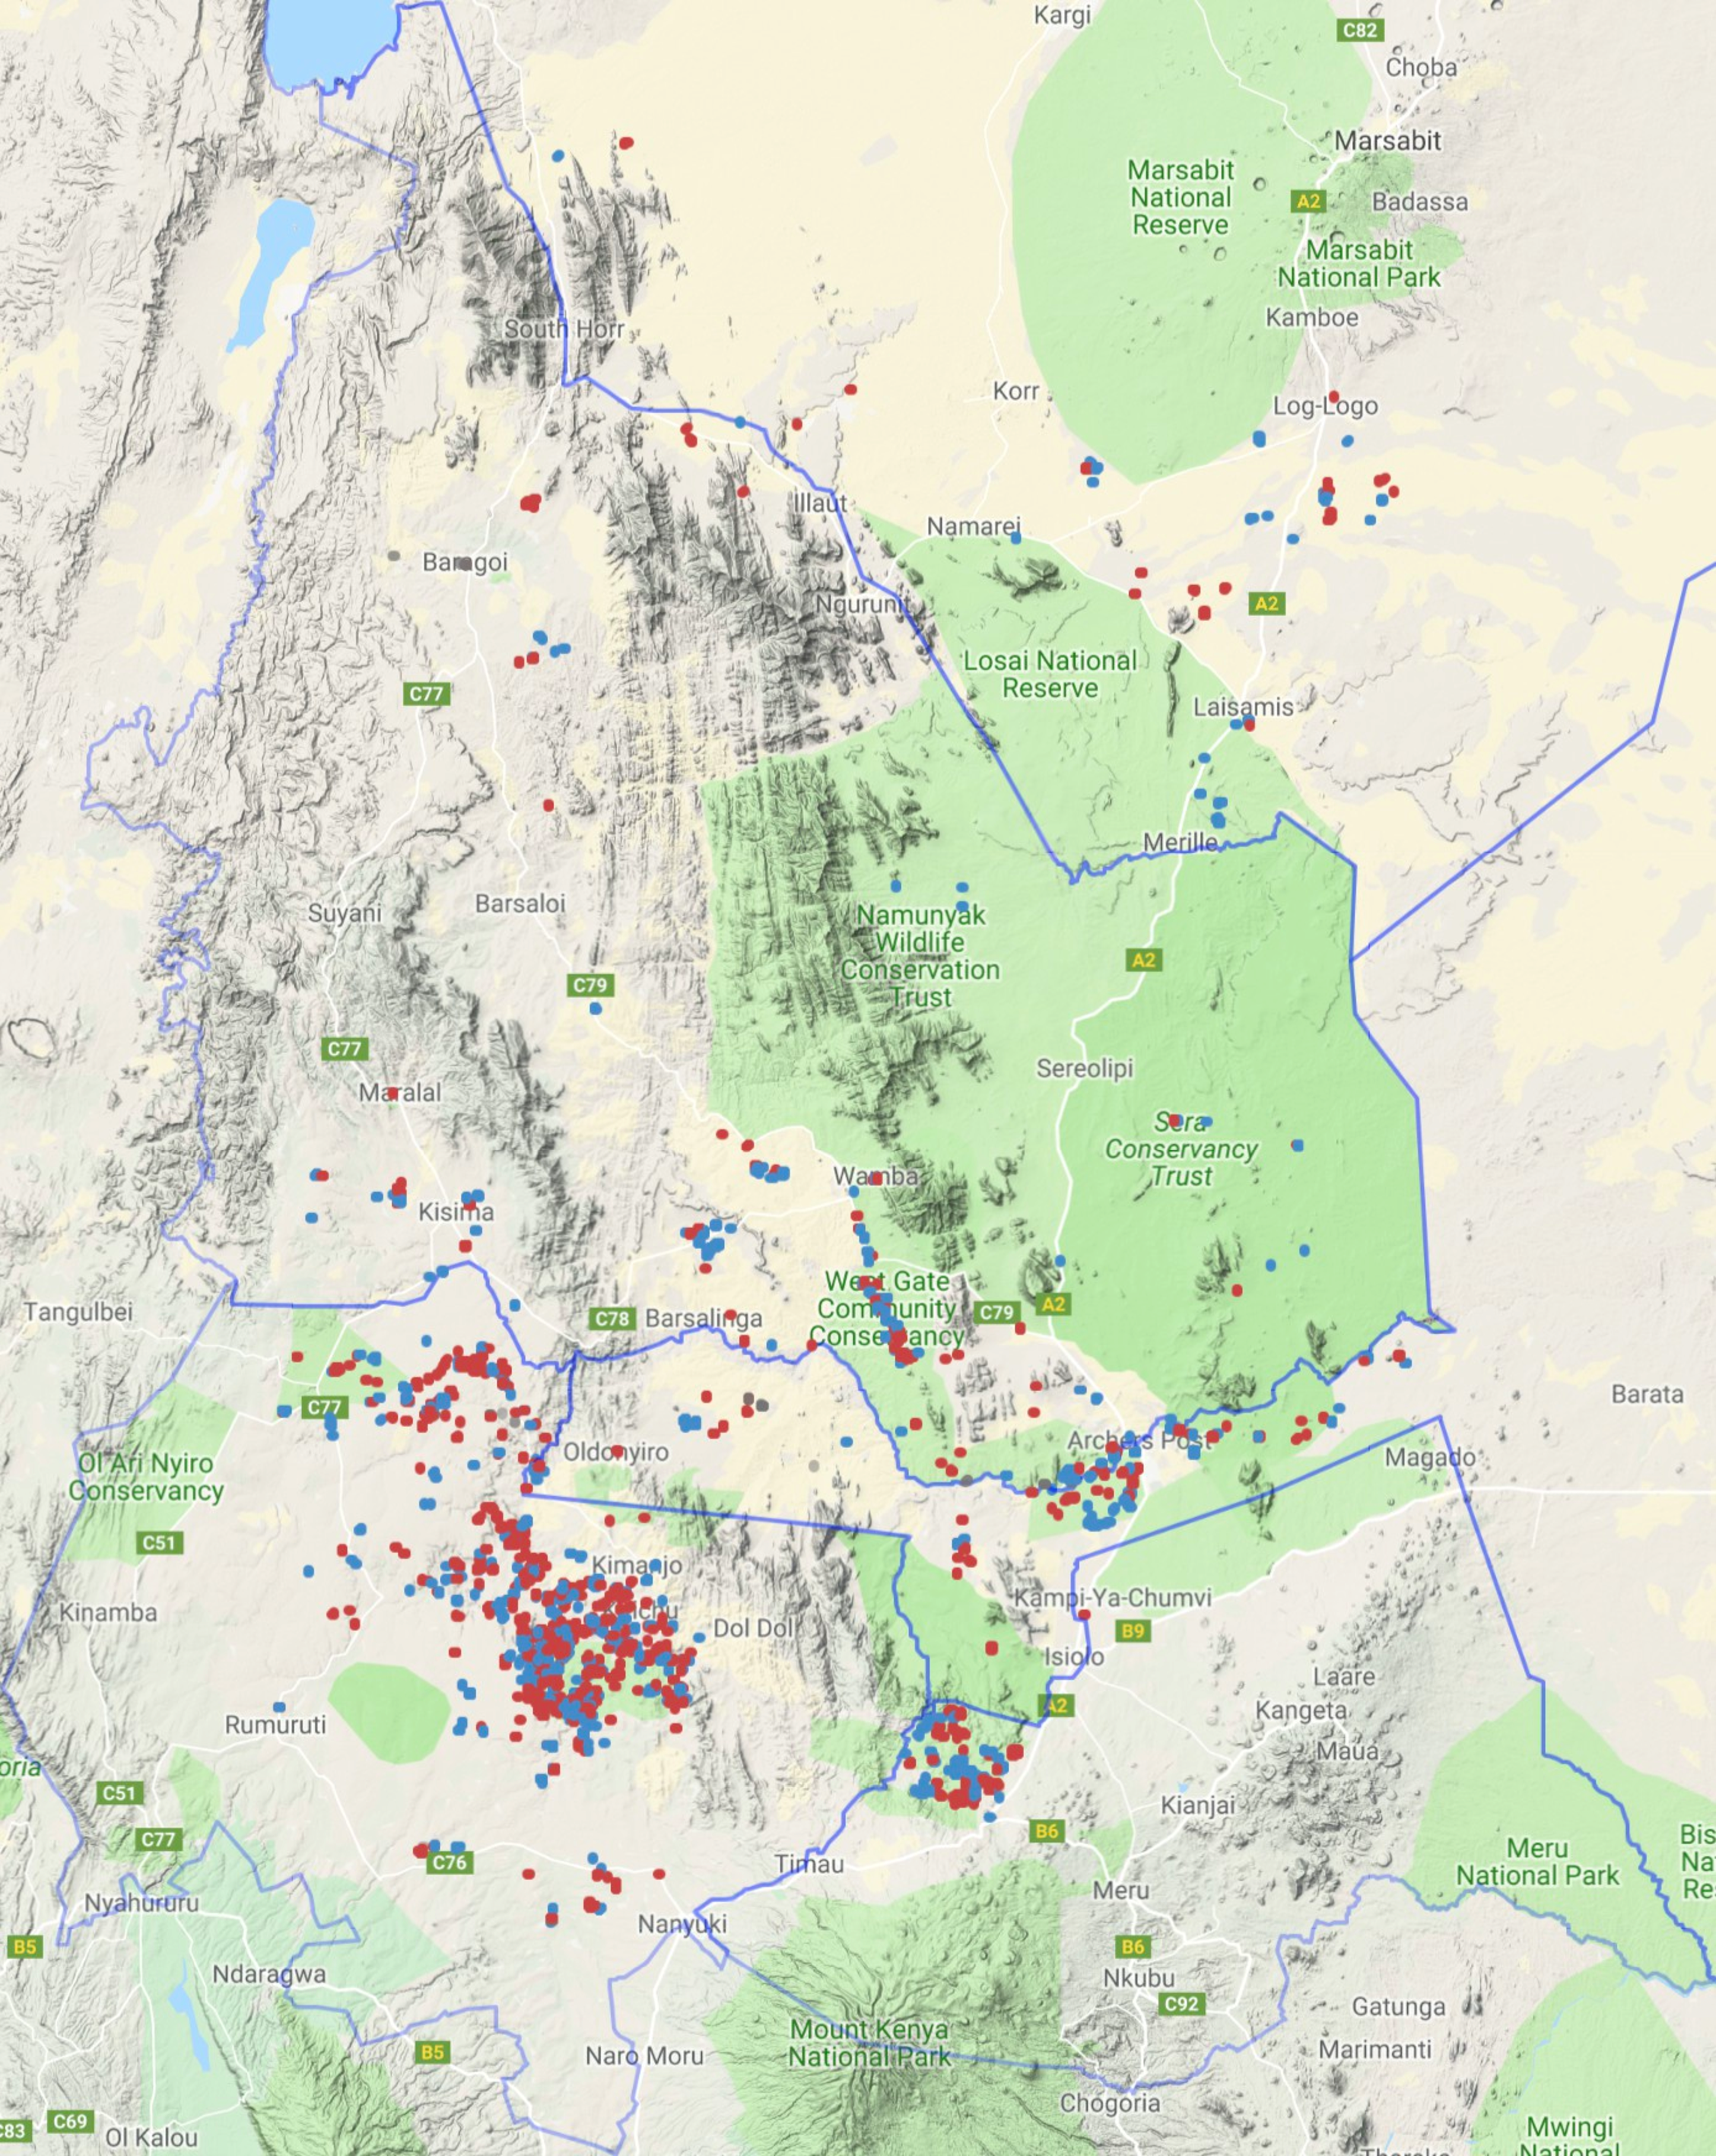
\includegraphics[width=0.83\linewidth]{resources/ggr2016.pdf}
    \end{center}
    \caption{The map of image GPS locations from the GGR-16 censusing rally.  Colored dots indicate sightings during the two days of each census; red were from day 1 only, blue were day 2 only, purple were resightings, and gray were unused.  The blue area lines indicate Kenyan county boundaries.  Rendered with Google Maps. Best viewed in color.  \copyright 2018 IJCAI. Reprinted, with permission, from: J. Parham, C. Stewart, T. Berger-Wolf, D. Rubenstein, and J. Holmberg, ``The Great Grevy’s Rally: A review on procedure,'' in \textit{AI Wildlife Conserv. Workshop}, Stockholm, Sweden, Jul. 2018, pp.1–3.}
    \label{fig:maps-ggr16}
\end{figure}

\begin{figure}[!t]
    \begin{center}
        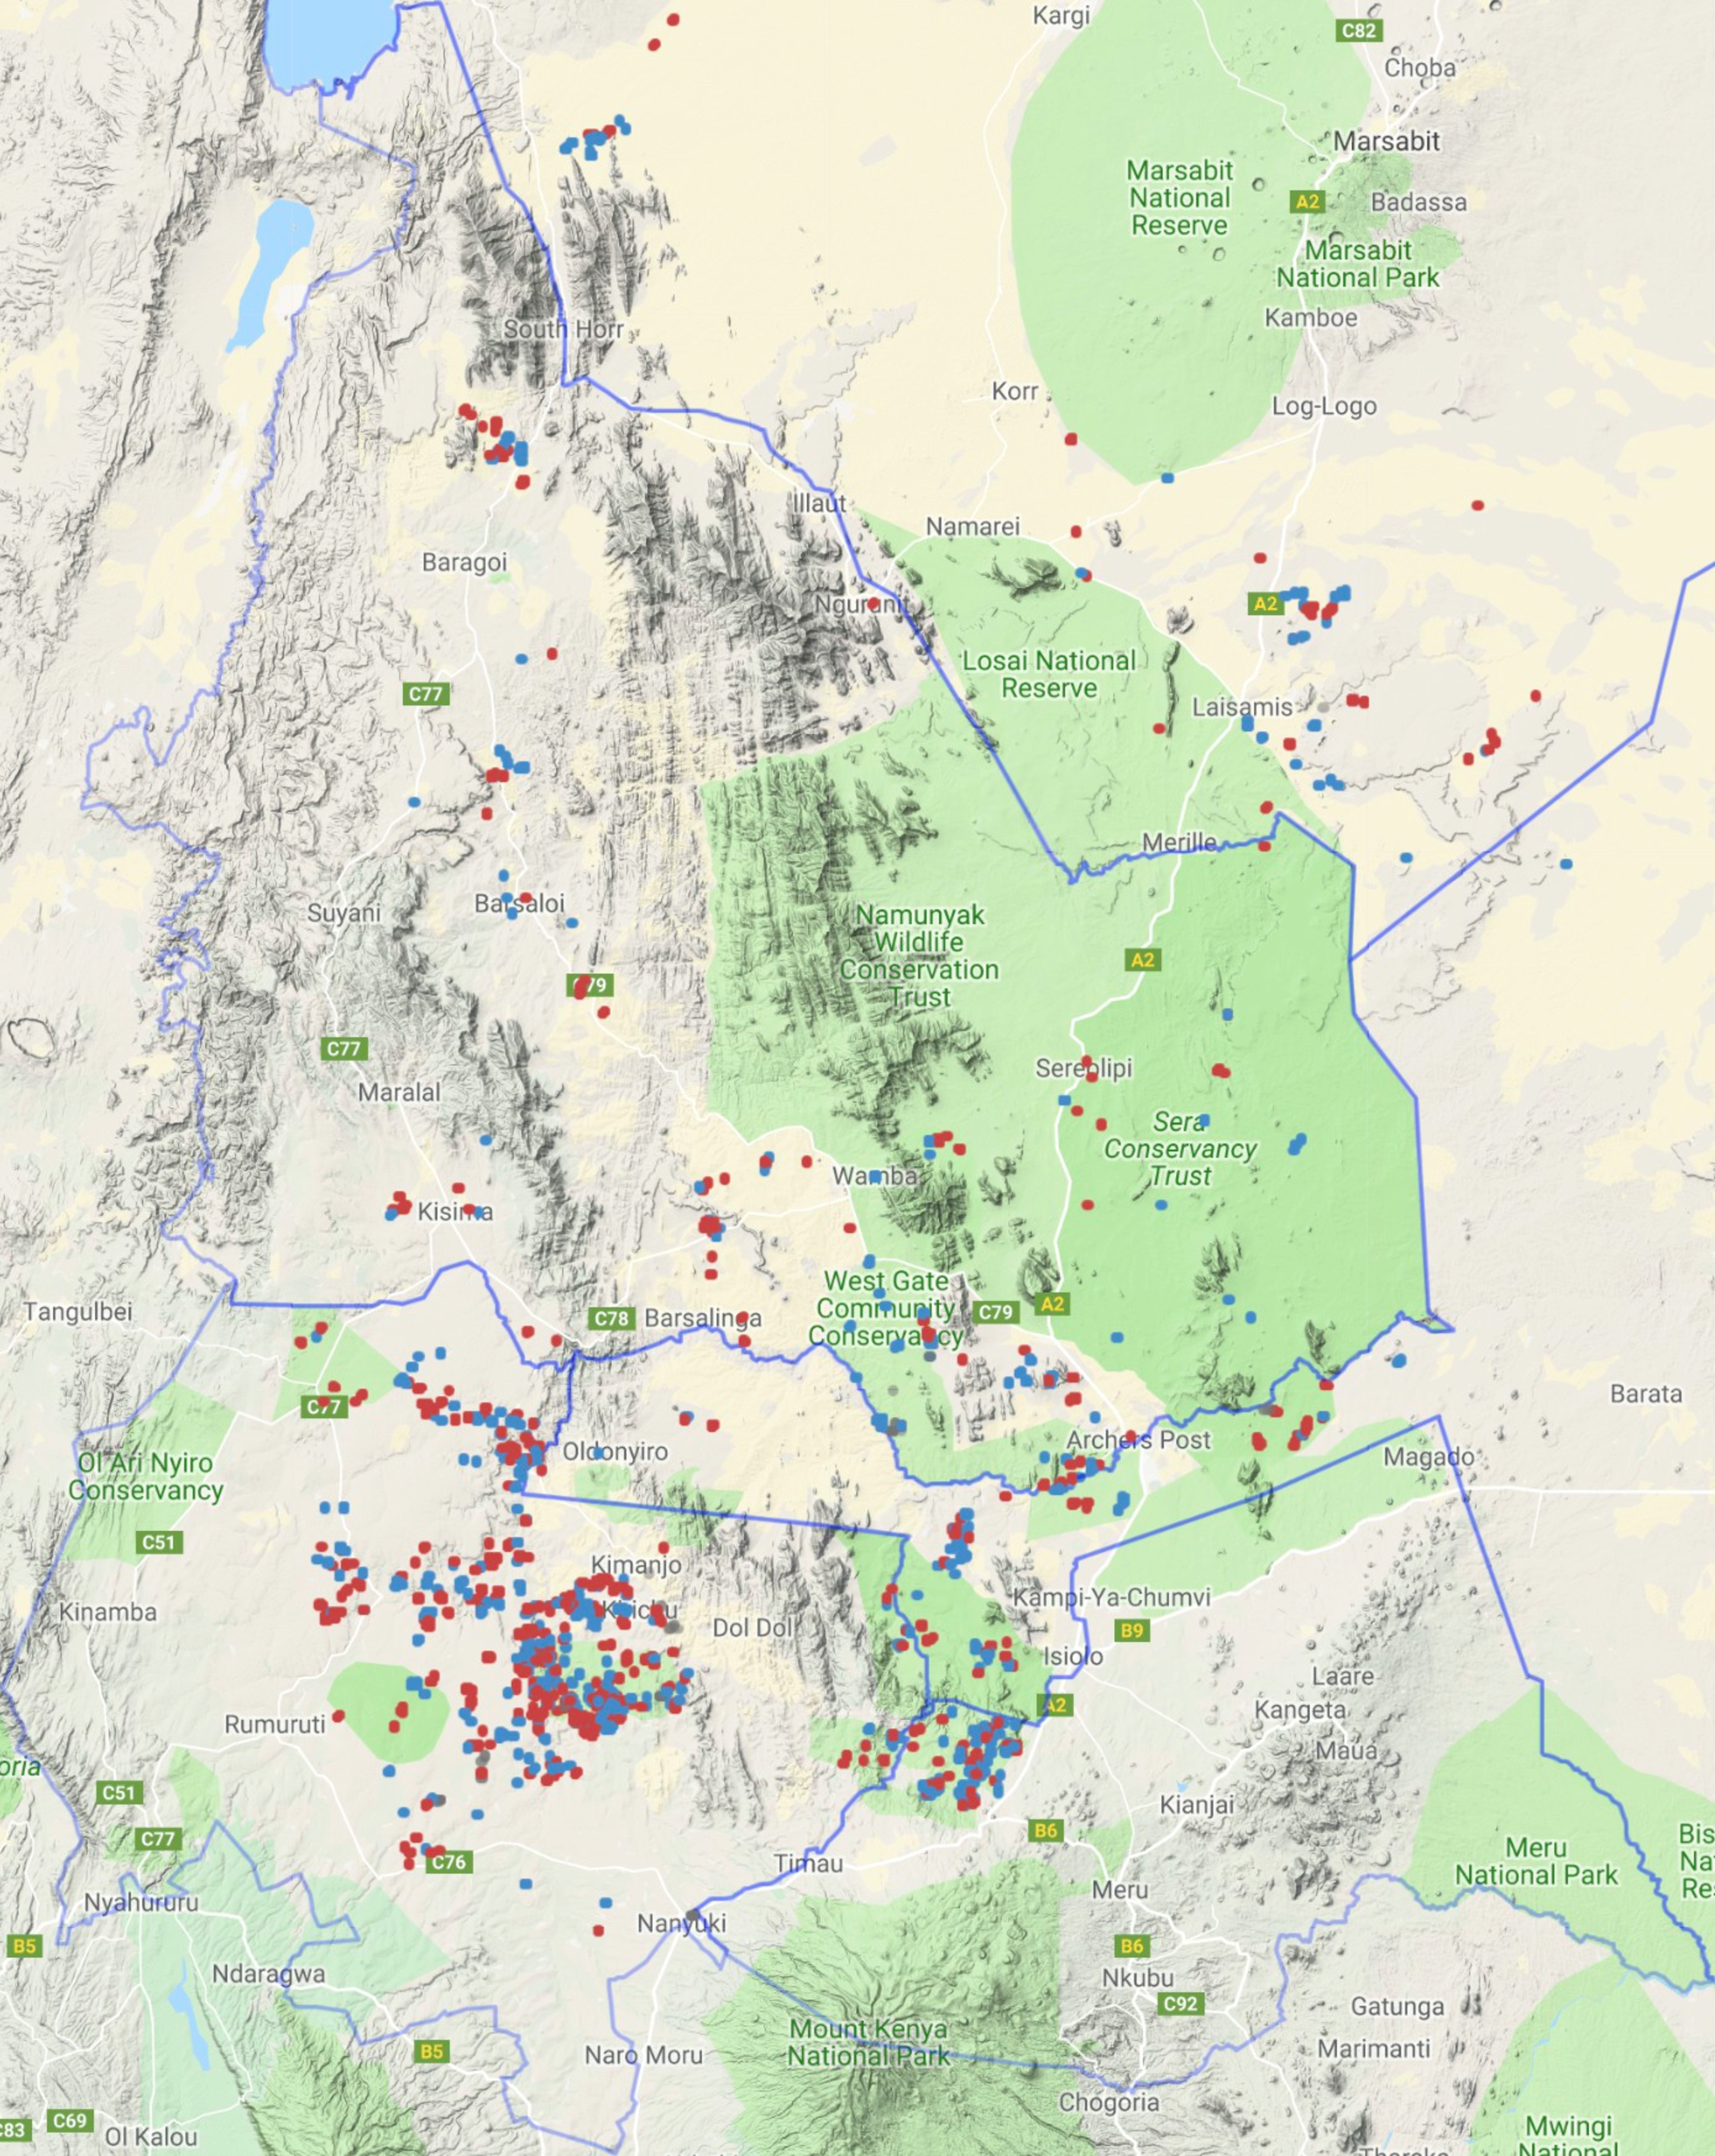
\includegraphics[width=0.83\linewidth]{resources/ggr2018.pdf}
    \end{center}
    \caption{The map of image GPS locations from the GGR-18 censusing rally.  Colored dots indicate sightings during the two days of each census; red were from day 1 only, blue were day 2 only, purple were resightings, and gray were unused.  The blue area lines indicate Kenyan county boundaries.  Rendered with Google Maps. Best viewed in color.  \copyright 2018 IJCAI. Reprinted, with permission, from: J. Parham, C. Stewart, T. Berger-Wolf, D. Rubenstein, and J. Holmberg, ``The Great Grevy’s Rally: A review on procedure,'' in \textit{AI Wildlife Conserv. Workshop}, Stockholm, Sweden, Jul. 2018, pp.1–3.}
    \label{fig:maps-ggr18}
\end{figure}

\subsubsection{Adherence to Training Instructions}

\begin{figure}[!t]
    \begin{center}
        \hspace*{-0.2in}
        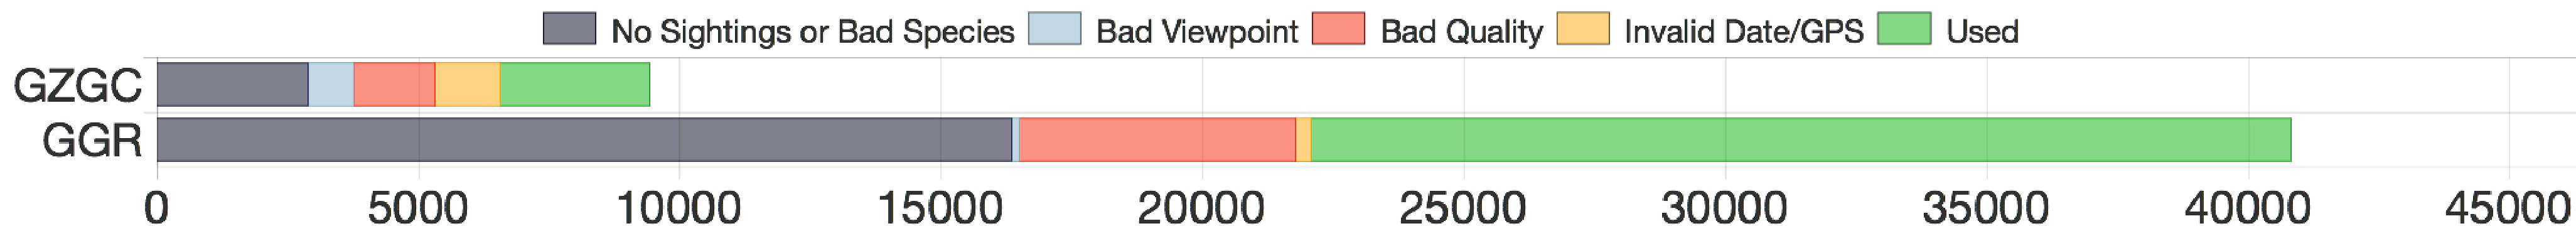
\includegraphics[width=1.0\linewidth]{resources/images-used-breakdown.pdf}
    \end{center}
    \caption{The numbers of collected photographs from the GZGC and GGR-16 and how they were used.  A large number (gray) were filtered out simply because they had no sightings or captured distracting species.  We further filtered the photographs taken of undesired viewpoints and had poor quality.  Lastly, we filtered photographs that were not taken during the two days of each rally (some volunteers brought their cameras with non-empty personal memory cards) or had corrupt/invalid GPS.  \copyright 2017 AAAI. Reprinted, with permission, from: J. Parham, J. Crall, C. Stewart, T. Berger-Wolf, and D. I. Rubenstein, ``Animal population censusing at scale with citizen science and photographic identification,'' in \textit{AAAI Spring Symp.}, Palo Alto, CA, USA, Jan. 2017, pp. 37–44.}
    \label{fig:breakdown-images-all}
\end{figure}

Now that the images have been collected from the volunteer photographers, we wish to analyze how well the resulting images conform to the provided training instructions.  Fir the GZGC and GGR-16, all annotations were created by hand, and viewpoints were added to determine how well the citizen scientists followed the data collection protocols.  As discussed earlier, citizen scientists were instructed first to take photographs from specific viewpoints on the animals -- left side during the GZGC and right sides for Gr\'evy's zebras (GGR-16) -- and then take additional photographs if they desired.  As such, the distribution of viewpoints is a strong indicator of adherence to the protocol. For example, Figure~\ref{fig:breakdown} (left) shows that around 50\% of the photographs in the GZGC and GGR-16 had an annotation from the desired viewpoint (green).  Furthermore, when the photographs of neighboring viewpoints (yellow) are taken into account, the percentage grows to 60\%.  The graph in Figure~\ref{fig:breakdown-images-all} reinforces the argument of good adherence, showing how the photographs were used during the analysis.  The most significant percentage of photographs filtered out did not include animals of the desired species.  The second highest percentage was from poor photograph quality.  Even so, the number of photographs used is still around 50\% for the GGR-16.

\subsubsection{Geographic Coverage \& Image Distributions}

Despite a skewed distribution, there was still strong area coverage across all three census rallies.  The locations of images taken during the GZGC can be seen in Figure~\ref{fig:maps-gzgc}, GGR-16 in Figure~\ref{fig:maps-ggr16}, and GGR-18 in Figure~\ref{fig:maps-ggr18}.  Note that the maps shown in the figures are at vastly different scales (refer to Figure~\ref{fig:maps-kenya}), and the coverage plots in the GZGC essentially show the roads through the Nairobi National Park.  The park was split into five zones~\cite{parham_photographic_2015} to help enforce coverage, which was very good in most cases.  For the GGR, the 25,000 $\textrm{km}^2$ survey area was broken into 45 counting blocks with variation in the animal density due to the presence of human settlements and the availability of habitat and resources to sustain Gr\'evy's zebras.  These 45 blocks (comprised mainly of protected conservation areas) were further organized into one of 5 Kenyan counties covering the survey area: Isiolo, Laikipia, Marsabit, Meru, and Samburu.  The blue lines on the GGR maps show county boundaries.  The spatial distributions of resightings are pretty uniform for both rallies, indicating that the respective counting block partitioning schemes accomplished their intended goals.  Furthermore, there were also five zones for the GGR events to ensure geographically isolated areas were properly sampled (see the top of Figure 1 in~\cite{parham_animal_2017}).

\begin{figure}[!t]
    \begin{center}
        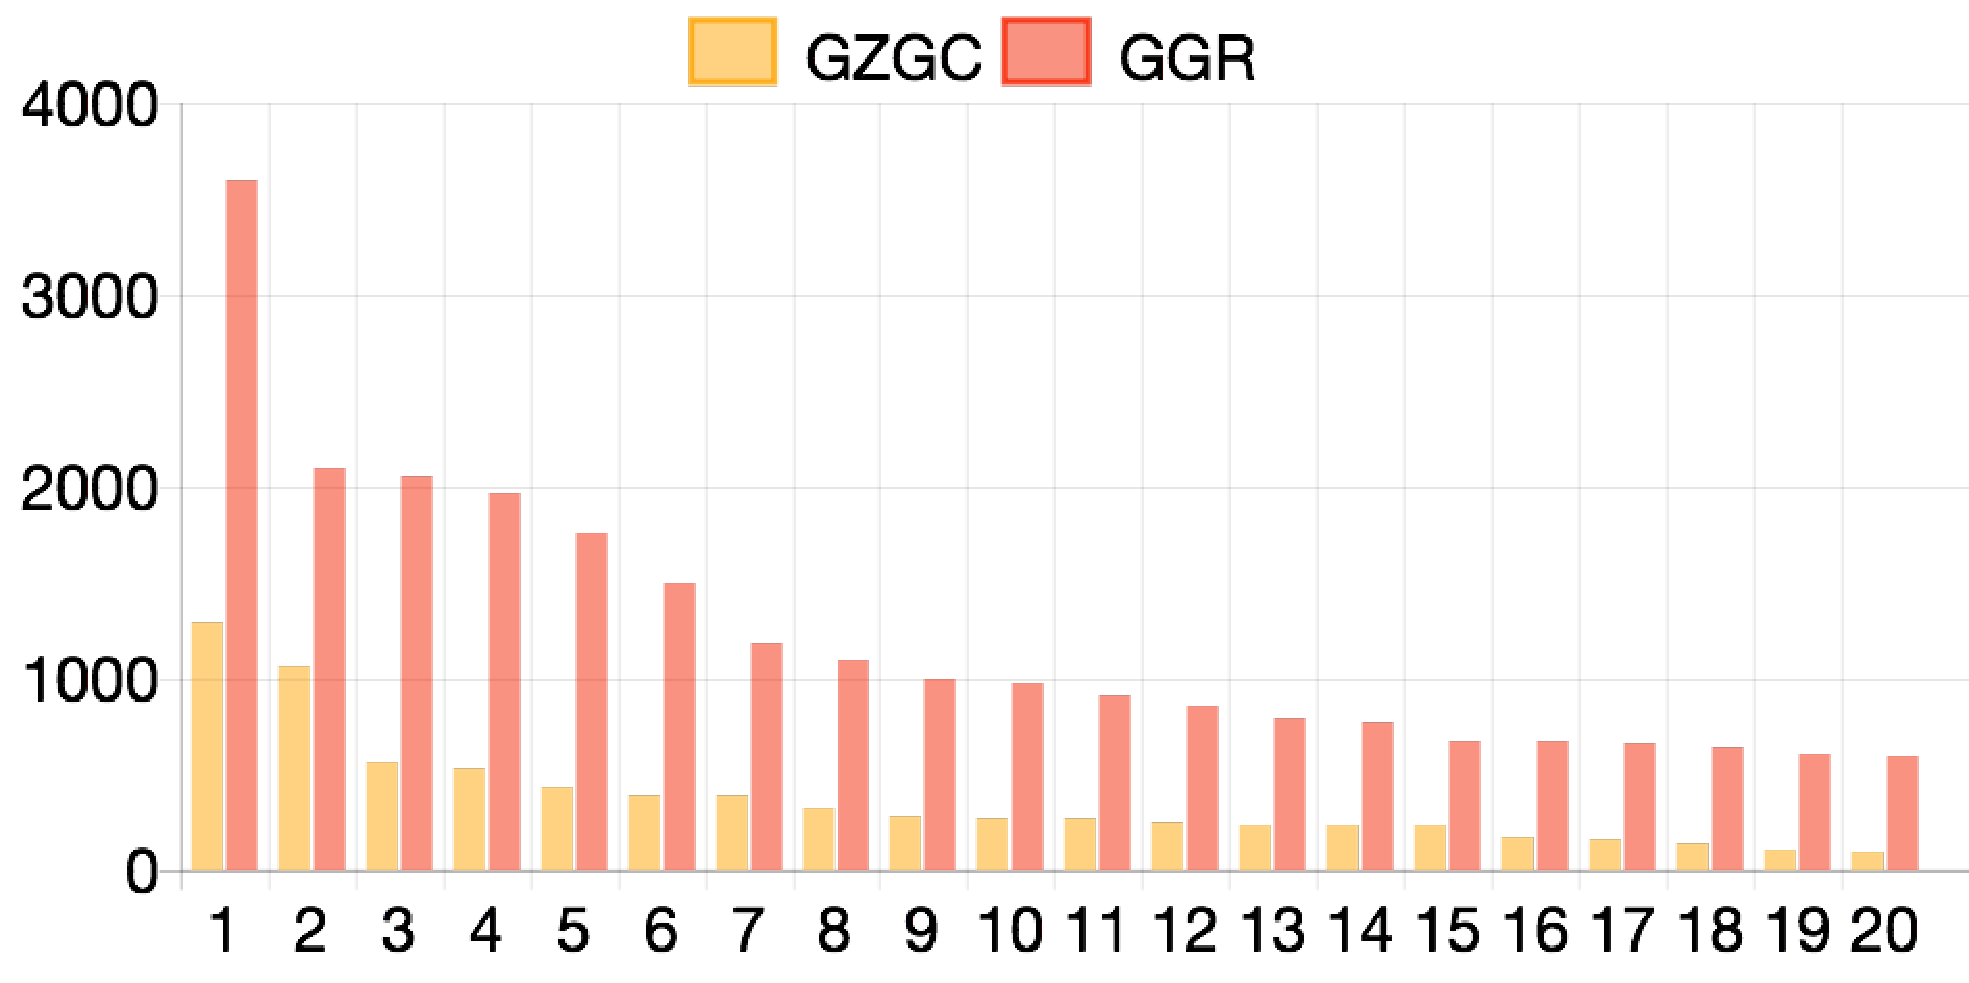
\includegraphics[width=0.95\linewidth]{resources/images-per-car.pdf}
    \end{center}
    \caption{The number of photographs taken by the top 20 cars during the GZGC and the GGR-16.  \copyright 2017 AAAI. Reprinted, with permission, from: J. Parham, J. Crall, C. Stewart, T. Berger-Wolf, and D. I. Rubenstein, ``Animal population censusing at scale with citizen science and photographic identification,'' in \textit{AAAI Spring Symp.}, Palo Alto, CA, USA, Jan. 2017, pp. 37–44.}
    \label{fig:cars}
\end{figure}

Figure~\ref{fig:cars} plots the distribution of photographs per camera.  We see that some photographers and cars are more prolific than others.  For example, the car that contributed the most images was nearly twice as productive as the second-most-productive car during the GGR-16 and produced nearly 3.5 times as many images as the most active car during the GZGC.  There are several possible reasons for the observed drop-off. In the GZGC, while some photographers were professional ecologists and conservationists, others were volunteers recruited on-site. Therefore, a significant difference in the commitment to take large quantities of photographs was expected.  For GGR-16, where volunteers were recruited in advance, the expertise was more uniform, but each car also had an assigned region, and the regions differed significantly in the expected density of animals.  A similar distribution was seen with the data collection for GGR-18, with some cars contributing a significant percentage of the photographs.  The key insight is that these high-volume photographers also sighted many individuals in the population and were assigned to areas with a known dense population.  As seen on the coverage maps, the areas with the most population also have the highest density of photographs.

\begin{figure}[!t]
    \begin{center}
        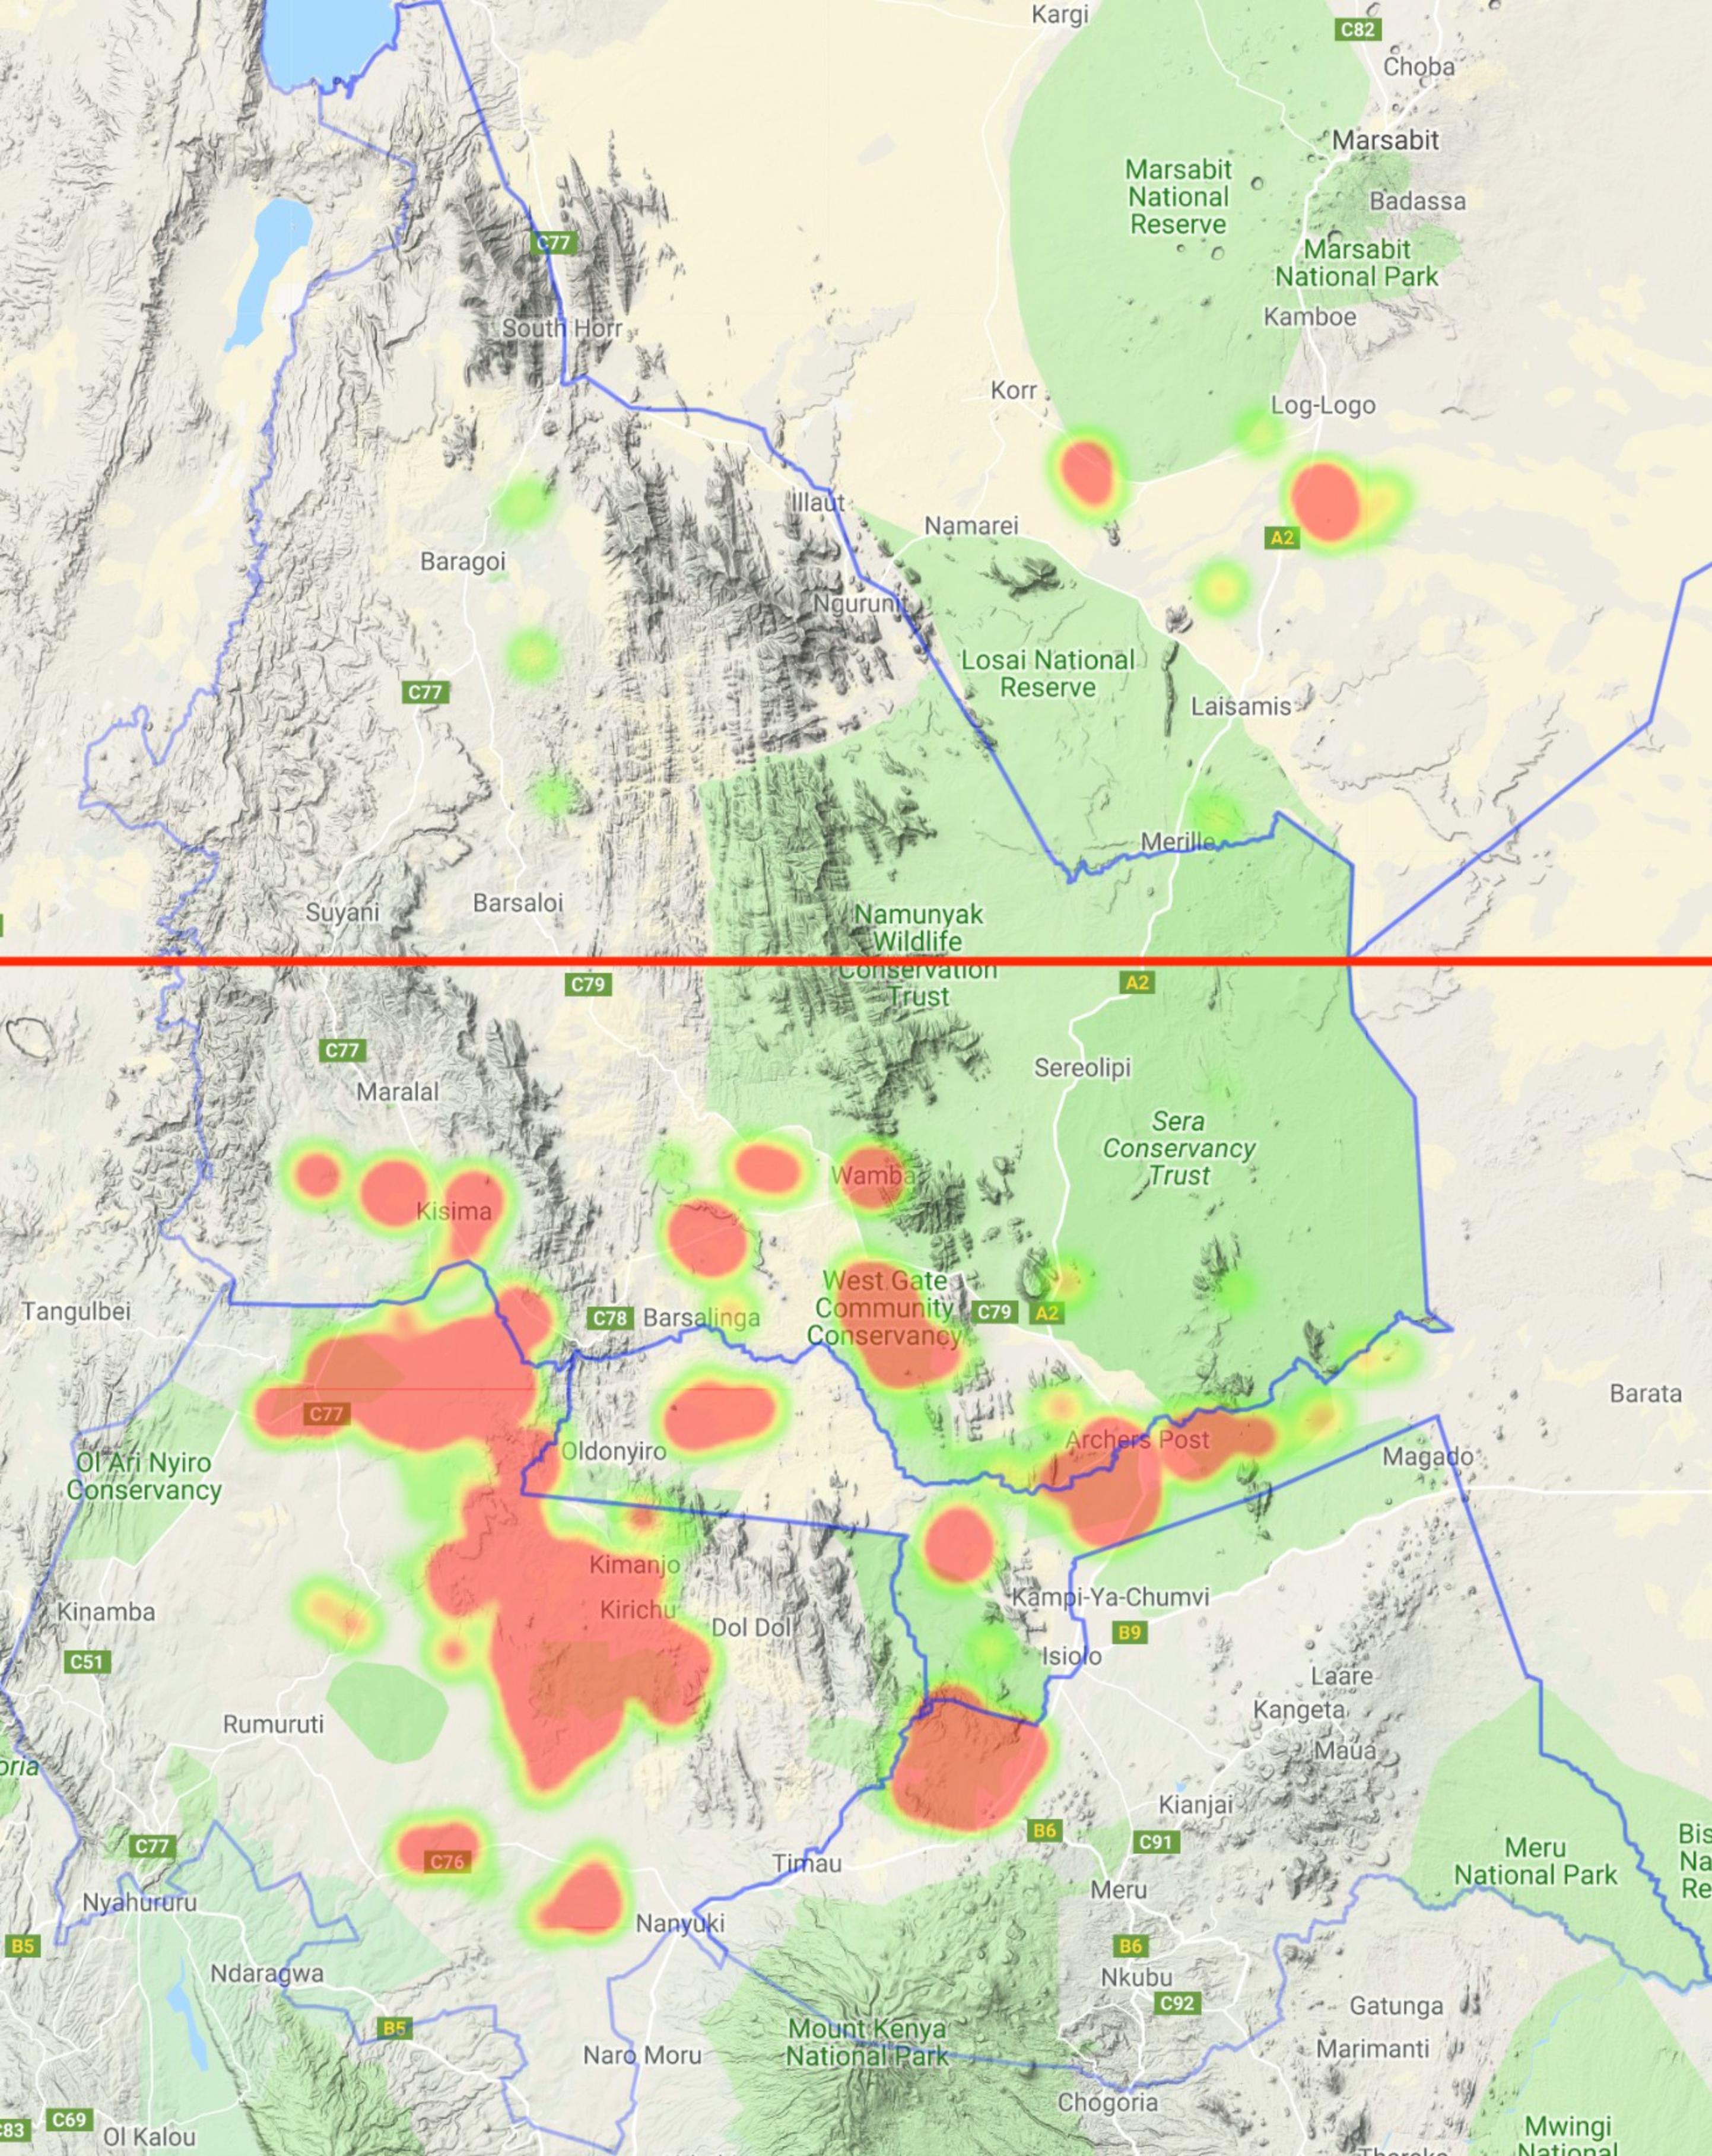
\includegraphics[width=0.45\linewidth]{resources/coverage-ggr2016-sightings-zebra.pdf}
        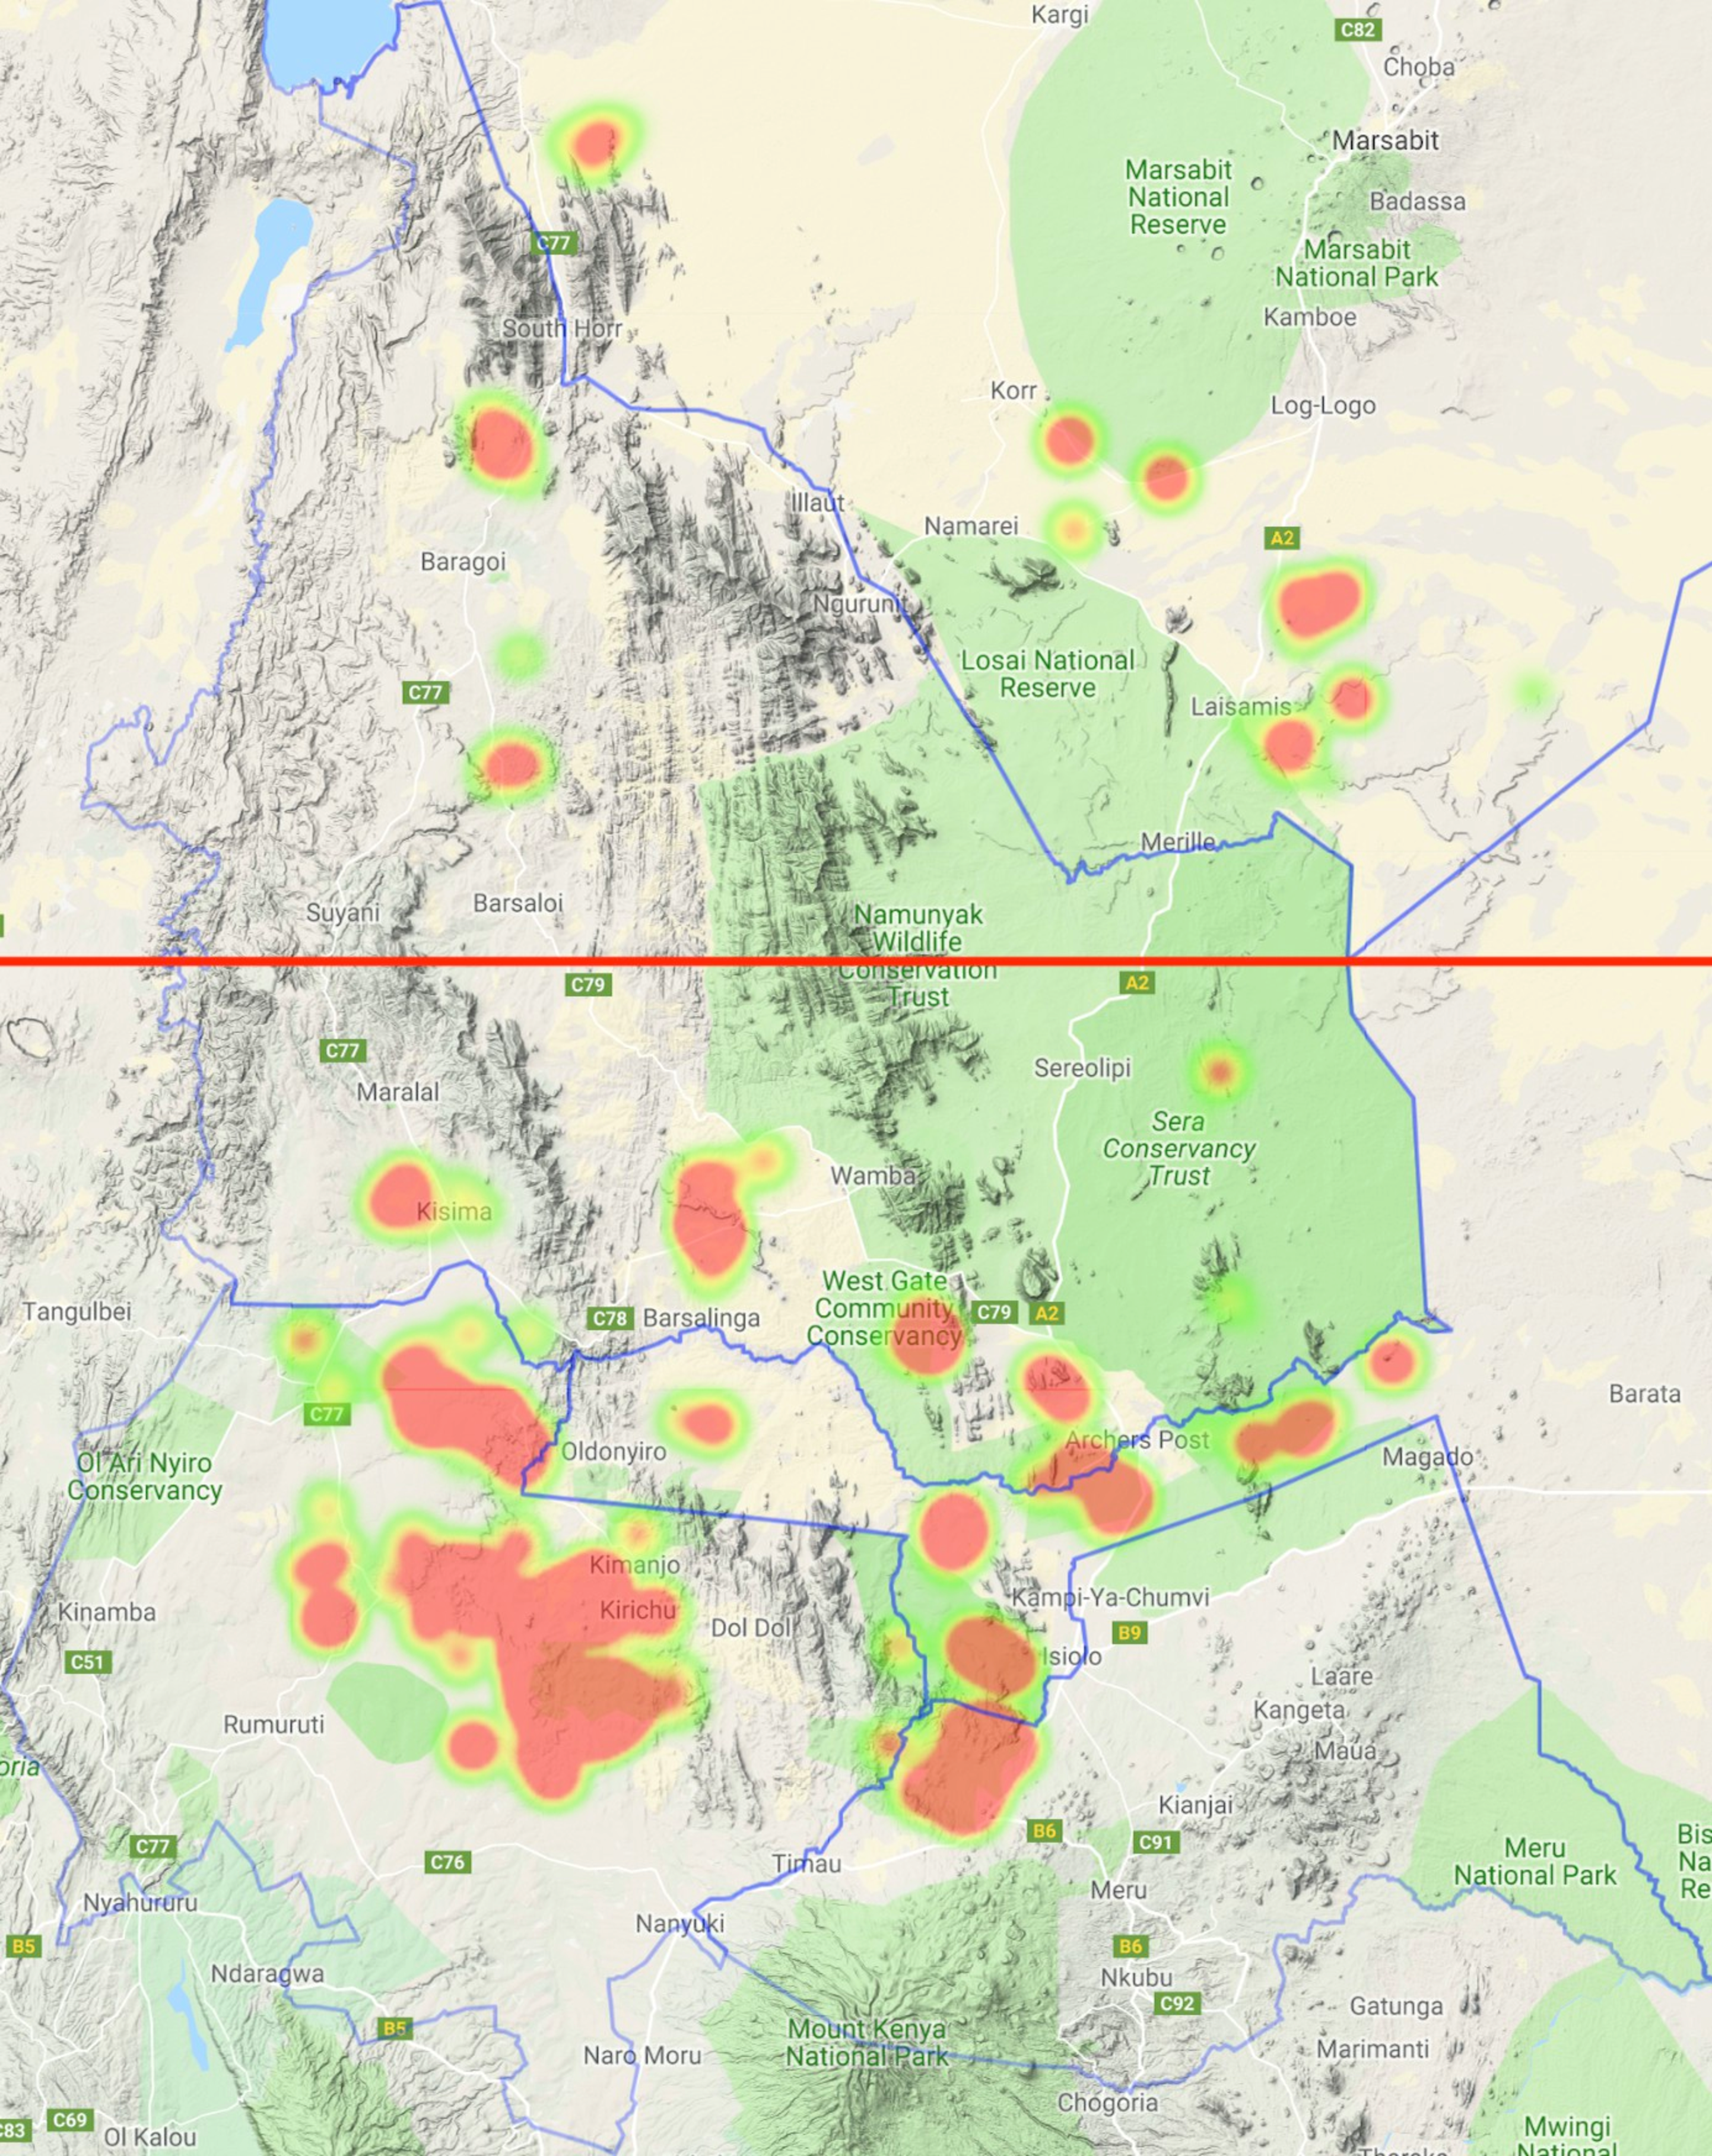
\includegraphics[width=0.45\linewidth]{resources/coverage-ggr2018-sightings-zebra.pdf}
    \end{center}
    \caption{A heatmap of identified animals captured during the GGR-16 and GGR-18 photographic censusing rallies.  The coverage in the northern blocks (above the red line) was improved during the GGR-18 (right) as compared to the GGR-16 (left).}
    \label{fig:maps-coverage}
\end{figure}

One of the known issues with the GGR-16 censusing rally was the poor coverage in the northern areas of the overall survey area.  During the GGR-18, additional participants were assigned explicitly to the northern areas, and the estimate essentially ``recovered'' approximately 400 animals that were missed during the first censusing rally.  Figure~\ref{fig:maps-coverage} shows a heat-map for the locations of identified zebras during the GGR-16 and GGR-18.  The red line indicates the delineation between the southern and northern blocks, showing that the GGR-18 census had a much more thorough coverage.  The county-by-county population statistics (which is shown in Table ~\ref{table:stats-county}) for the GGR-16 and GGR-18 also support this conclusion as the population estimates in the southern counties are stable over the two-year interval.  The northern region was simply not sampled thoroughly enough during the GGR-16, resulting in that area violating Assumptions 1 and 4 from Section~\ref{sec:assumptions}.

\subsection{Building the Animal ID Database}

The processing of the collected data\footnote{The GGR-16 and GGR-18 processing pre-dated the development of Census Annotations, Census Annotation Regions, and the LCA graph curation algorithm.} includes multiple stages and is designed to be a comprehensive pipeline that takes raw images as input and returns a set of named sightings with age and sex metadata. To provide a quick summary, we 1) curated a portion of the data for detection training with multiple reviewers per image, 2) trained the detection pipeline and applied it on all collected images, 3) used HotSpotter to rank all relevant annotations, 4) used the Graph ID algorithm to suggest manual review decisions to an asynchronous web interface or the VAMP automated decision algorithm and 5) asked ecologists to generate age and sex labels for all named individuals.

\subsubsection{Applying the Detection Pipeline}

\begin{figure}[!t]
    \begin{center}
        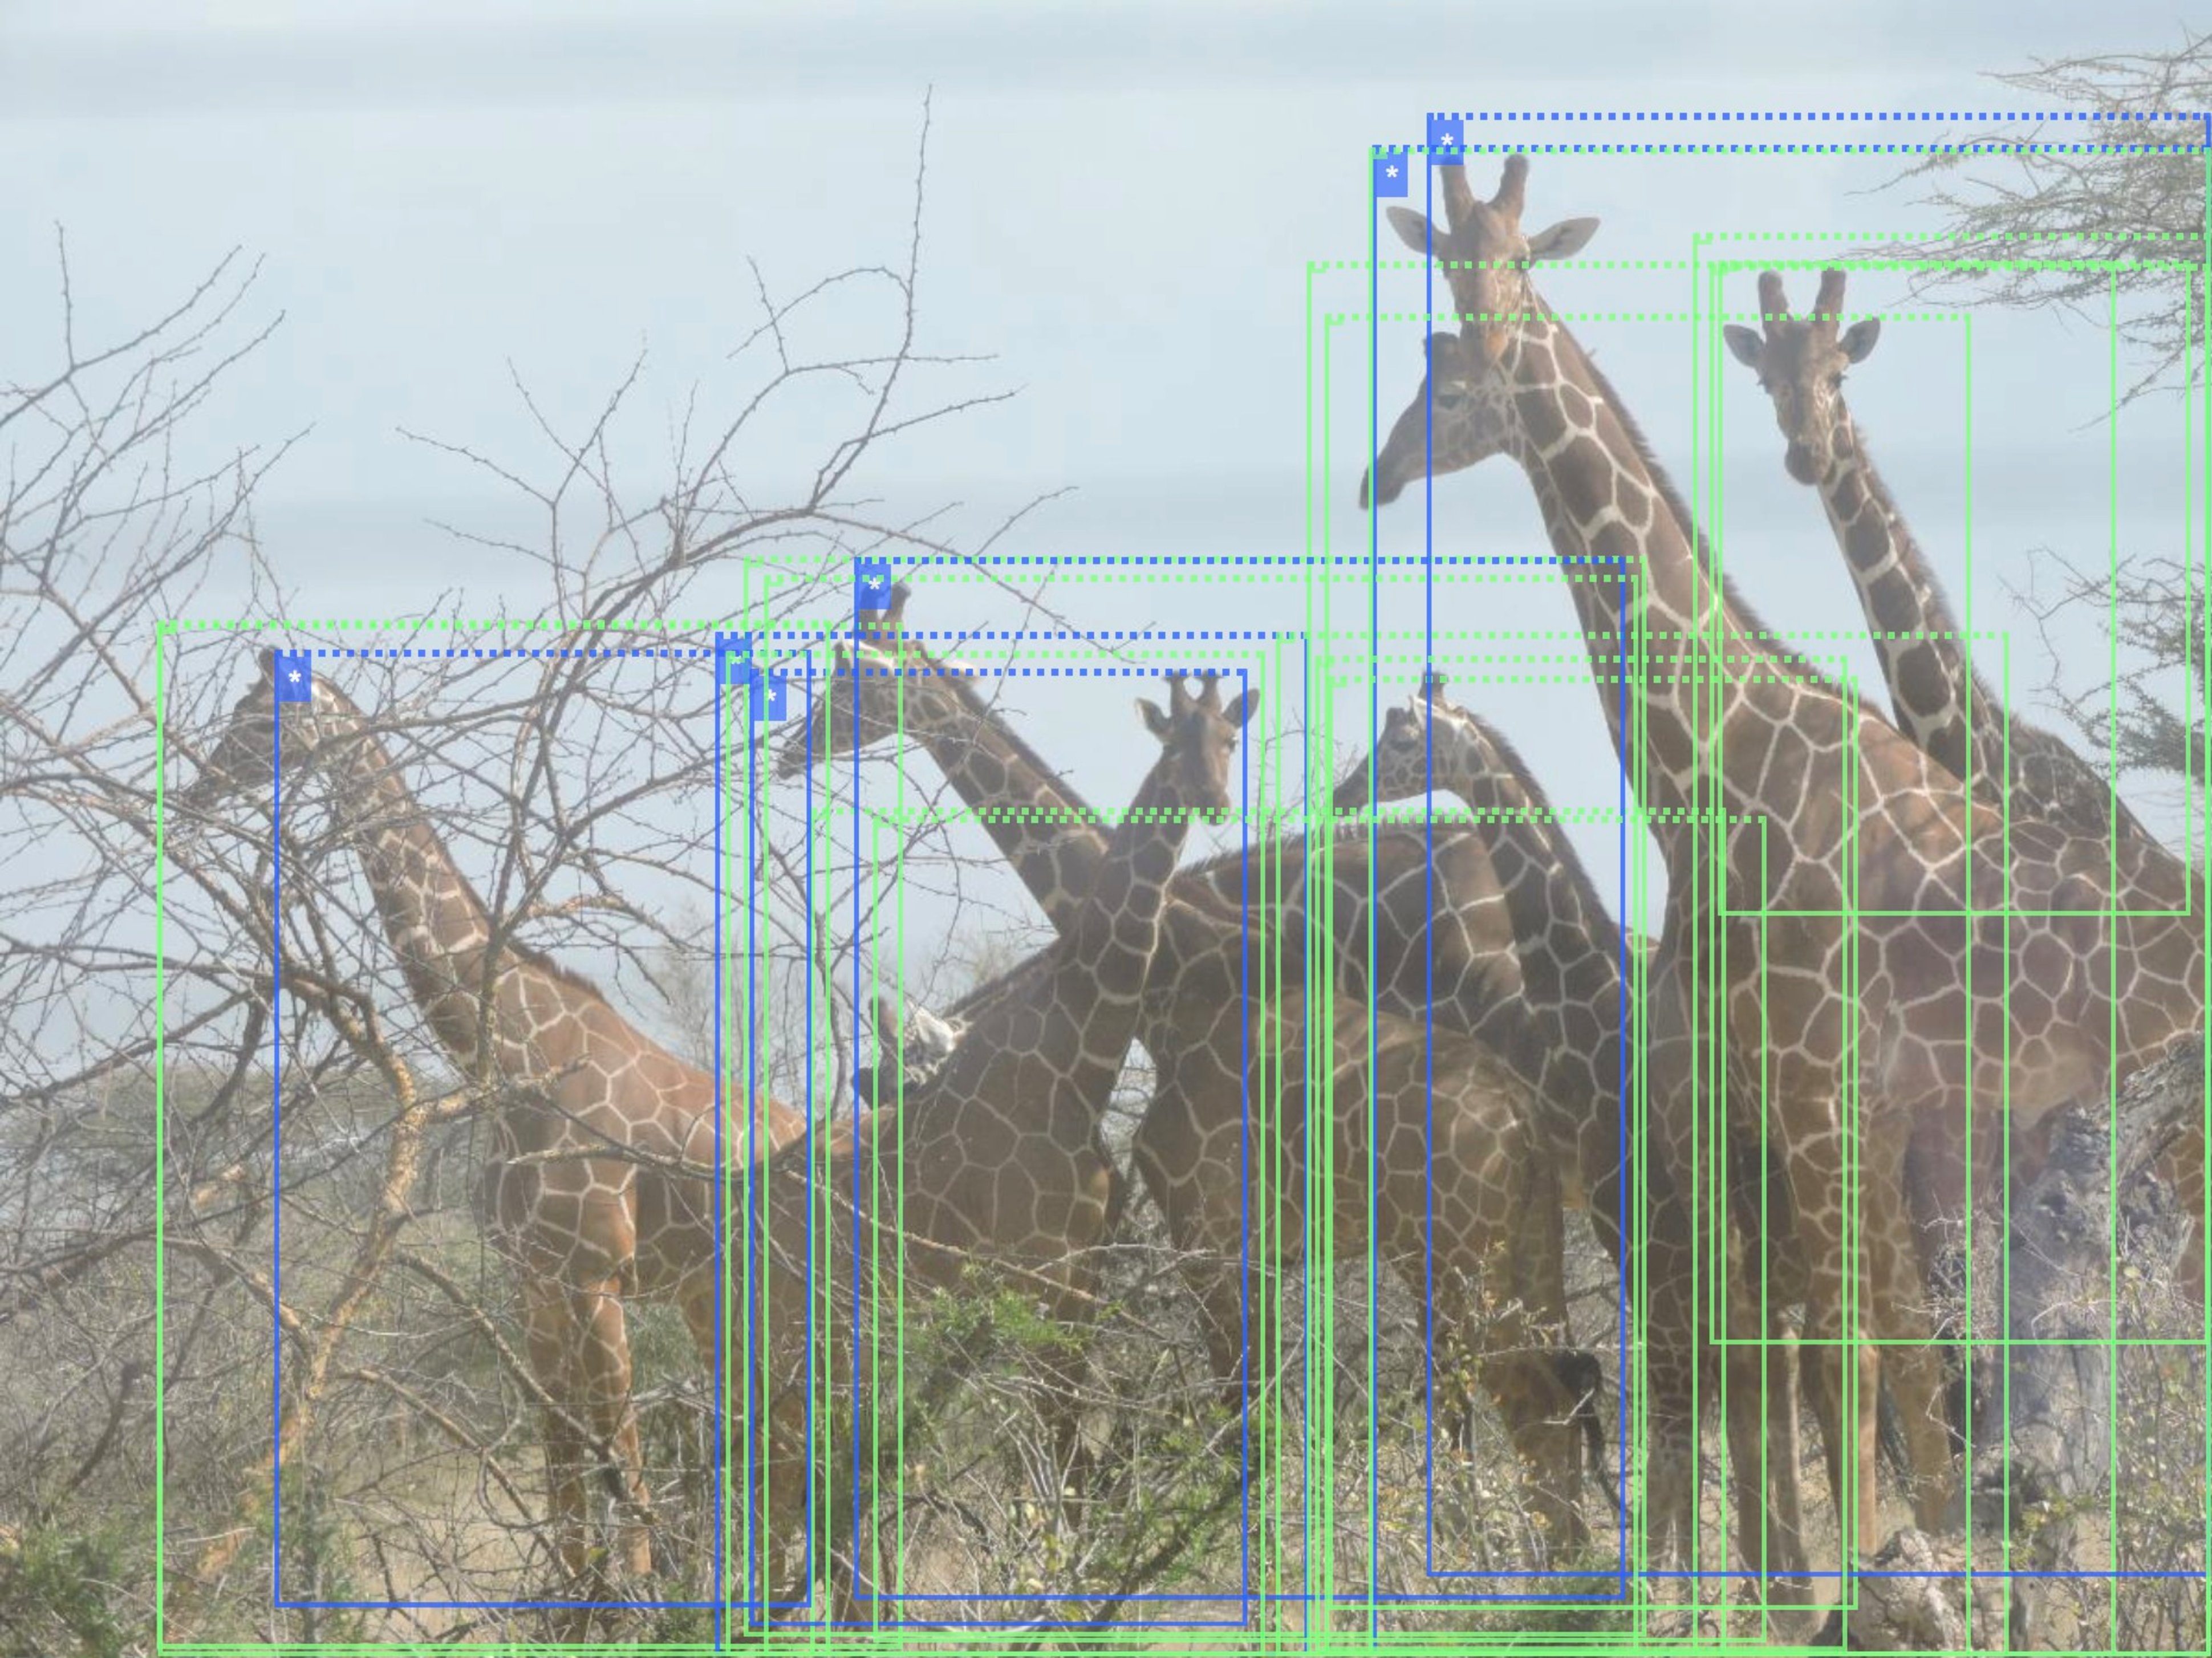
\includegraphics[width=0.45\linewidth]{resources/detections-example-unmerged.pdf}
        \vspace{2mm}
        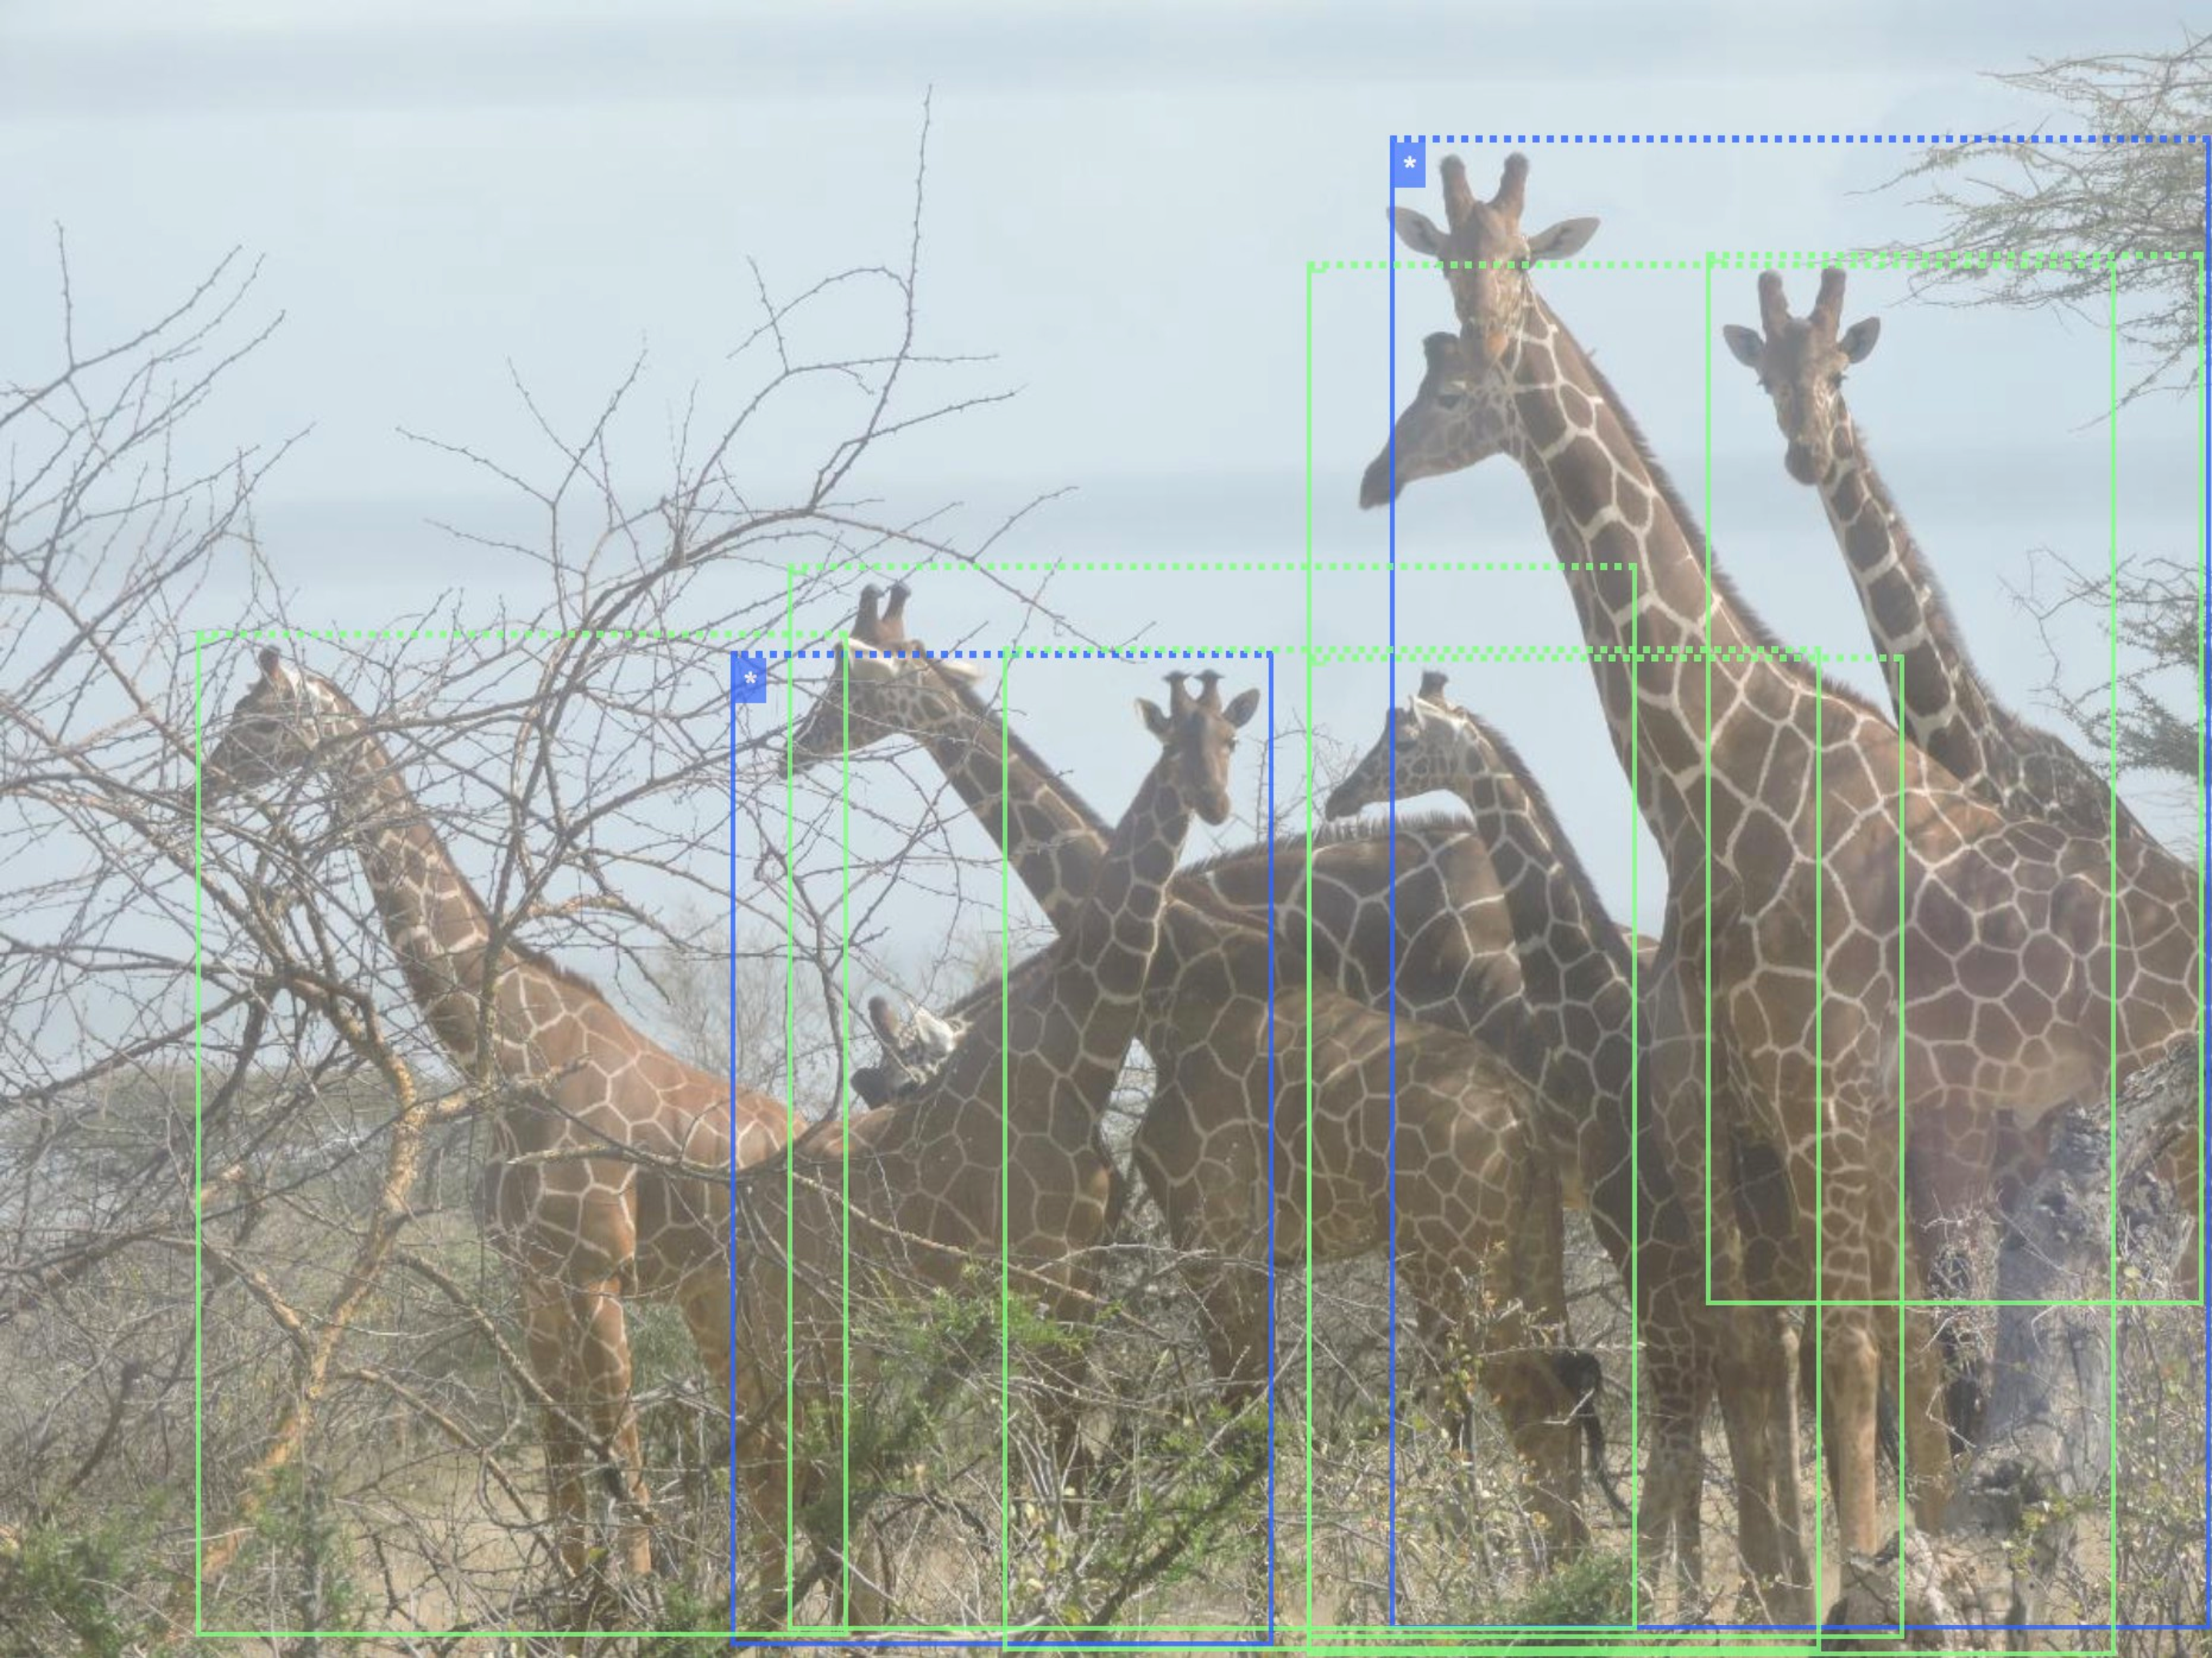
\includegraphics[width=0.45\linewidth]{resources/detections-example-merged.pdf}
    \end{center}
    \caption{An example image of giraffe from the GGR-18 photographic censusing rally, showing the input (left) and output (right) of the triple-marriage assignment problem.  Each image from the 10\% of annotated GGR-18 data is shown to three independent reviewers.  A triple-marriage algorithm is used to merge these into the final candidate bounding boxes (and AoI assignments) that are used for training the localizer.}
    \label{fig:marriage}
\end{figure}

\begin{figure}[!t]
    \begin{center}
        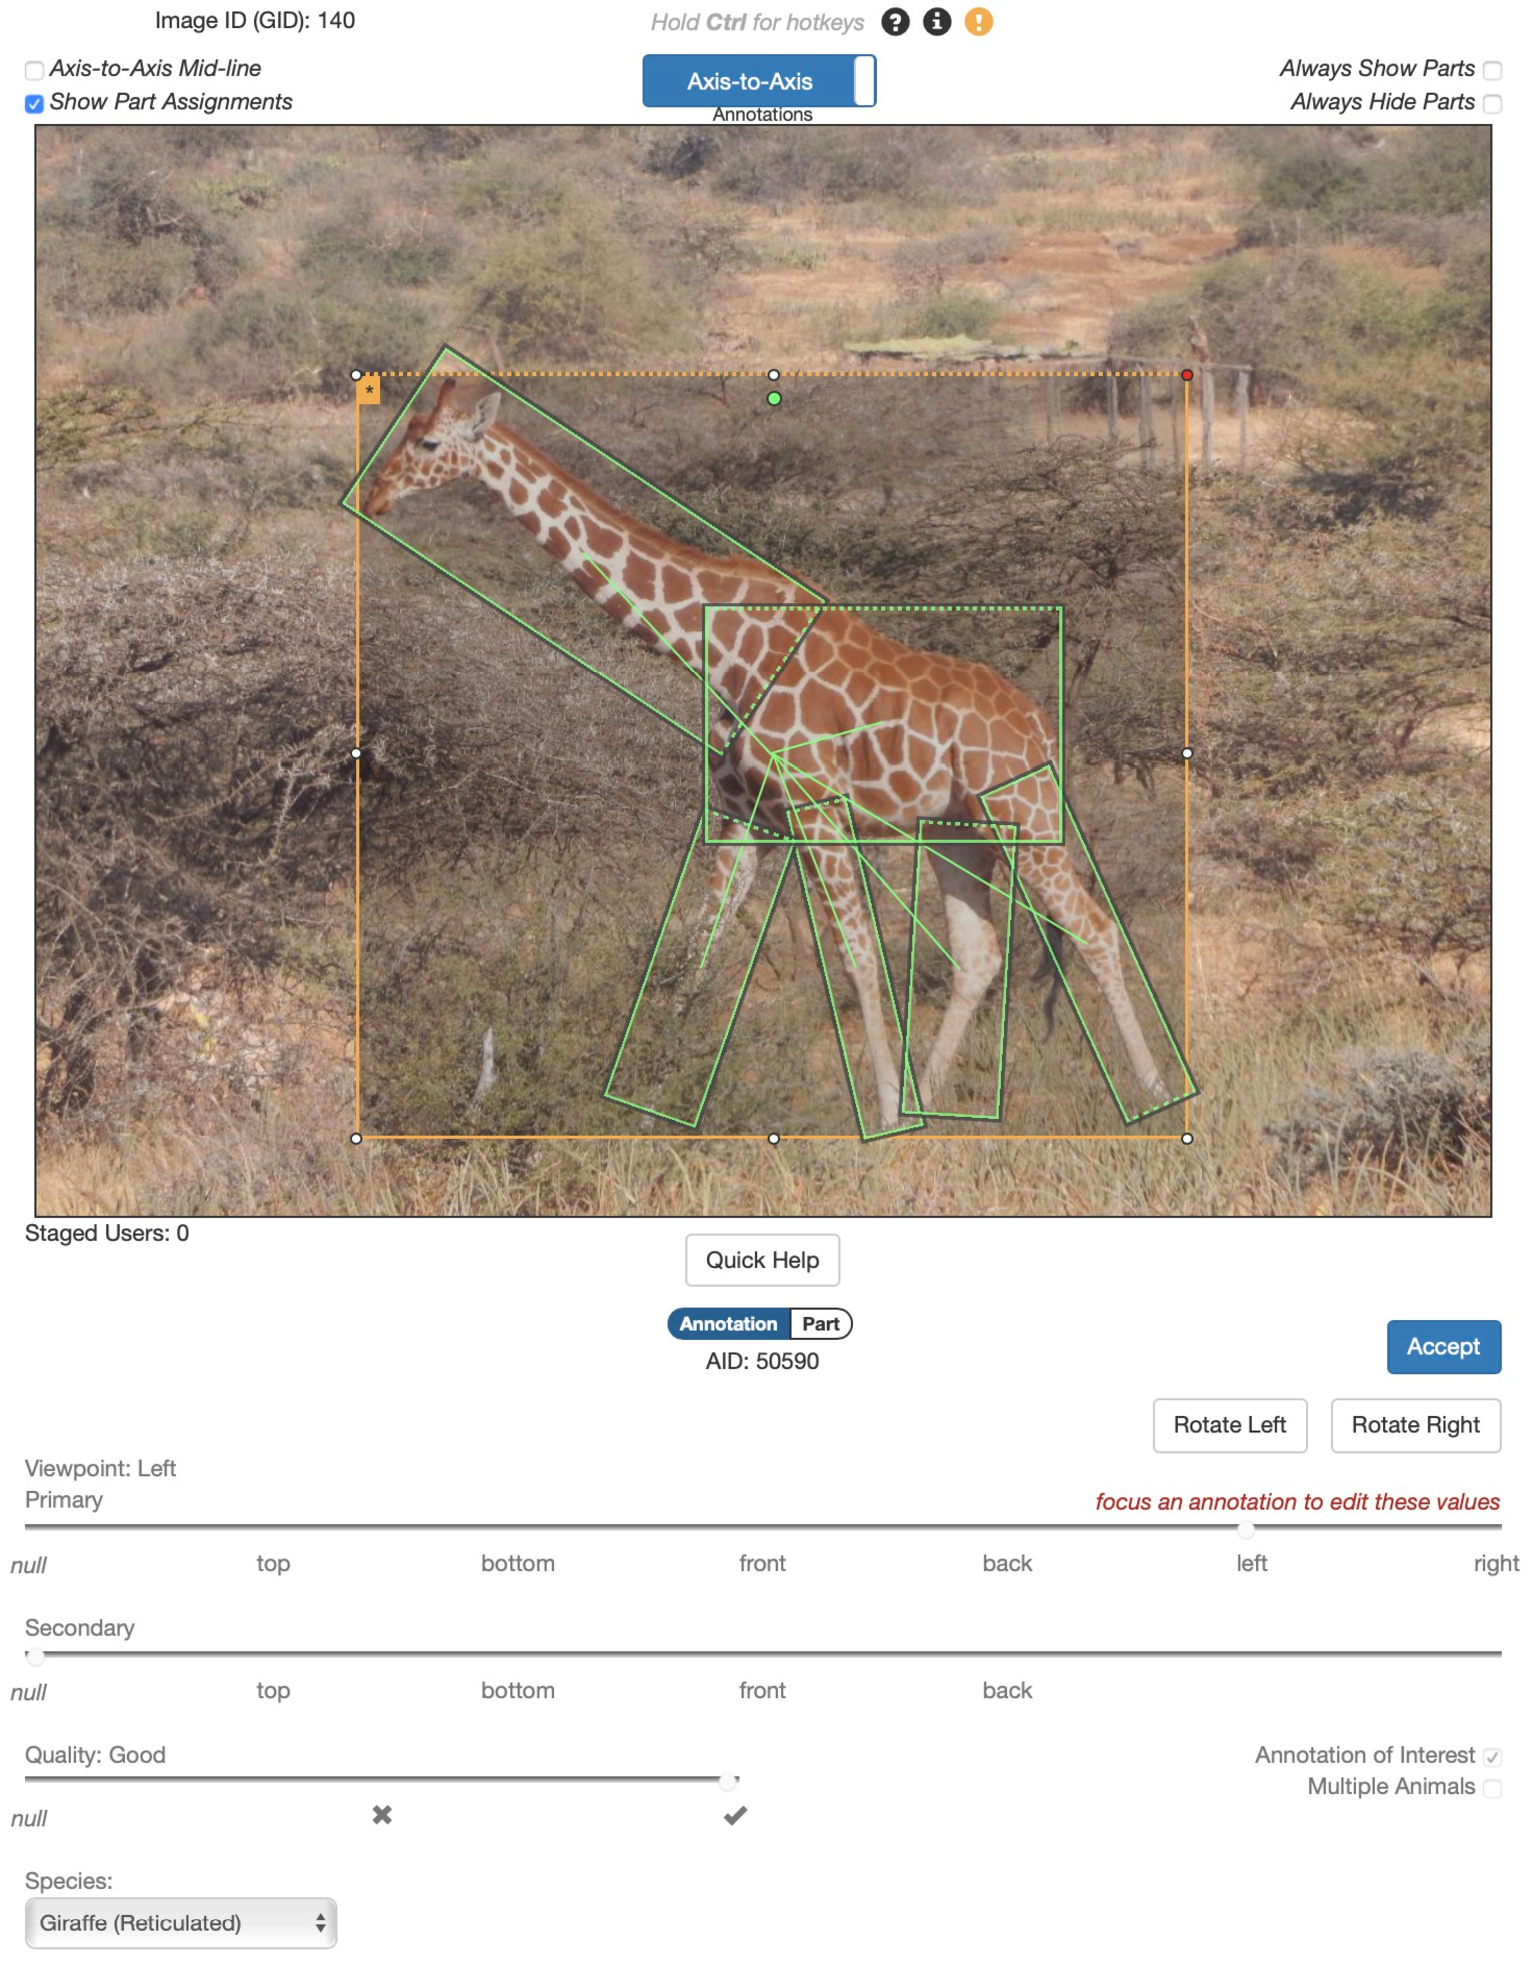
\includegraphics[width=0.85\linewidth]{resources/interface-detection.pdf}
    \end{center}
    \caption{An image of the updated web interface for bounding box annotation.  The updated interface was rewritten from the ground-up as used to annotate ground-truth data during the GZGC censusing rally.  The new interface is responsive, supports annotation parts and metadata, and is released as a public open-source tool.}
    \label{fig:interface-detection}
\end{figure}

New Gr\'evy's zebra and reticulated giraffe localization models were explicitly trained for the GGR-18, ignoring pre-existing models from the GGR-16 and GZGC.  These models were re-trained due to training process improvements (i.e., an updated Python implementation) and used annotations generated by a more robust bounding box collection methodology.  A total of 5,000 images were annotated for the GGR-18, with at least three independent reviewers for each image.  A pool of 14 reviewers was asked to annotate bounding boxes for 10\% of the dataset during the GGR-18.  The triple-reviewer procedure was not used with the GZGC or GGR-16 events for two reasons: 1) in the interest of time, the reviewers' workload was limited to one review per image (and done by hand for all images), and 2) the analysis of the GGR-18 data included the AoI component, which required more reliable and robust ground-truth annotations.  Since each image was annotated slightly differently by three individuals (and since AoI decisions are somewhat subjective), these bounding box candidates needed to be merged (or ``married'') into a set of finalized bounding box candidates.  A greedy three-person marriage algorithm compared the bounding boxes across the three reviewers, prioritizing the merging of boxes with the highest joint Intersection Over Union (IoU) percentages and starting with groups of three highly overlapping boxes (one from each reviewer).  This process continued until a threshold was met (IoU 25\%).  After all three-box marriages were assigned, a second round of two-box marriages was performed.  An example of a marriage solution can be seen in Figure~\ref{fig:marriage}.  Furthermore, AoI flags were determined independently for each annotation before the marriage assignments.  These flags are vital to properly tune the localization models to de-prioritize background animals.  Figure~\ref{fig:interface-detection} displays the web interface that the reviewers used to annotate all ground-truth detection data.  The interface was further updated since its use in the GZGC to add support for part bounding boxes.  The bounding boxes and their AoI assignments (seen in blue) for a given image are displayed together (left), and the final bounding boxes and AoI assignments are also shown (right).  The final AoI flag was determined by a majority vote, with married pairs of two being marked as an AoI if at least one reviewer considered their bounding box an AoI.

\begin{figure}[!t]
    \begin{center}
        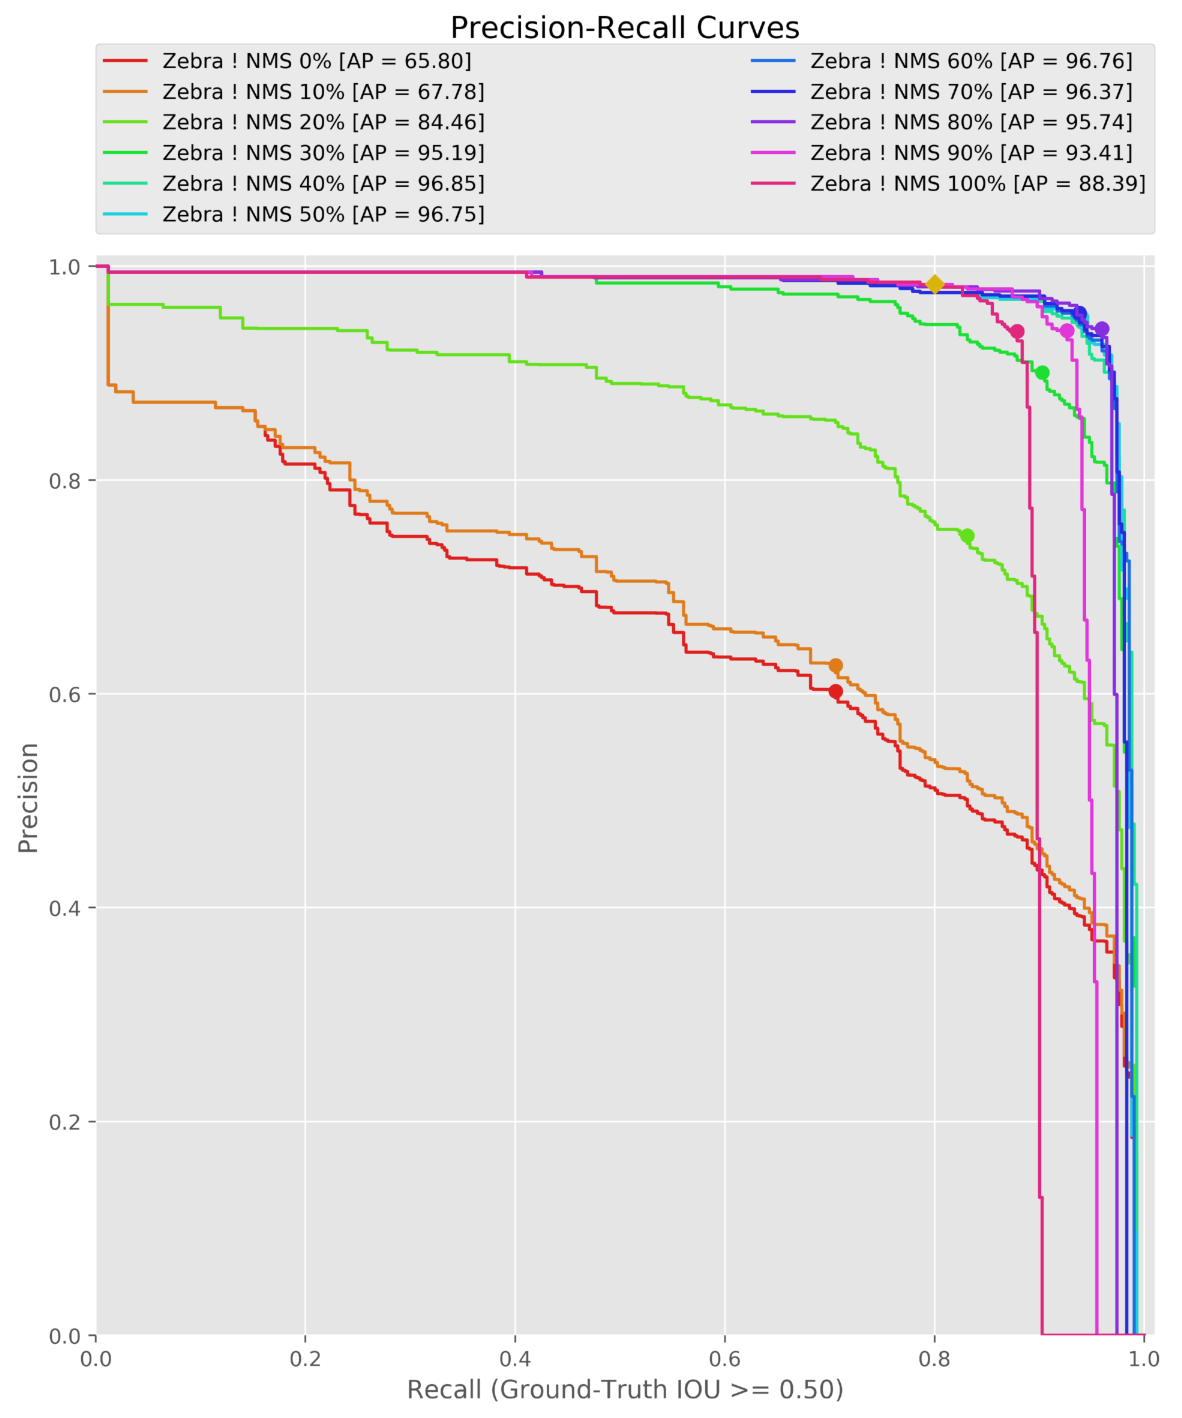
\includegraphics[width=0.45\linewidth]{resources/ggr2-!zebra-lightnet-localizer-precision-recall-50.pdf}
        \vspace{2mm}
        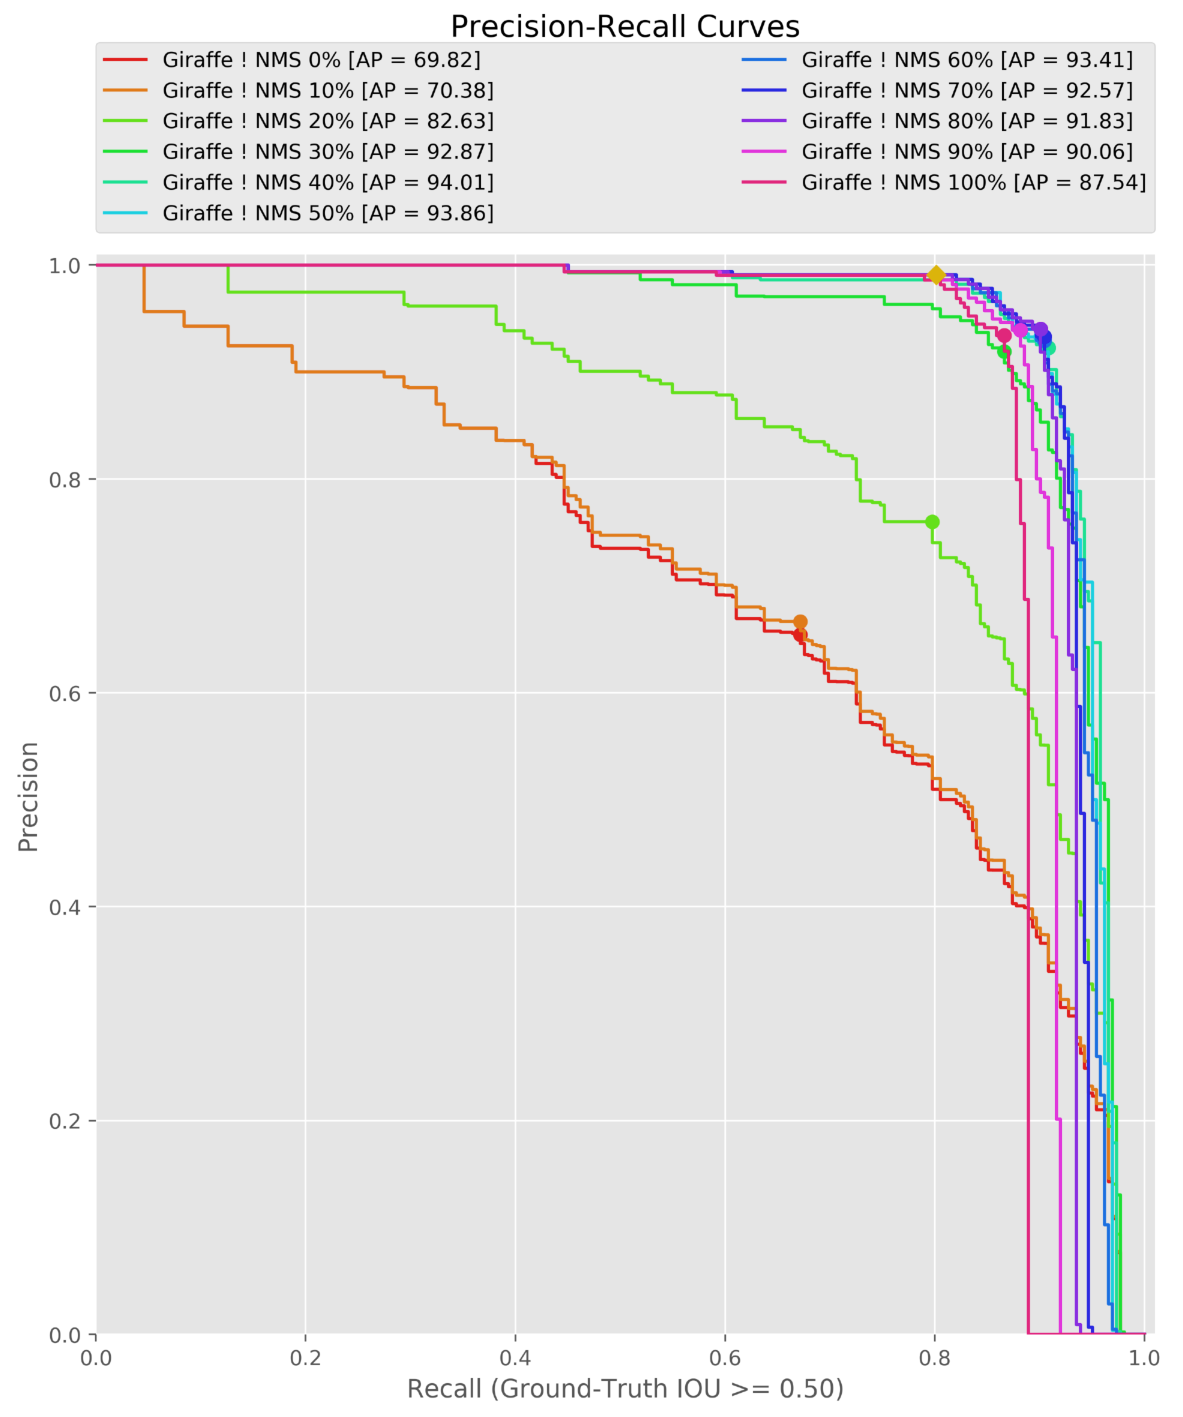
\includegraphics[width=0.45\linewidth]{resources/ggr2-!giraffe-lightnet-localizer-precision-recall-50.pdf}
    \end{center}
    \caption{The precision-recall performance curves for the localizer during the GGR-18 photographic censusing rally.  The performance of the localizer on zebra (left) and giraffe (right) AoIs for the GGR-18.  The NMS threshold that achieved the highest precision-recall AP for each species was chosen, followed by the operating point that was the closest to the top-right corner, balancing precision and recall for the highest area of AP.  Coincidentally, both species had the best performance with a NMS threshold of 40\% overlap and -- approximately for both species -- a best operating point at 0.4 for the detection confidence.}
    \label{fig:performance-localizer-ggr}
\end{figure}

The whole-image classifier (see Section~\ref{sec:wic}) and localizer were trained with an annotated subset of bounding boxes with their species labels.  The precision-recall performance curves of AoI detections can be seen in Figure~\ref{fig:performance-localizer-ggr} for Gr\'evy's zebra (left) and reticulated giraffe (right).  The figures show varying levels of non-maximum suppression (NMS) applied on the output detections, both achieving an AP of at least 94\% for their best respective configurations.  The next step was having reviewers add viewpoint assignments to each animal (across the cardinal and sub-cardinal eight directions) for training the annotation classifier.  The bounding boxes with species assignments also provided sufficient training data for training the coarse foreground-background segmentation classifier.  Lastly, reviewers were asked to annotate the AoIs in the image to provide training data for the AoI classifier.  The human-curated data was used to bootstrap all of the core detection pipeline components and was then applied to the remaining 90\% of the collected data.

\begin{figure}[!t]
    \begin{center}
        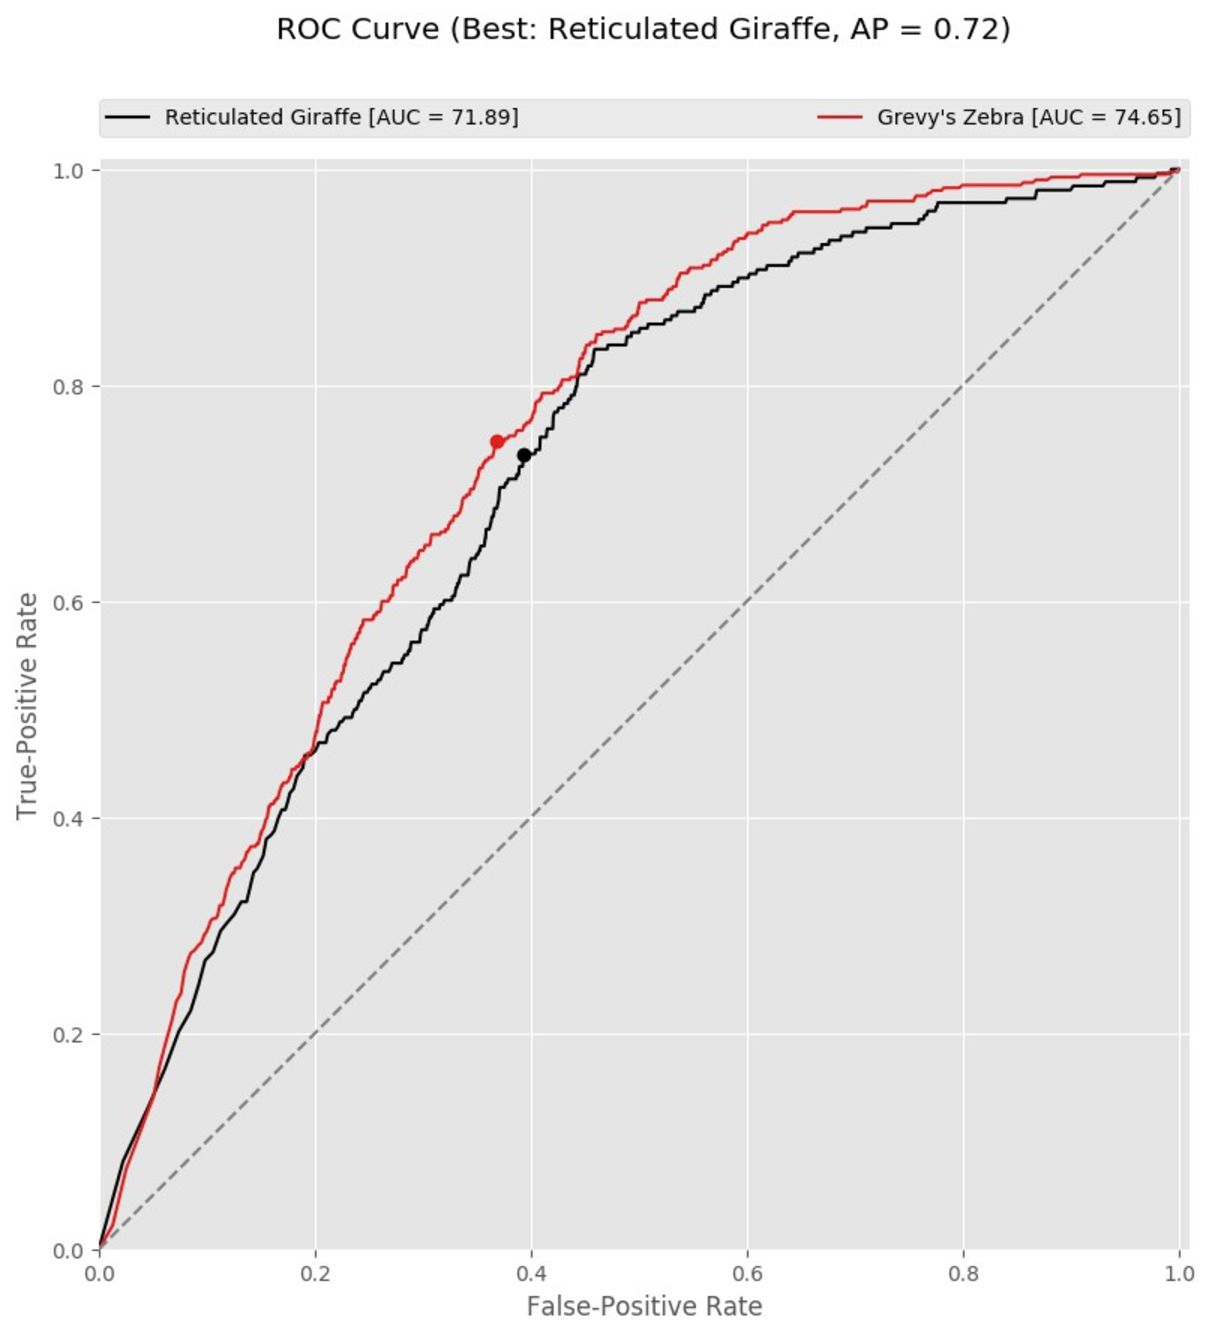
\includegraphics[width=0.6\linewidth]{resources/aoi2-precision-recall-roc-ggr2.pdf}
    \end{center}
    \caption{The ROC performance curves for the AoI component during the GGR-18 photographic censusing rally.  The AoI classifier was trained to predict the majority decided AoI flags on each annotation annotated from the 5,000 training image set for the GGR-18.}
    \label{fig:performance-aoi-ggr}
\end{figure}

The AoI classifier has a classification accuracy of 76.49\% on average between the two species, indicating moderate success in eliminating apparent background sightings.  The ROC curves of the re-trained classifier can be viewed in Figure~\ref{fig:performance-aoi-ggr}.  The number of identifiable annotations collected for each species can be seen in Table~\ref{table:stats}.  At the time of processing the annotations for the GGR-18, this AoI filtering model was deemed to be inadequate.  The failure modes for AoI were significant and varied enough that it suggested a new concept for identifiability was needed.  The concept of Census Annotations and Census Annotation Regions (see Chapter~\ref{chapter:ca}) were partially motivated by this AoI classification performance during the GGR-18.  These new components are meant to be a drop-in replacement for AoI in future censusing events, as will be demonstrated below in Section~\ref{sec:ggr18-culminating}.

\subsubsection{Animal ID Curation}

There were three primary challenges with using the Graph ID algorithm for ID curation during the GGR-16 and GGR-18: 1) it was still dependent on large amounts of human effort for review 2) its internal ID ranking process (HotSpotter) took a long time to compute for large databases and 3) it had specific implementation inefficiencies that made it hard to fit into memory.  The basic building block of the Graph ID algorithm is the ranking results, without which the curation process is aimless and has quadratic complexity.  The algorithm uses the ranked list to prioritize which matches are sent to human reviewers and automated decision algorithms, representing the largest source of pairs during the analysis.  Furthermore, the total number of reviews will be influenced by the parameters of the ranking algorithm (e.g., GGR-18 returned the top five matches for each query annotation).  Some of the ranked matches are intentionally discarded for being poor spatial candidates; some are discarded for failing to pass a score threshold; some are bi-directional duplicates (i.e., A matched B and B matched A, so one match pair is discarded).  For example, for 11,916 Census Annotation Regions and a ranked list configuration that returns the top-10 matches (allowing twice as many potential matches as top-5), the HotSpotter algorithm suggests 67,247 total matches.  The resulting ranked list is passed to the VAMP automated verifier, which automatically decides pairs above a scores threshold (as specified by held-out validation data).  Any match that falls below the threshold is provided to a human for a decision.

The verifier score threshold is not the only way for reviews to be added to the queue of pairs that need a decision from a human reviewer.  When the Graph ID algorithm identifies an inconsistency, it immediately adds additional annotation pairs into the queue to find the problem.  Ideally, the top of the human review queue (and the first to be provided to a reviewer) is the match that is actively blocking the ID curation algorithm.  Unfortunately, this means that the review process is restrictively iterative.  Worse, the processing between each annotation is non-deterministic, meaning that the Graph ID algorithm could take an indeterminate amount of time before providing the next match to review to a human.  Herein lies a dilemma: we wish to 1) provide a match to a reviewer such that the ID curation algorithm can resume\footnote{Refer to~\cite{crall_identifying_2017} for specific details on Graph ID and its phase-based workflow.} and 2) never run out of relevant reviews to provide to the active reviewers.  For the GGR-16 and GGR-18 processing, it took a team of around a dozen reviewers working concurrently against an ever-updating set (n=500) of candidate matches to review.  Even with advanced and accurate machine learning methods for detection, feature description, ranking, and pairwise verification, it still took months of full-time analysis to review comprehensively.

For each annotation, approximately 3-4 human or automated reviews were required (top-5) for the animal ID database to be consistent.  For example, the GGR-18 analysis incorporated 10,044 Gr\'evy's zebra and 4,018 reticulated giraffe annotations and required 35,608 total pairwise reviews.  Exactly 18,556 reviews were performed by a human reviewer (52.1\%) during GGR-18, which indicates that -- optimistically -- at least 1.5 human reviews per annotation are required on average.  Thus, the process used by the GGR-16 and GGR-18 events does not represent a scalable solution to large-scale photographic censusing.  What is needed is 1) an order-of-magnitude reduction in the amount of human involvement in photographic censusing and 2) non-blocking curation algorithms that do not require highly iterative workflows.  The GGR-16 and GGR-18 events did not benefit from Census Annotation Regions and LCA at the time, and their respective ID curations were mainly performed by hand.  Luckily, as we have seen, the ID databases for both events converged and can be used as a comparative baseline for future algorithm development.  The following sub-section provides some implementation details on how the memory constraints of the Graph ID algorithm were mitigated.  The reader can safely skip to Section~\ref{sec:demographics} to review the next step of the photographic censusing procedure on demographics and quality checks.

\subsubsection{Implementation Details for Tree-based Graph ID Curation}

\begin{figure}[!t]
    \begin{center}
        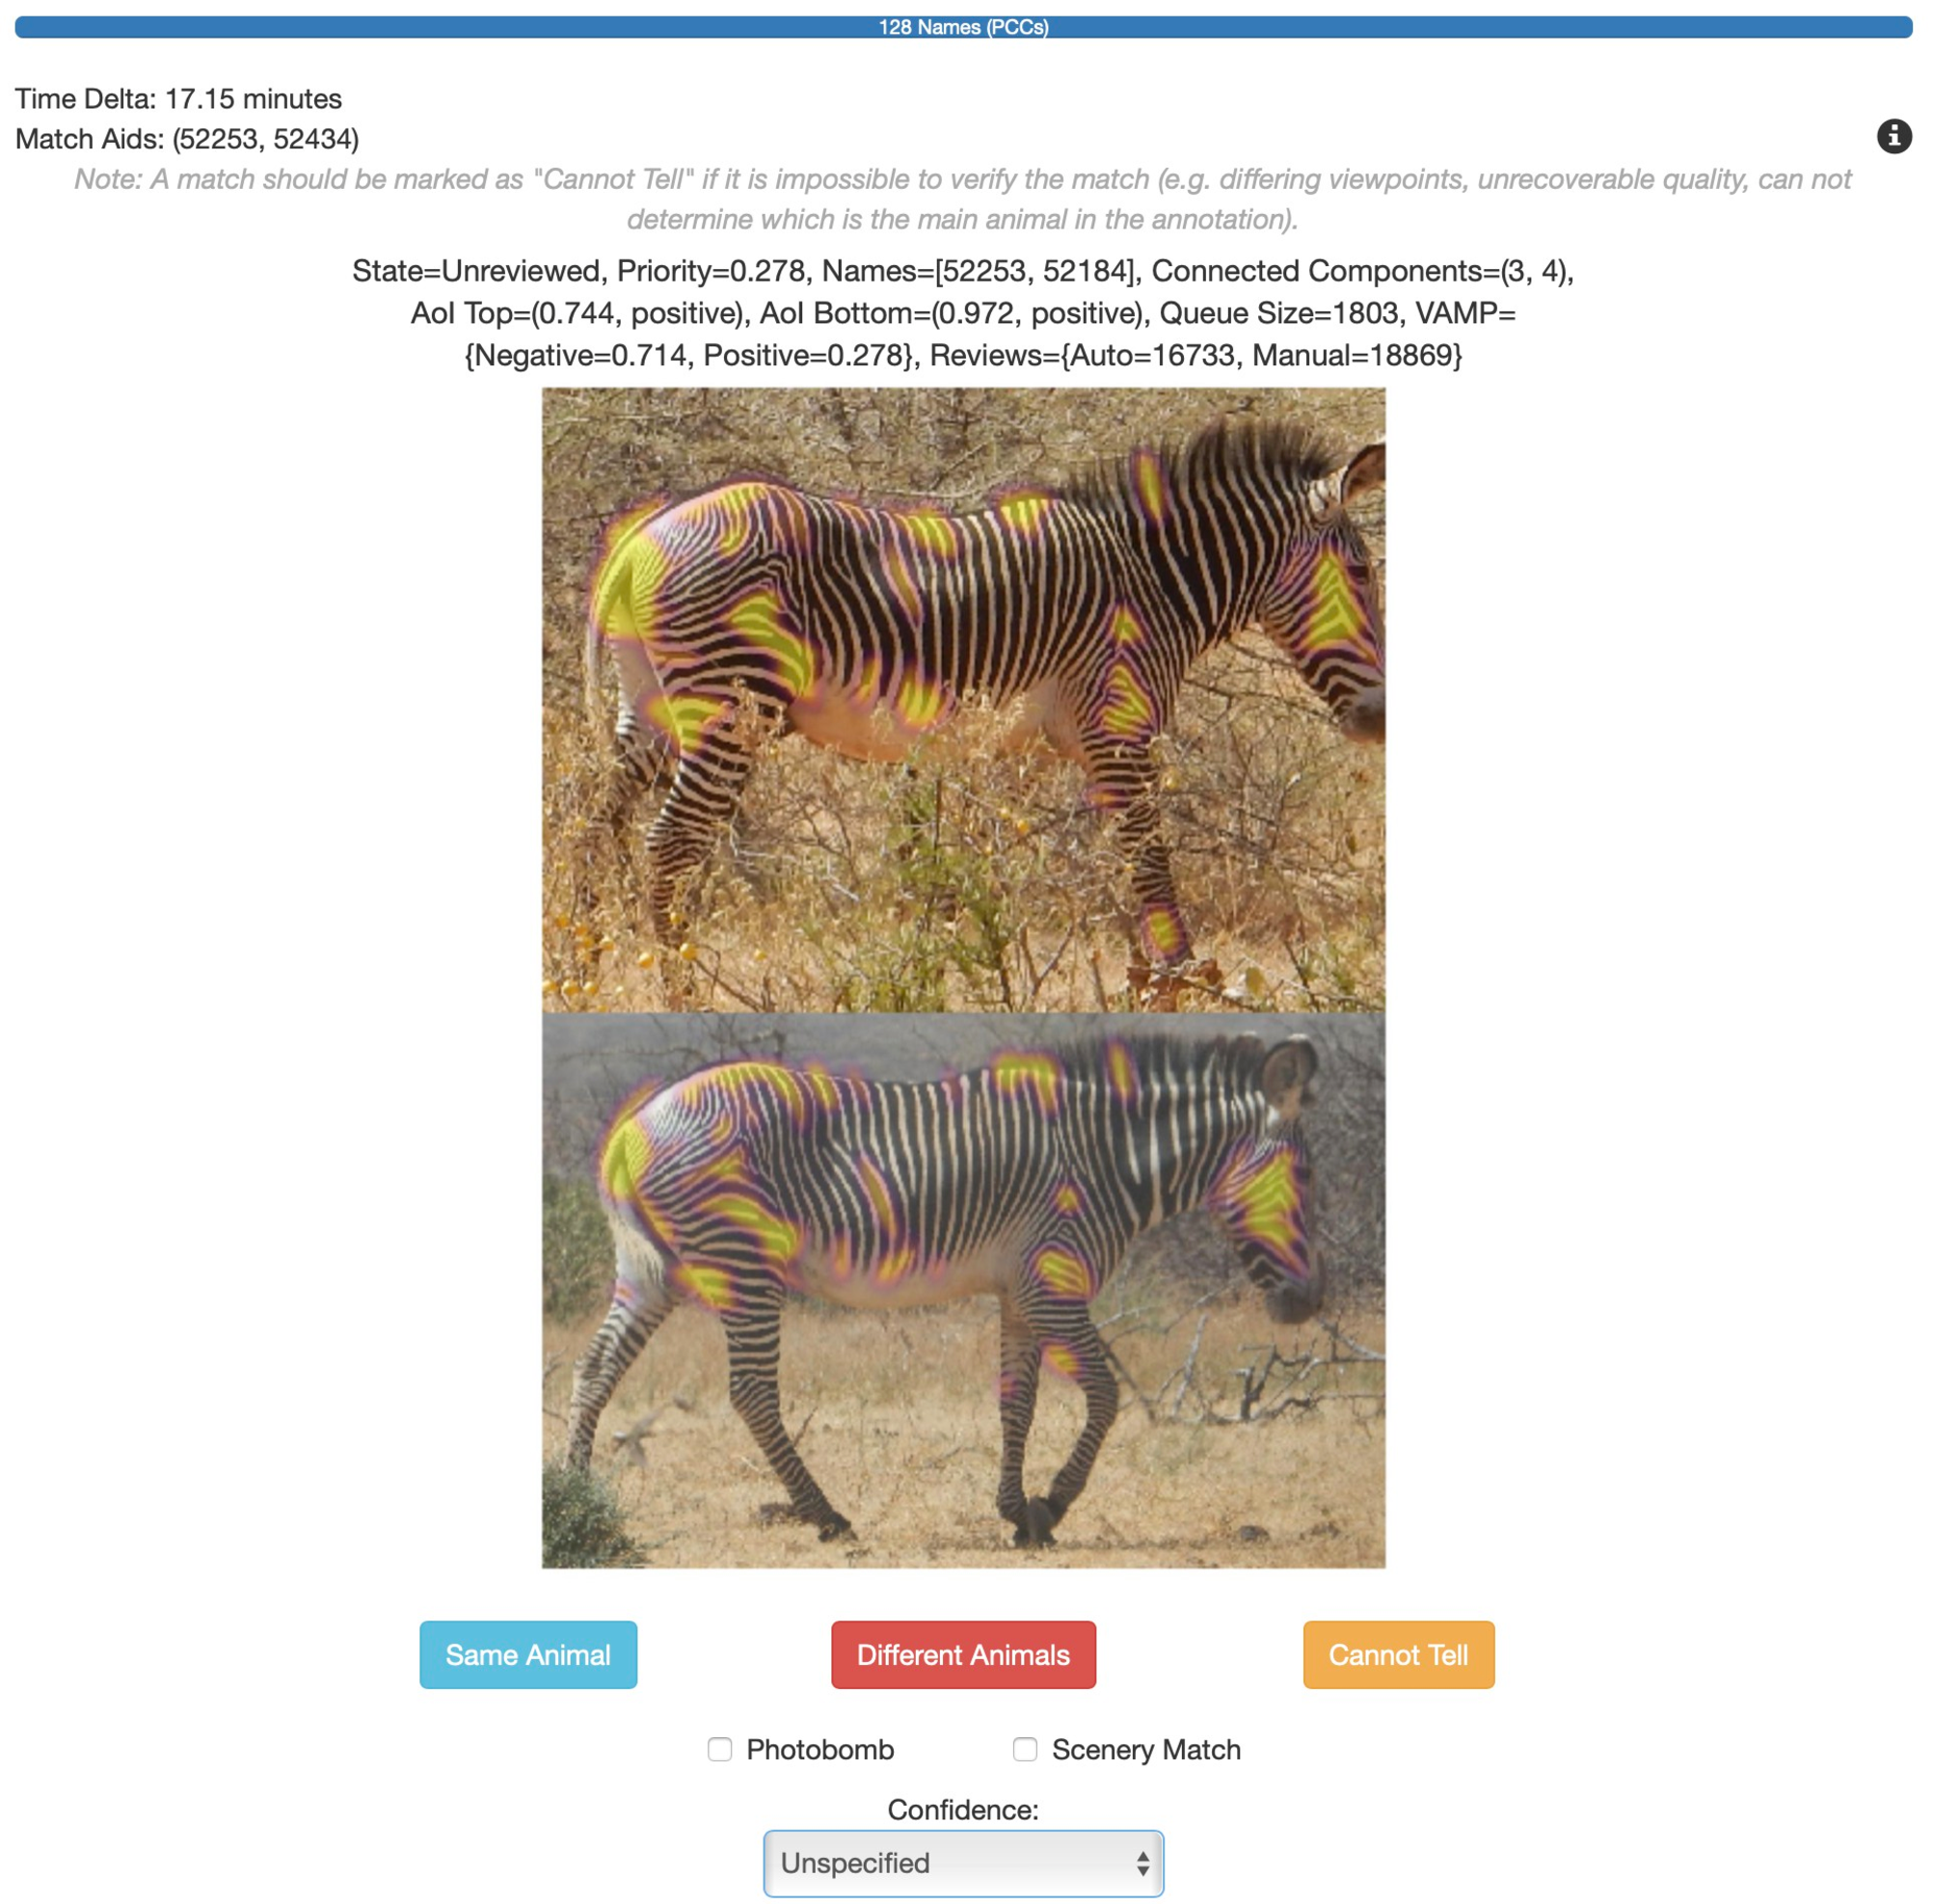
\includegraphics[width=0.85\linewidth]{resources/graph_algorithm.pdf}
    \end{center}
    \caption{An image of the web interface for reviewing matched annotation pairs.  The Graph ID algorithm suggests an iterative list of matches for review by humans.  We extend the base algorithm to make it asynchronous and allow multiple web-based reviewers to make decisions concurrently.  This match shows an example of a \texttt{negative} match.}
    \label{fig:graph-algorithm}
\end{figure}

The selected annotations for ID from the detection pipeline were partitioned into a binary tree (four levels for zebras and three levels for giraffes) to more efficiently control the ID curation process.  This structure allowed different parts of the ID database to be worked on simultaneously by the same pool of reviewers.  Each leaf of the tree was balanced such that there existed roughly 1,000 annotations, with annotations taken by the same car automatically grouped.  A reviewer was then dispatched to work on one of the 16 (or 8) leaves to review whatever matches were ready for human review.  If the review queue for a given leaf was empty (e.g., when processing in the background to generate new reviews), we provided the reviewer with a different leaf waiting for a human decision.  The interface (Figure~\ref{fig:graph-algorithm}) provides the reviewer with two animal sightings (top and bottom) and a heat-map for the suggested correspondences.  Once all of the leaves for a given level had converged, they were merged in pairs of two.  The process was then restarted, comparing leaves that were twice as large as the previous round.  The curation continued and worked up the binary tree towards the root, which contained all the annotations.  As the final matching was performed on the root, the rate of finding new animals slowed.  By the time the last two leaves were merged into a single root, the vast majority of the reviews had already been completed.  The analysis was terminated when there were no more merges and split cases after a specified period.

\subsubsection{Demographics \& Quality Checks} \label{sec:demographics}


\begin{figure}[!t]
    \begin{center}
        \begin{tabular}{ccc}
            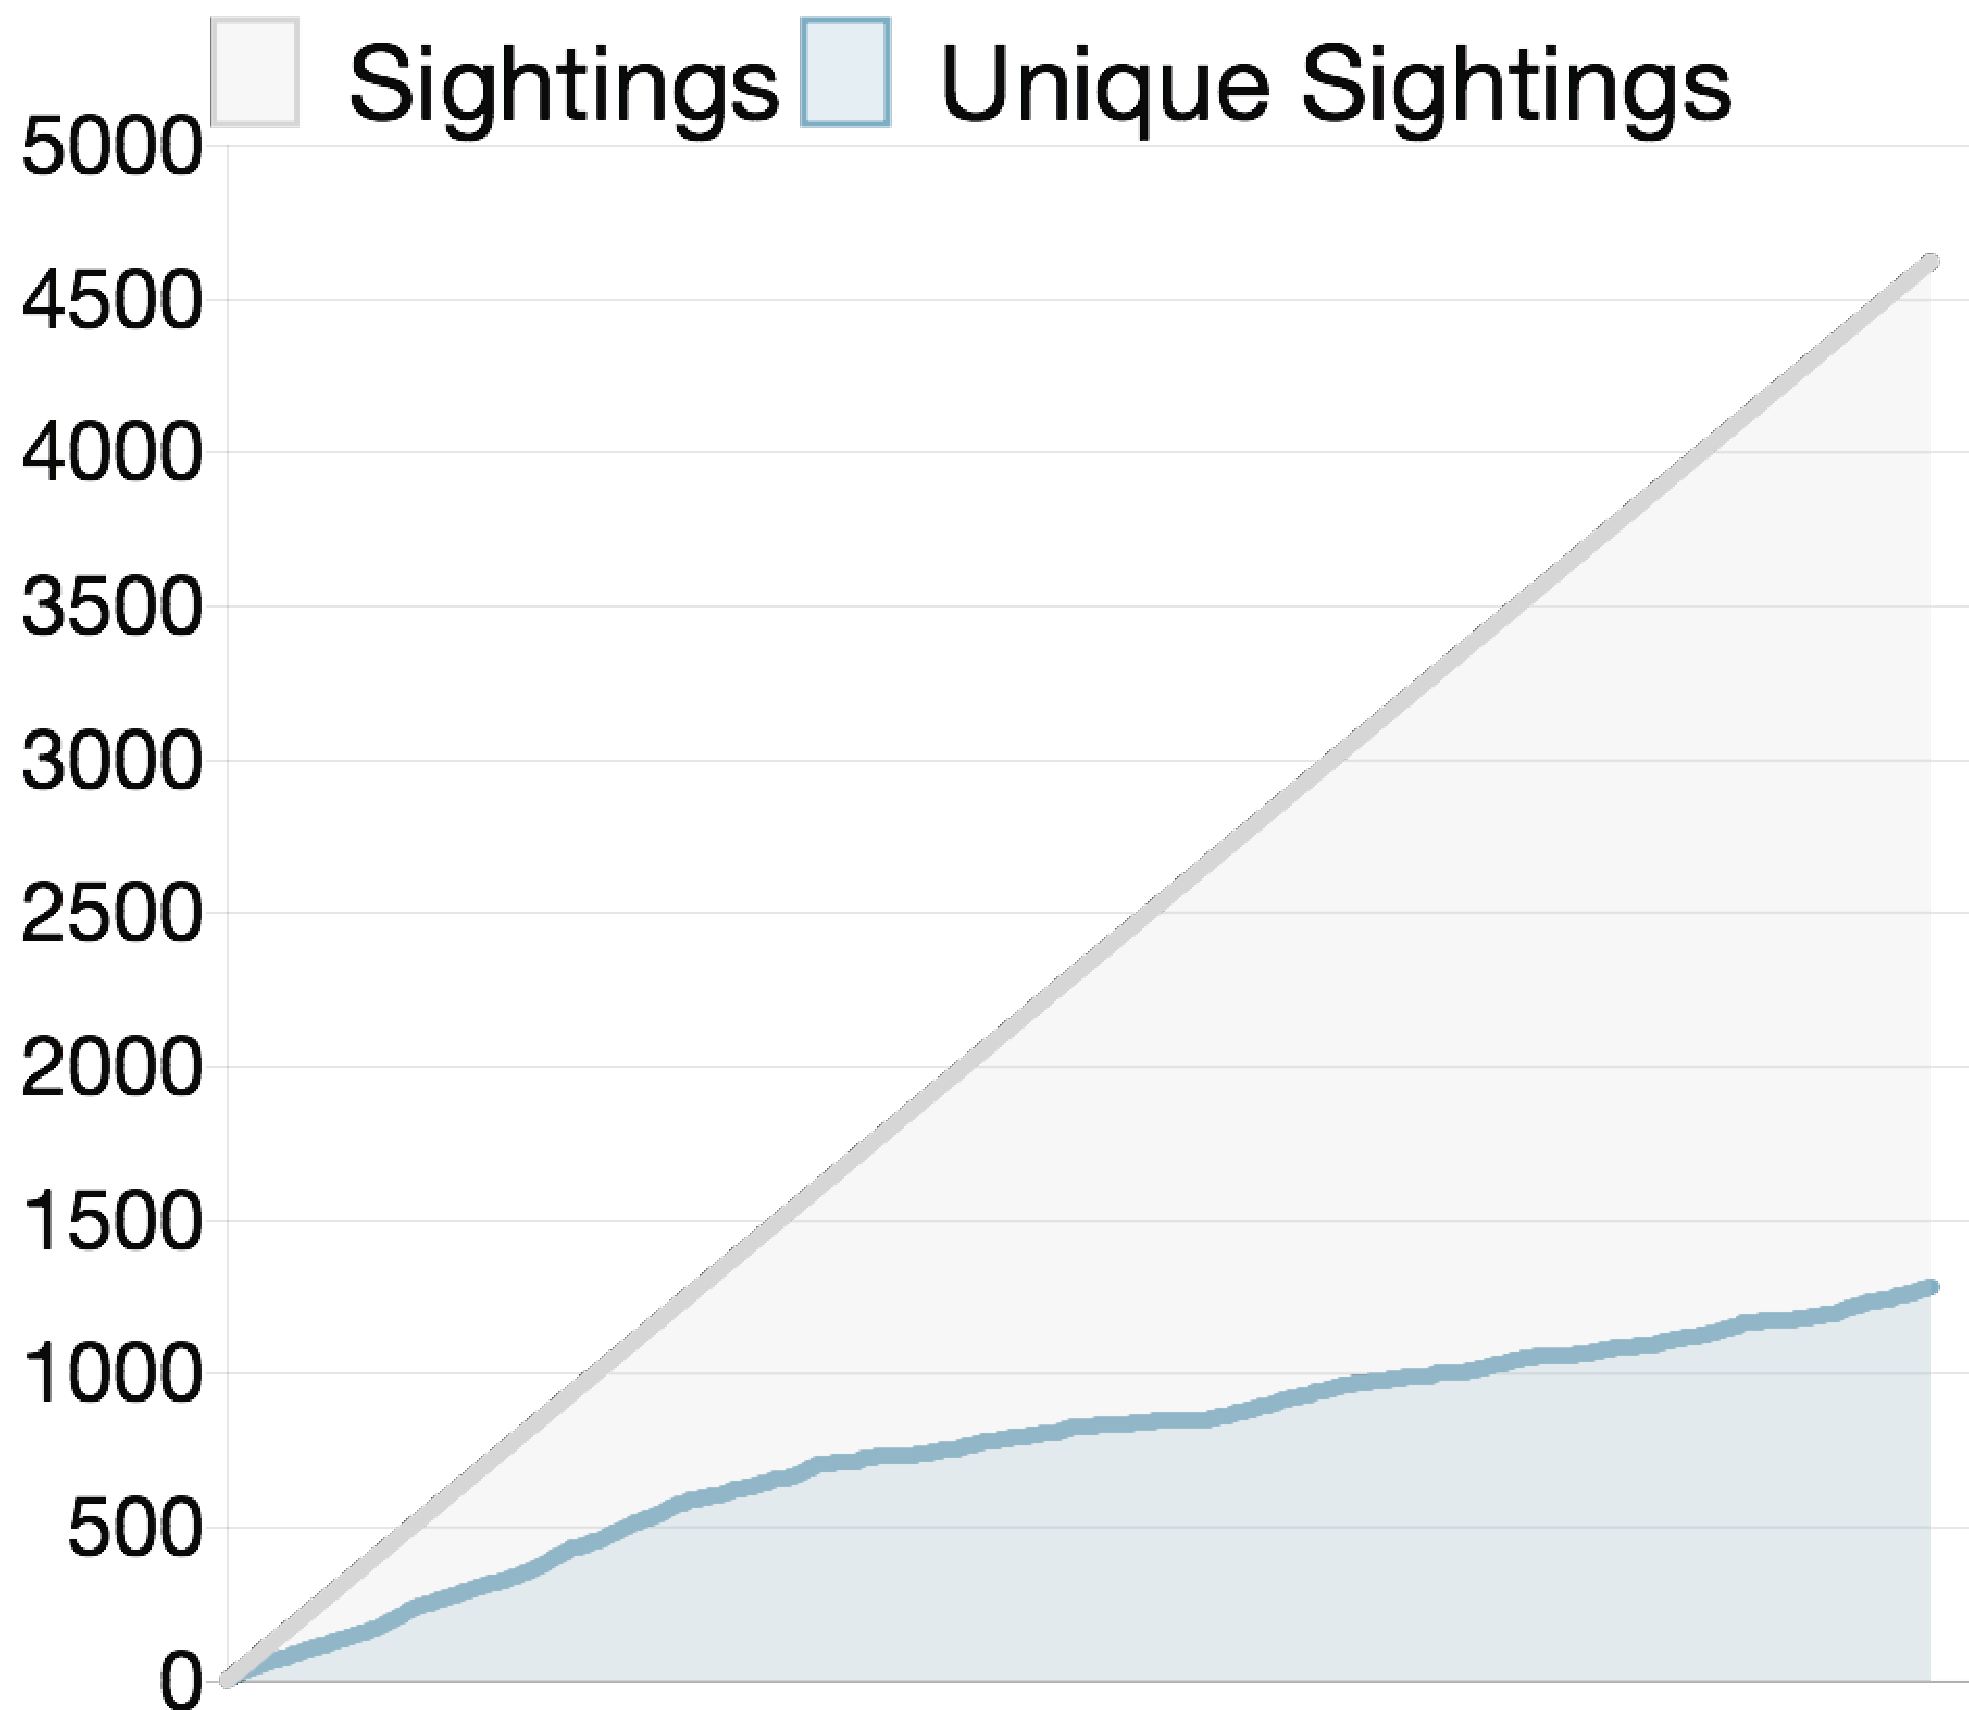
\includegraphics[width=0.32\linewidth]{resources/convergence-gzgc.pdf} &
            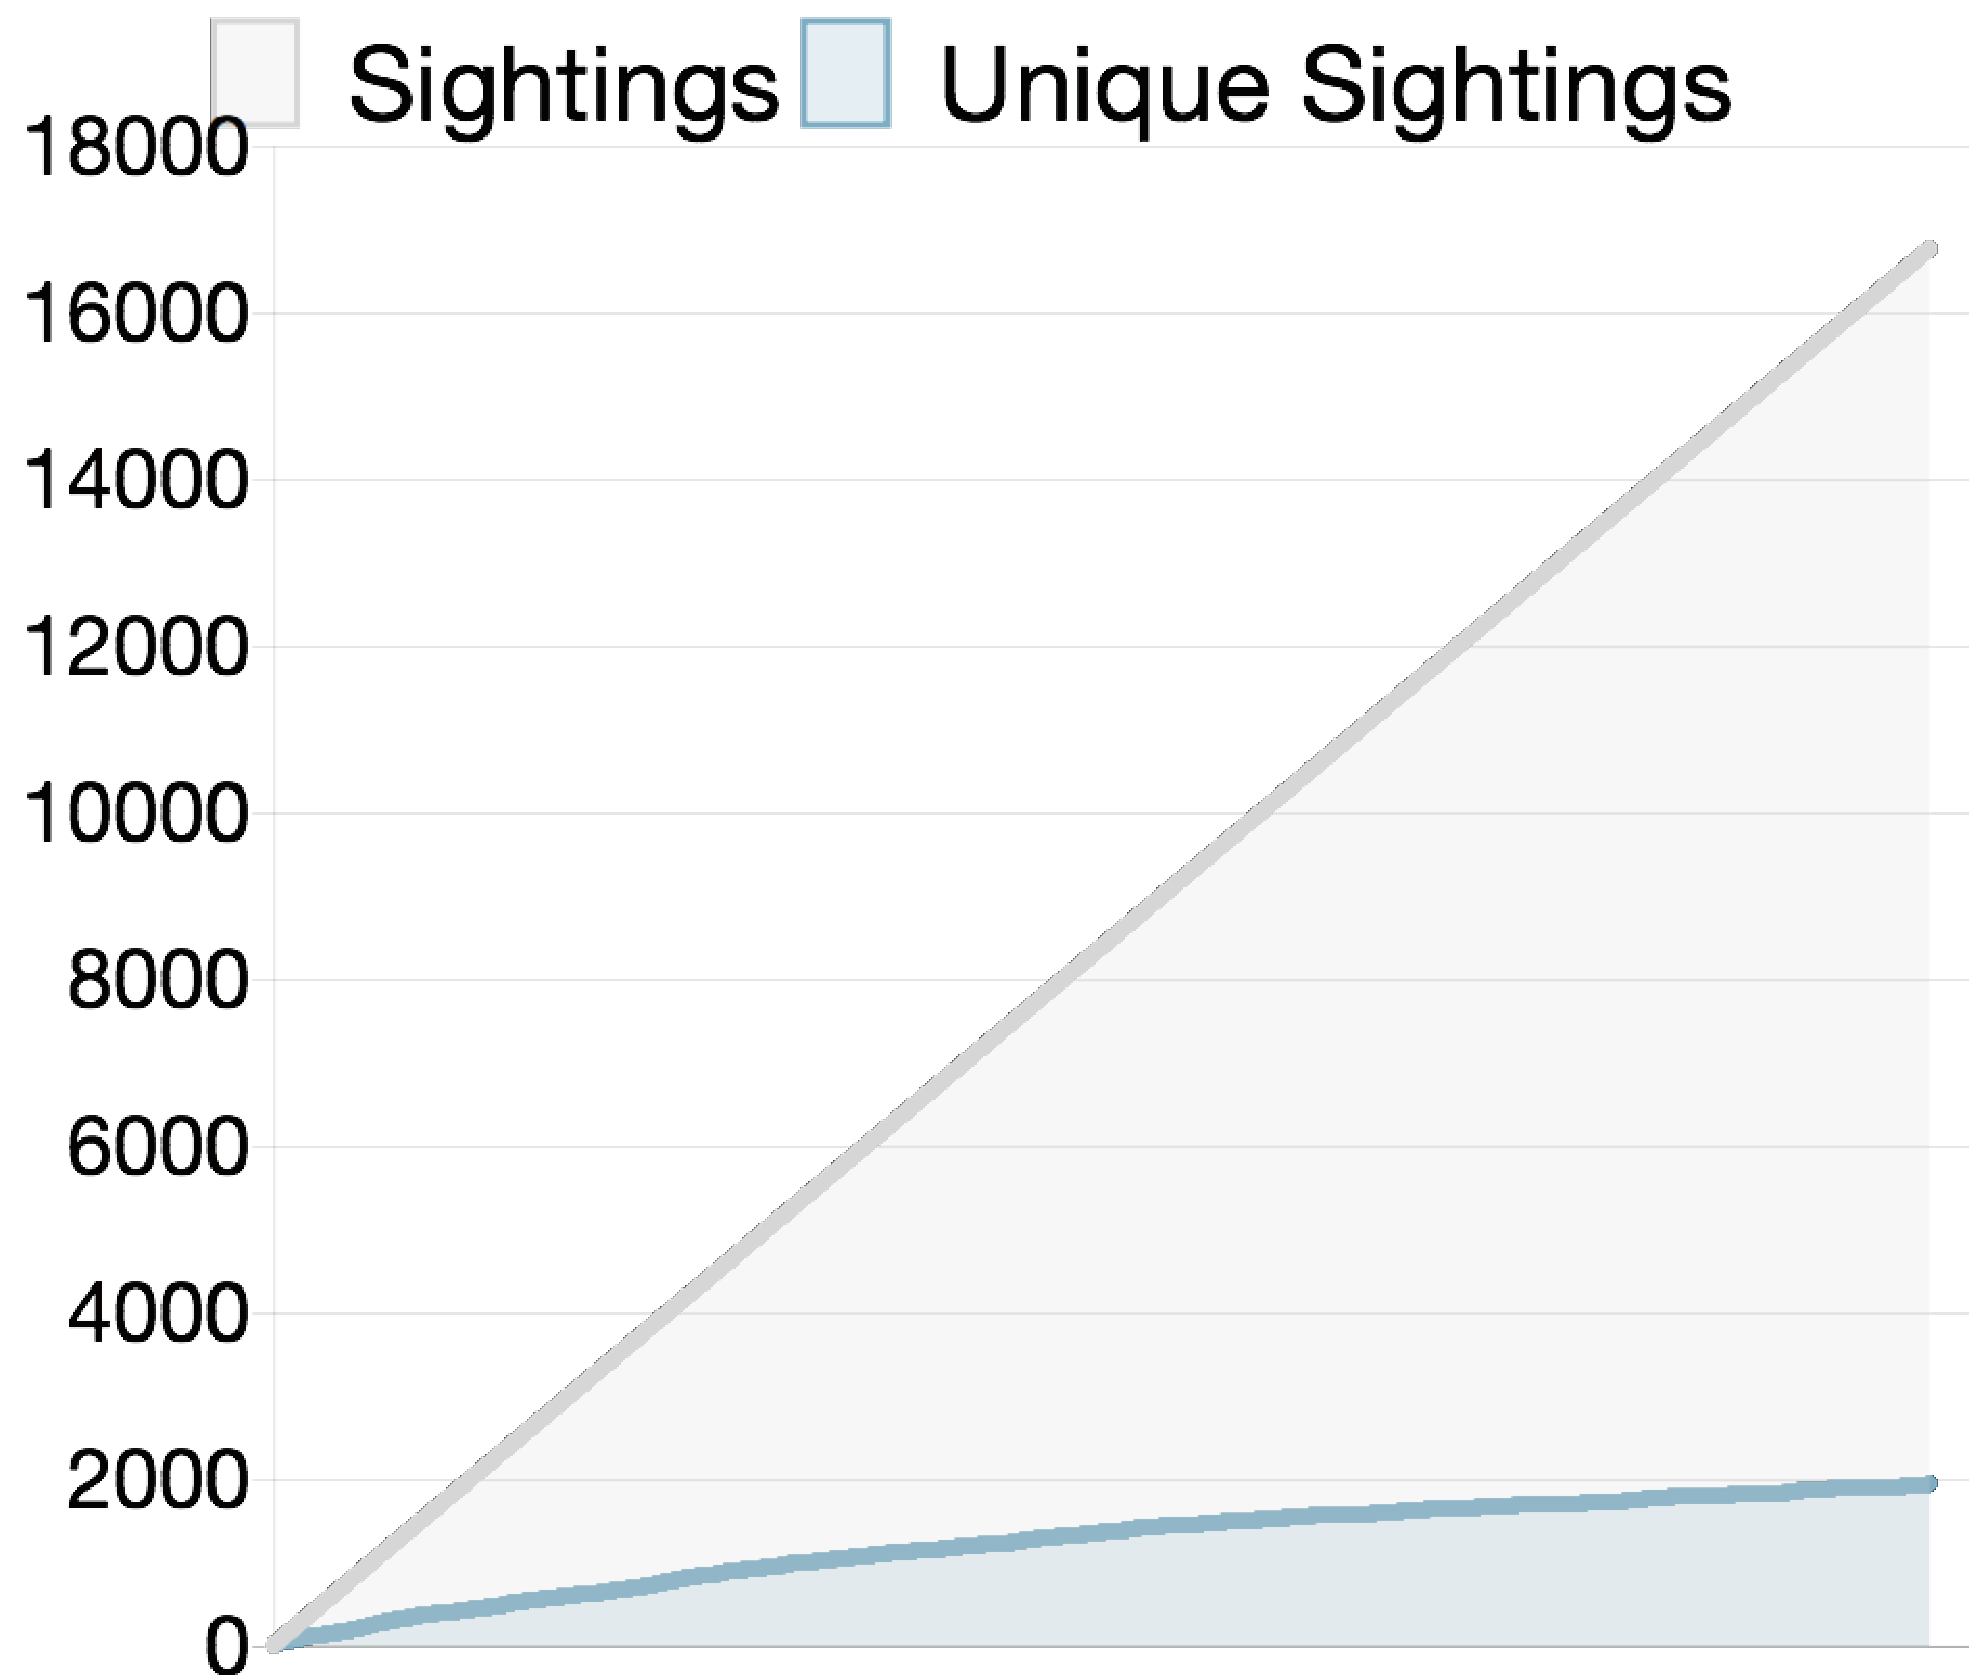
\includegraphics[width=0.32\linewidth]{resources/convergence-ggr.pdf}  &
            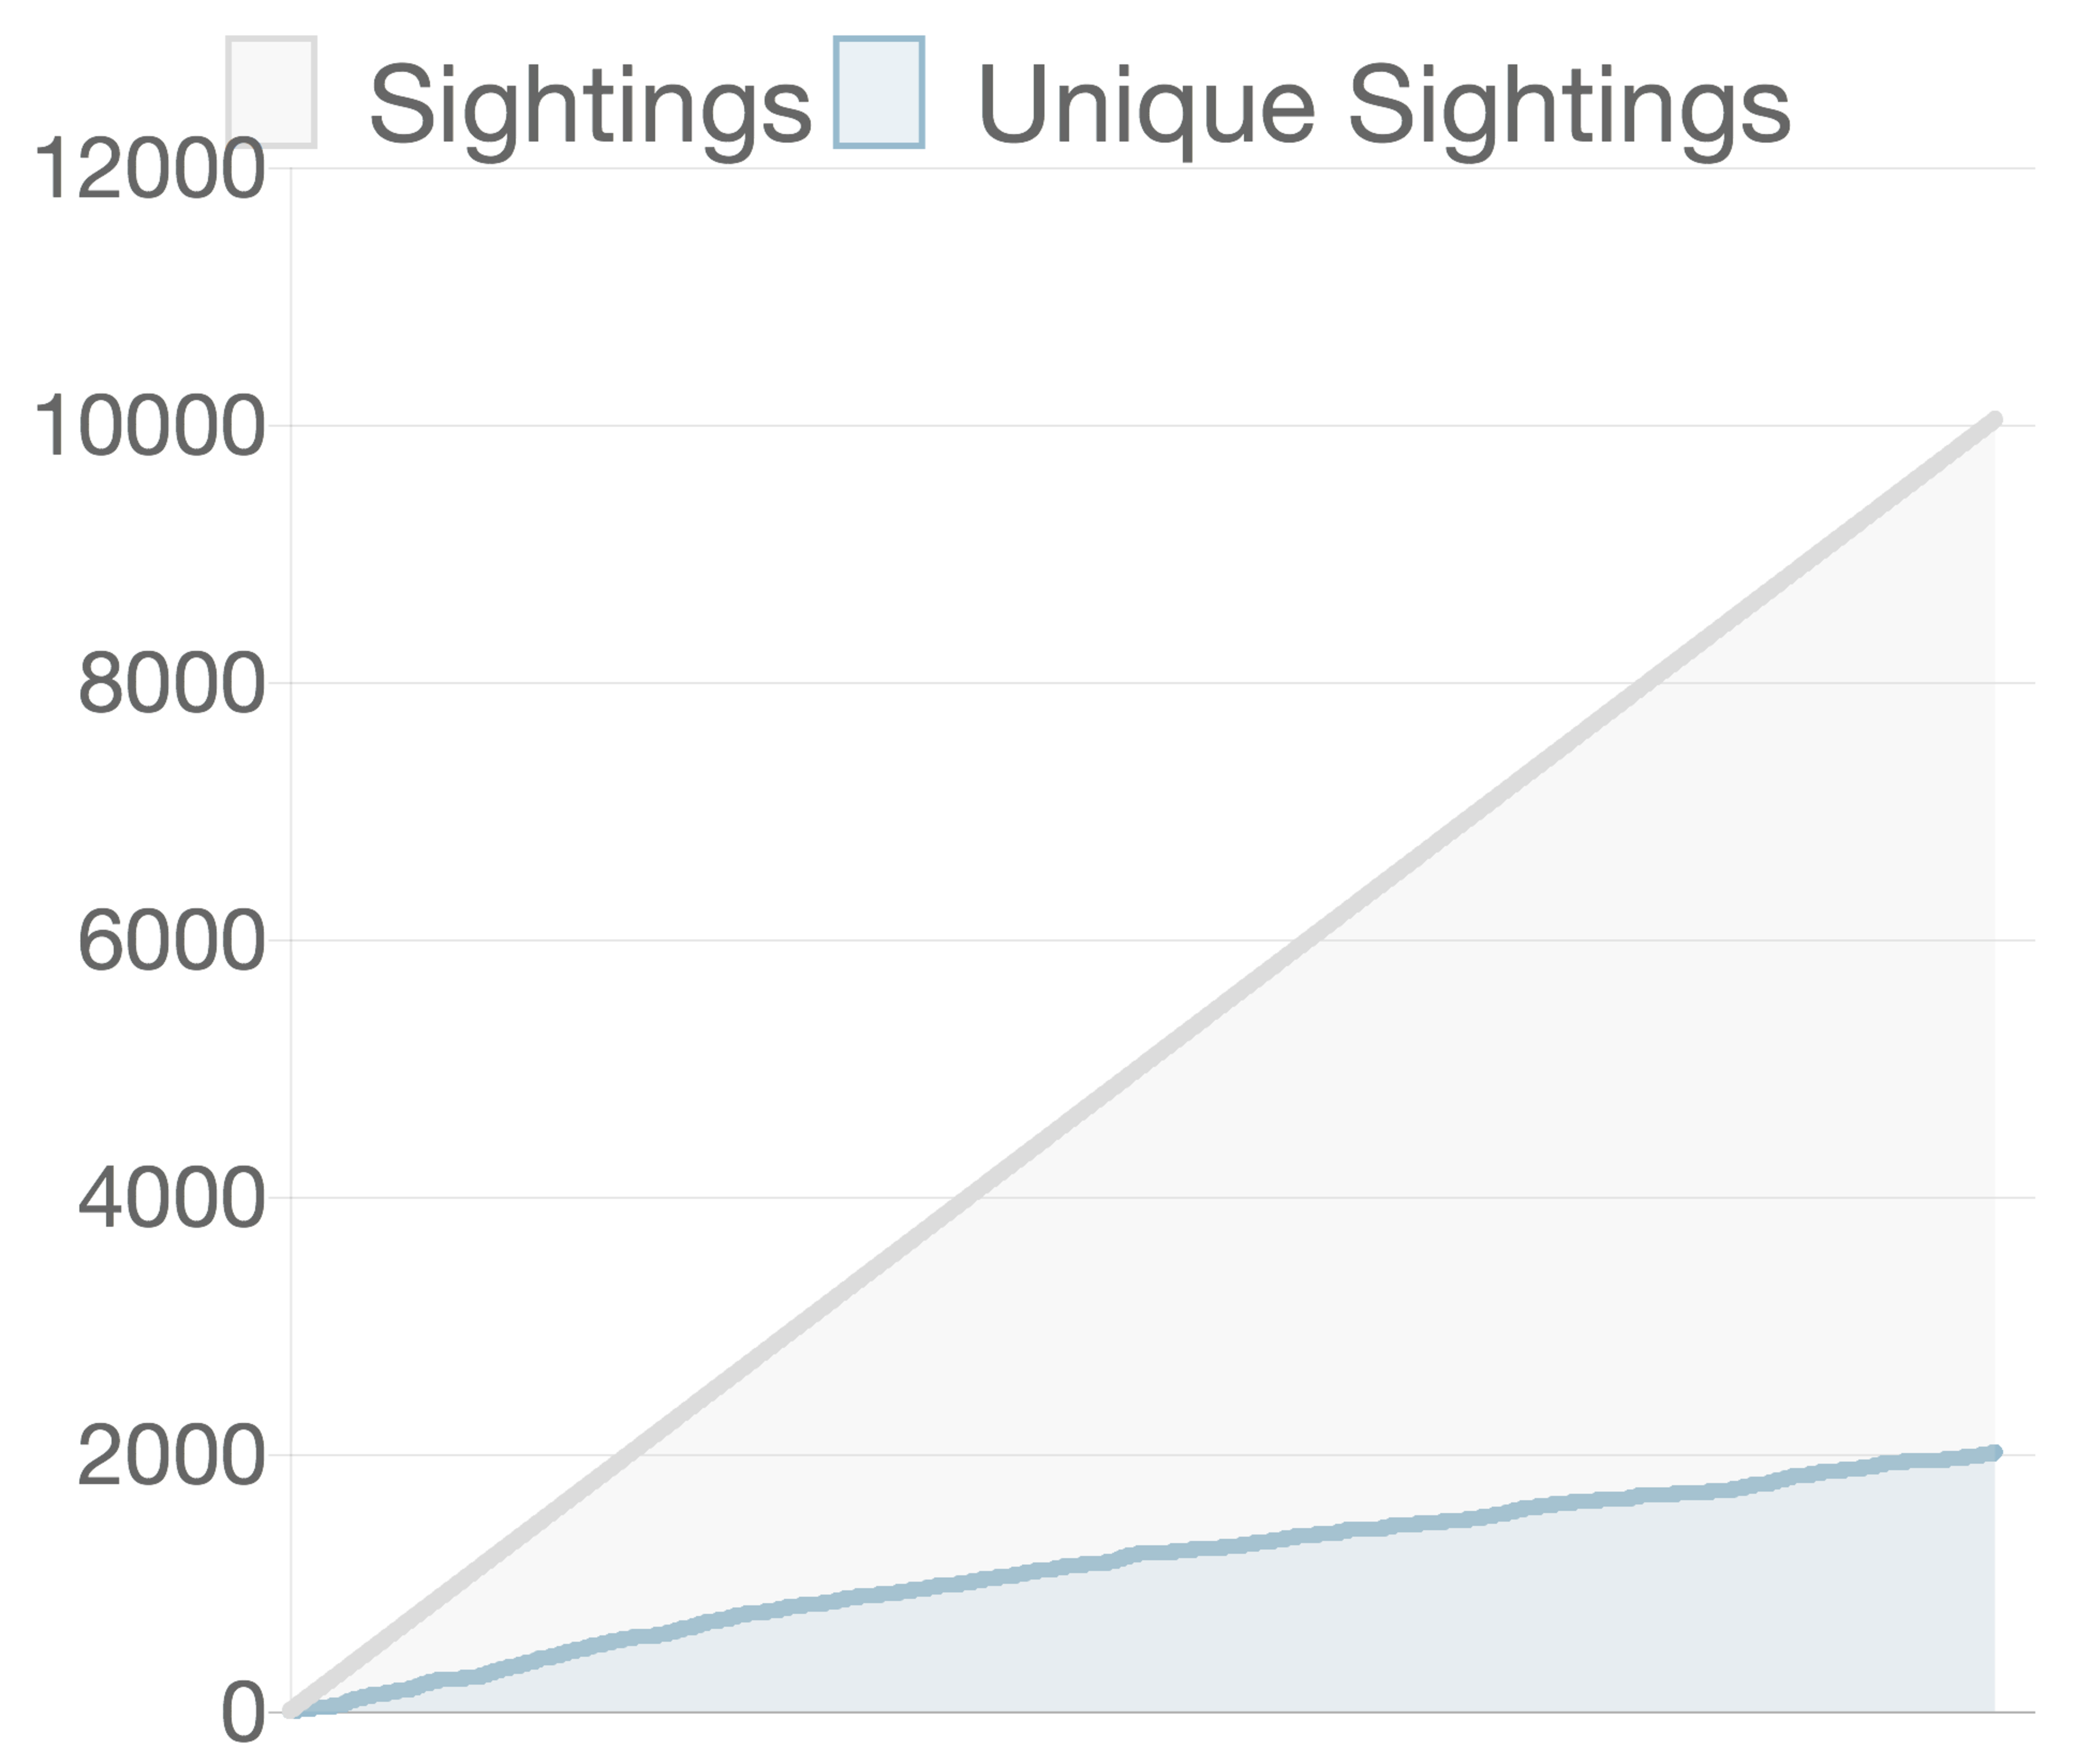
\includegraphics[width=0.32\linewidth]{resources/convergence-ggr18.pdf}  \\
            \textbf{GZGC}                                                          &
            \textbf{GGR-16}                                                        &
            \textbf{GGR-18}
        \end{tabular}
    \end{center}
    \caption{A plot of the identification convergence rates for the GZGC, GGR-16, and GGR-18 photographic censusing rallies.  The convergence of the identification algorithm during the GZGC~\cite{parham_photographic_2015} (left), the GGR-16 (middle), and the GGR-18 (right).  The x-axis shows all collected photographs in chronological order and the y-axis shows the number of sightings against new sightings.  The x-axis is the same scale as the y-axis.  As photos are processed over time, the rate of new sightings decreases.  The smaller slope of the GGR rallies indicate that the rate of resightings for the GGR censusing events were higher than the GZGC.  [GZGC \& GGR-16] \copyright 2017 AAAI. Reprinted, with permission, from: J. Parham, J. Crall, C. Stewart, T. Berger-Wolf, and D. I. Rubenstein, ``Animal population censusing at scale with citizen science and photographic identification,'' in \textit{AAAI Spring Symp.}, Palo Alto, CA, USA, Jan. 2017, pp. 37–44.}
    \label{fig:convergence}
\end{figure}

Once the ID curation was complete, ecologists were asked to manually annotate age and sex information for each animal ID in the database.  The reviewer was presented with all of the annotations for a given individual animal to make a more accurate decision (e.g., to browse for unambiguous photographs of genitalia).  The review of age and sex also allows for an error checking method, where any cross-gender or cross-age matching mistakes were flagged and corrected.  The reader is referred to the field reports~\cite{berger-wolf_great_2016,rubenstein_state_2018,rubenstein_great_2015} for a breakdown on the demographics during the GGR-16 and GGR-18 along with discussion on population stability.

Another name-based check is to ensure travel constraints through GPS and time EXIF metadata.  For example, an animal that appeared to travel too far in a short period was marked as a potentially lousy ID with multiple animals and sent for additional review.  For the GGR-16 and GGR-18 events, a global constraint of 10 km/h was applied to all sightings of Gr\'evy's zebra and reticulated giraffe.  This speed check identified a handful of annotations that were improperly merged into the same ID and were manually fixed by splitting the ID into two (or more) individual animals.

The animal IDs are then combined with their image's date/timestamps to determine when and where an animal was seen.  Knowing the number of sightings on day 1 only, day 2 only, and resightings between both days allow a Lincoln-Petersen estimate to be calculated as in a traditional mark-recapture study (Table~\ref{table:stats}). In addition, embedded GPS meta-data -- and knowing the camera and car a photograph originates from -- can be used to analyze the spatial and temporal distributions of the data and the distributions by car and photographer.  The result is a final list of the named animals with age and sex information, which can then be compared to previous years to develop a list of deaths, births, migration patterns, and other ecological insights.

\subsubsection{Convergence \& Sighting Distribution}

\begin{figure}[!t]
    \begin{center}
        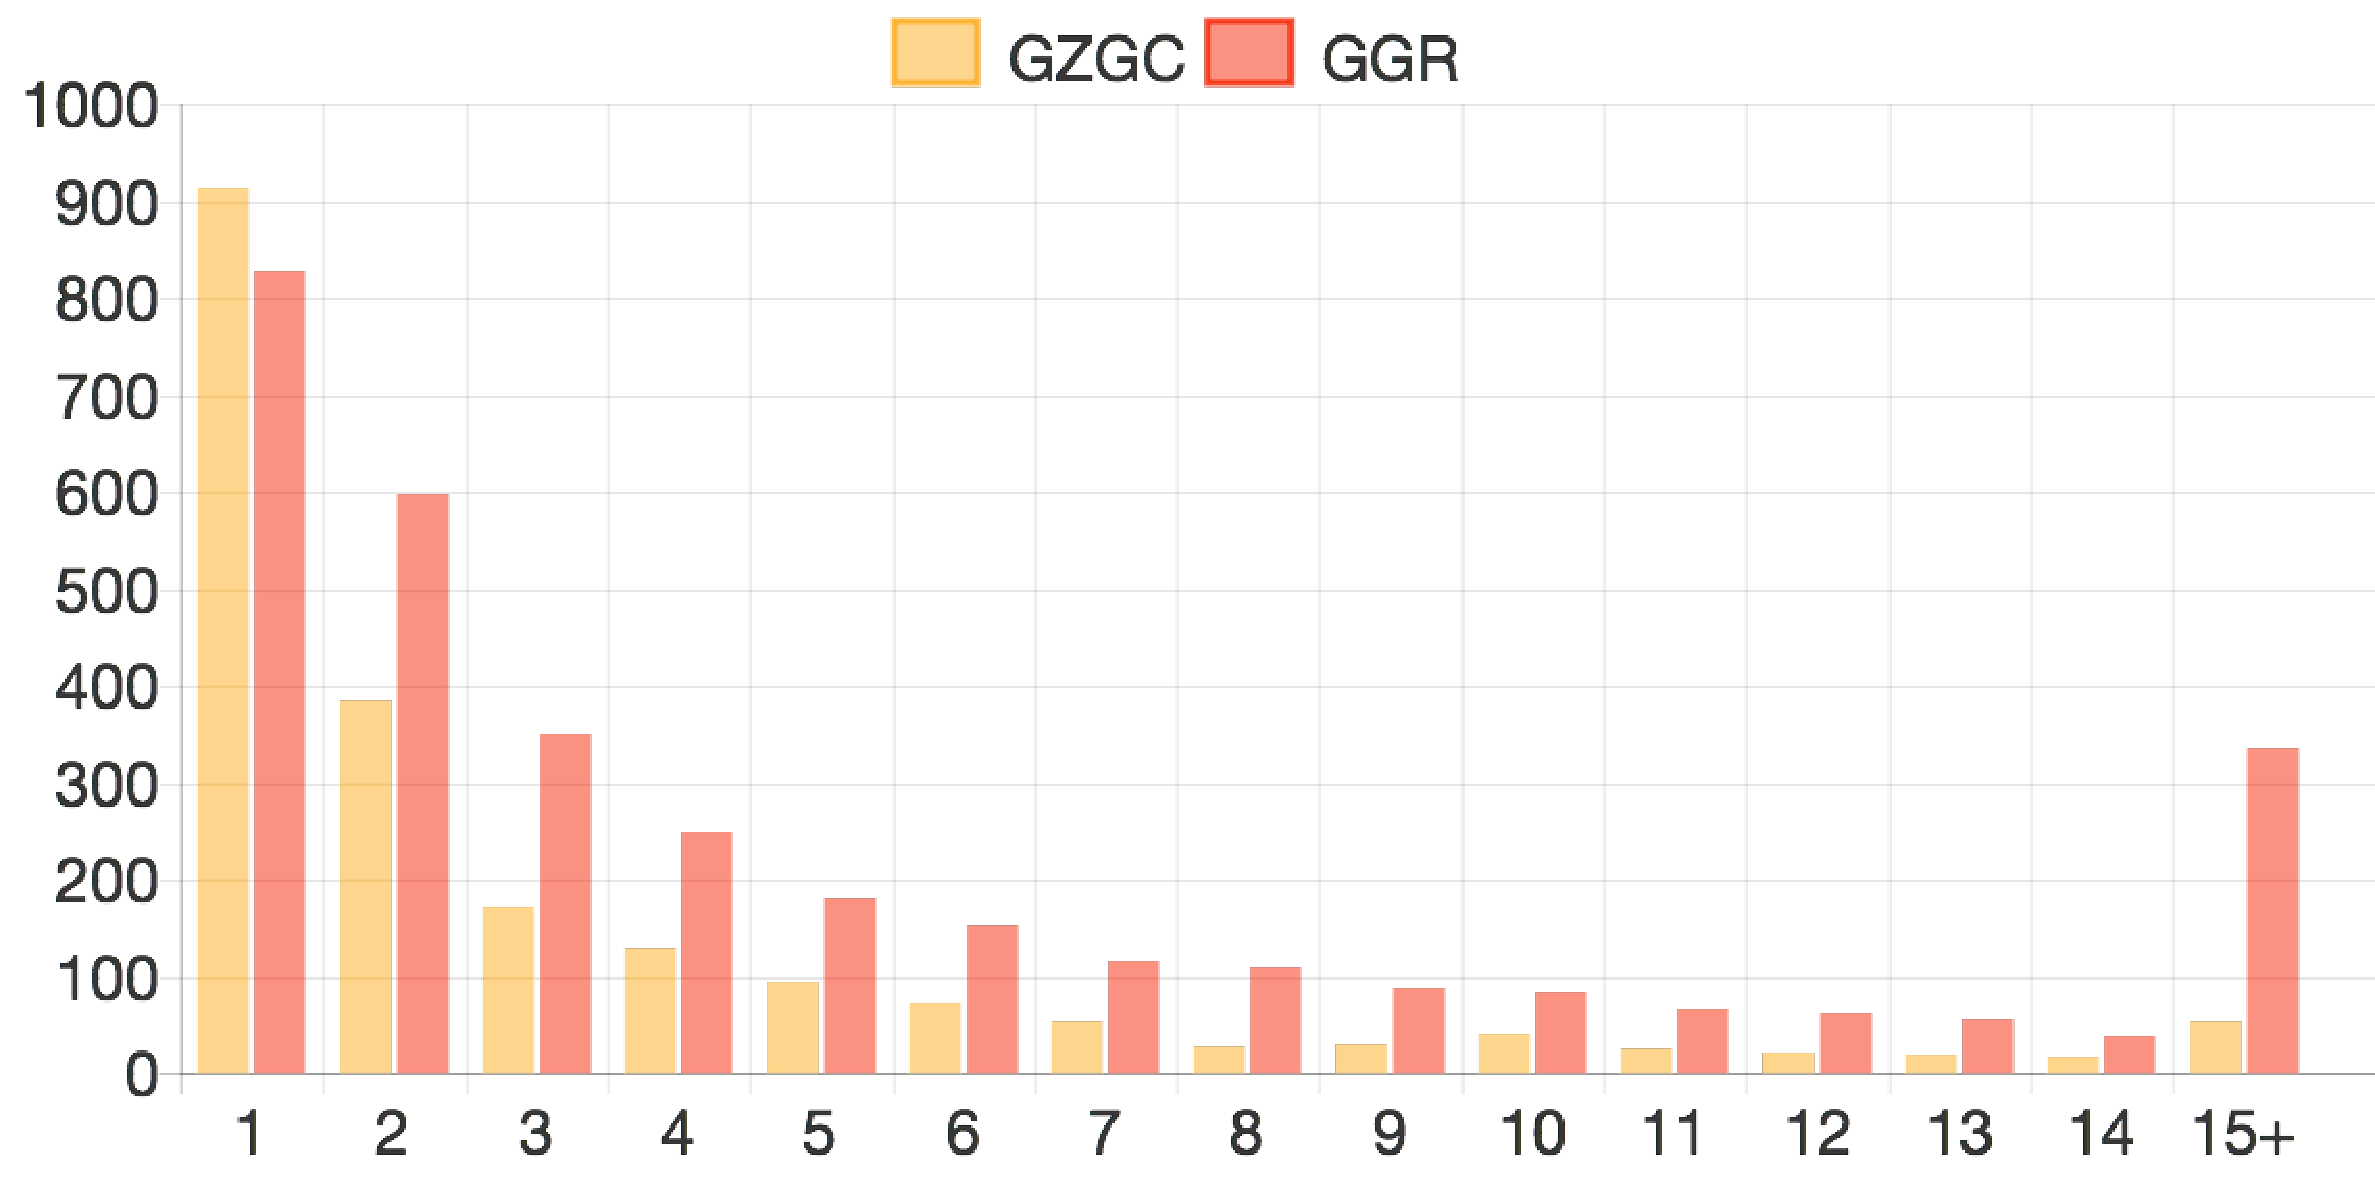
\includegraphics[width=0.8\linewidth]{resources/sightings-histogram-linear-event-15.pdf}
    \end{center}
    \caption{The number of photographers per animal ID for the GZGC and GGR-16 photographic censusing rallies.  The total number of photos from the GGR is much higher than the GZGC, and the number of 15+ photos is much more saturated, indicating better coverage and that the number of resights should be much higher.  \copyright 2017 AAAI. Reprinted, with permission, from: J. Parham, J. Crall, C. Stewart, T. Berger-Wolf, and D. I. Rubenstein, ``Animal population censusing at scale with citizen science and photographic identification,'' in \textit{AAAI Spring Symp.}, Palo Alto, CA, USA, Jan. 2017, pp. 37–44.}
    \label{fig:photographs}
\end{figure}

\begin{table}[!t]
    \caption{The number of annotations, matched individuals, and the final mark-recapture population size estimates for the three species of GZGC, GGR-16, and GGR-18.  The Lincoln-Petersen (L-P) estimates are calculated with a 95\% confidence interval.  \copyright 2017 AAAI. Reprinted, with permission, from: J. Parham, J. Crall, C. Stewart, T. Berger-Wolf, and D. I. Rubenstein, ``Animal population censusing at scale with citizen science and photographic identification,'' in \textit{AAAI Spring Symp.}, Palo Alto, CA, USA, Jan. 2017, pp. 37–44.}
    \label{table:stats}
    \begin{center}
        \begin{tabular}{| l | r | r | r |}
            \hline
            Censusing Rally    & Annotations & Individuals & L-P Estimate  \\
            \hline
            GZGC Masai         & 466         & 103         & 119$\pm$4     \\
            \hline
            GZGC Plains        & 4,545       & 1,258       & 2,307$\pm$366 \\
            \hline
            GGR-16 Gr\'evy's   & 16,866      & 1,943       & 2,269$\pm$95  \\
            \hline
            GGR-18 Gr\'evy's   & 10,044      & 1,972       & 2,812$\pm$171 \\
            \hline
            GGR-18 Reticulated & 4,018       & 992         & 2,309$\pm$332 \\
            \hline
        \end{tabular}
    \end{center}
\end{table}

Next, we turn our attention to determining how well the censusing events sampled the underlying animal population.  Figure~\ref{fig:convergence} plots the number of new animals identified vs.\ the number of processed photographs, ordered chronologically.  Ideally, these curves should flatten over time, indicating that the rate of encountering unknown individuals in the database is slowing.  The slope of the GZGC curve~\cite{parham_photographic_2015} flattens out over time but does not entirely converge.  The final GZGC slope suggests that if there were additional photographs to analyze, then new individuals were likely going to be discovered (increasing the population estimate and narrowing the confidence interval).  We can compare the GZGC curve to the GGR-16 and GGR-18 curves, which are flattening out much faster and starting to converge.  The GGR curves suggest that collecting more photographs may not have substantially impacted the final population estimate because new IDs were becoming rare.  This intuition is supported by Figure~\ref{fig:breakdown} (right), which explicitly shows a higher percentage of resights in the GGR compared to GZGC and indicates overall better coverage of the underlying population.

Figure~\ref{fig:photographs} plots a histogram of the number of photographs per animal. It shows that most frequently, an animal was photographed only once during both rallies. However, the collection protocol encouraged volunteers to take three photographs of a sighted animal, which disagrees with this histogram.  Ideally, the number of animals seen only once should be low, while the number of sightings distributed around three sightings should be abnormally elevated. Unfortunately, the actual distribution suggests that this collection request was challenging for the volunteers to follow consistently.  Encouragingly, the number of animals with single-sightings \textit{decreased} between the GZGC and the GGR-16, even though the number of annotations more than tripled.  This improvement suggests that more thorough sampling (i.e., more volunteers) and better training can help correct this bias.

\subsection{Animal Population Estimates}

At long last, the population estimates of the GGR-16 and GGR-18 on Gr\'evy's zebra and reticulated giraffes can be computed using their respective animal ID databases.  The population estimates from the GZGC~\cite{parham_photographic_2015} are also provided for Plains zebras and Masai giraffes as a comparison. In addition, Table~\ref{table:stats} provides a summary of the number of annotations used for identification, the number of sighted individuals, and the Lincoln-Petersen index as the population estimate.

\subsubsection{Results of GGR 2016 (GGR-16)}

Over 40,000 images were collected for the GGR-16, which resulted in 16,866 annotations and 1,942 animal IDs after curation was performed.  The animals sighted during the GGR-16 were sighted on either day 1 only, day 2 only, or were sighted on both days.  A total of 1,416 individuals out of 1,942 were seen on day 1, a 72.91\% sampling rate of the total population of sighted individuals.  During day 2, a slightly lower number of animals was seen at a total of 1,338, representing a percentage of 68.90\%.  The number of animals that were resighted between the two days was 835.  These statistics can be used to generate a Lincoln-Petersen population estimate, as shown in Table~\ref{table:stats} with a confidence interval of 95\%.  The population estimate of 2,269$\pm$95 indicates that during the GGR-16, between 82\% and 89\% of the surveyed population as seen.  These statistics suggest that the methodology from 2016 was mainly effective at sampling the resident populations of Gr\'evy's zebra.

Unfortunately, upon analyzing this data as broken down by county (see Table~\ref{table:stats-county}), there were abnormally low population densities in the most northern censusing blocks. In addition, these blocks had a sparse set of citizen scientists across a vast geographical area, resulting in a substandard sampling.  As a result, only 45 and 46 individuals were sighted for days 1 and 2 of the GGR-16 censusing rally, and only 26 were resighted.  These small numbers were compared to an adjoining county that found roughly 240 individuals with over 170 resighted individuals each day.  For the GGR-18, additional efforts were explicitly focused on the northern counting blocks to provide better coverage and correct the previous GGR event.

\begin{table}[!t]
    \caption{The number of annotations, matched individuals, and the final mark-recapture population size estimates for Gr\'evy's Zebra for the GGR-18, by county.  The Lincoln-Petersen (L-P) estimates are calculated with a 95\% confidence interval.  The county breakdown has a slightly lower total due to images that did not properly localize within the exact county areas yet was matched by the identification pipeline.}
    \label{table:stats-county}
    \begin{center}
        \begin{tabular}{| l | r | r |}
            \hline
            Kenyan County            & GGR-16 L-P Estimate & GGR-18 L-P Estimate \\
            \hline
            Isiolo                   & 299$\pm$54          & 597$\pm$182         \\
            \hline
            Laikipia                 & 1199$\pm$59         & 1328$\pm$105        \\
            \hline
            Marsabit                 & 66$\pm$17           & 250$\pm$166         \\
            \hline
            Meru                     & 344$\pm$30          & 384$\pm$36          \\
            \hline
            Samburu                  & 452$\pm$80          & 642$\pm$172         \\
            \hline
            \hline
            \textit{Northern Blocks} & 80$\pm$21           & 545$\pm$265         \\
            \hline
        \end{tabular}
    \end{center}
\end{table}

\subsubsection{Results of GGR 2018 (GGR-18)} \label{sec:ggr-results}

The number of participating photographers increased by 33\% during the GGR-18 censusing event.  The photographers contributed over 49,000 images, representing a 21\% increase compared to the GGR-16 event.  The increased number of collected photographs was due to adding more photographers and including reticulated giraffes as a second species of interest.  More than 23,000 images contained the primary species of Gr\'evy's zebra, whereas over 18,000 images contained sightings of reticulated giraffes.  These images resulted in 10,044 annotations that were used for identification for Gr\'evy's and 4,018 for giraffes.  The drop in identifiable annotations between the GGR-16 and GGR-18 for Gr\'evy's zebra can be explained by more a restrictive filtering process within the detection pipeline.  This filtering drastically reduced the overall number of human reviews required by the identification pipeline but slightly increased the population estimate error bounds compared to the GGR-16.  Within those annotations, a total of 1,972 unique Gr\'evy's zebra and 992 unique reticulated giraffes were sighted.

A total of 1,251 individuals out of 1,972 zebras were seen on day 1, a 63\% sampling rate of the total population of sighted individuals.  During day 2, a slightly higher number of zebras was seen at 1,299, representing a percentage of 65.9\%.  It is worth noting that these sampling numbers are relatively consistent with the GGR-16 sampling.  For the GGR-18, the number of zebras that were resighted between the two days was 578.  This value is much lower, suggesting that either the population has gotten significantly larger (unlikely), the sampling procedure was not thorough enough (a constant issue), or the detection pipeline was slightly too restrictive.

The population estimate of 2,812$\pm$171 for zebras indicates that, during the GGR-18, somewhere between 66\% and 75\% of the surveyed population was seen.  Again, these numbers are lower than the GGR-16, possibly indicating a step backward in sampling or the quality of images.  These statistics suggest that our methodology from 2018 was still effective at sampling the resident populations of Gr\'evy's zebra, but not as thorough as the 2016 census. However, the analysis is not entirely bad news when looking at county breakdowns of the GGR-16 and GGR-18 census estimates, as shown in Figure~\ref{table:stats-county}.  The northern blocks were sampled much more heavily during the GGR-18, and an estimated 400 animals were recovered due to better sampling.  The county breakdowns of southern counties with the largest populations (Laikipia, Samburu, and Meru) as their population estimates are stable, providing a measure of confidence in the methods used.  The error bounds for these counties are also overlapping, suggesting that any bias in the population estimate is not statistically significant for the vast majority of the animals.

For giraffes, on day 1, 613 individuals were sighted, 516 on day 2, and 137 were resighted across both days.  These numbers are much smaller, and the sampling ratios are much smaller.  The drastically smaller resighting value compared to the total number of individuals is reflected by a high estimate (and error bound) for the giraffe population.  The statistics suggest that the number of giraffes in the surveyed population area is 2,309$\pm$332.  The giraffe results are to be treated as tentative, pending a re-censusing in 2020.

\section{Culminating Experiment on GGR 2018} \label{sec:ggr18-culminating}

This section sets aside the narrative tone from the above discussion on the GGR and how its results were calculated. Instead, the purpose of this culminating experiment is to provide a condensed walk-through of the most current, recommended process for animal photographic censusing in 2021.  As such, we can opt to rely on the pre-trained detection pipeline and advanced Census Annotation machine learning models that have been introduced.  What follows is an end-to-end analysis by following the steps listed in Figure~\ref{fig:gantt} (starting just after the ``Image Aggregation'' step) on a large animal population.

The population estimates from the GGR-16 and GGR-18 were a product of their respective times and the states of the computer vision algorithms available to them.  The field of computer vision has advanced drastically between then and now, with some of the components introduced in this thesis not even being available at the time of their original analysis.  However, to demonstrate the effectiveness of concepts like Census Annotations and the LCA curation algorithm, we wish to audit a GGR censusing event with modern tools.  The benefit of having photographic ID evidence for a population is that newer machine learning approaches can be evaluated for improvements in accuracy and human involvement.  This section performs a new, standalone analysis of the data collected by the GGR-18 photographic censusing event (only for Gr\'evy's zebra) and compares the population estimates to the values reported in Section~\ref{sec:ggr-results}.  This analysis focuses on the GGR-18 over the GGR-16 event because it is the most representative geographic sampling (covering the northern blocks) and is the active population estimate provided by the Kenyan government.

We processed all of the raw GGR-18 imagery fresh for an end-to-end run-through of the entire procedure.  We imported a total of 56,588 valid images and ran the automated detector pipeline on the images.  The localizer was configured using the pre-trained GGR-18 Gr\'evy's zebra model and used an NMS threshold of 40\% and an operating point of 40\%.  The localization model produced 104,858 annotations, with 73,356 of those labeled with the generic \texttt{zebra} label.  Using a single NVIDIA Titan RTX and a 20-core server, the bounding box regression computation took approximately 6.5 hours.

The GGR-18 census event asked volunteers to take right-side shots of Gr\'evy's zebra, so we need to use the labeler network to filter out other species (including plains zebra) and any viewpoints that did not show the right side.  The labeler was trained using a collection of Gr\'evy's and Plains zebra data and various viewpoints.  The \texttt{zebra\_v1} model (an ensemble of DenseNet-style neural networks) was configured such that the most confident \texttt{species:viewpoint} prediction that was returned was used as the final label.  The labeler computed results on the same accelerator hardware in approximately 5.5 hours.  The labeler produced a classification of \texttt{zebra\_grevys} for 67,409 annotations, but approximately half of those showed the incorrect viewpoint.  The algorithm predicted 23,458 ``right'', 8,735 ``front-right'', and 8,273 ``back-right'' viewpoints labels; all annotations that were not Gr\'evy's zebra or that did not show the right side were discarded, leaving 37,199 for further processing.  These annotations were sourced from 20,015 original images.

Next, the \texttt{V4} CA classifier (see Section~\ref{sec:ca}) was run on these images to identify the most likely Census Annotations for ID.  The inference ran for 1 hour and 40 minutes and produced a set of 15,072 Census Annotations (threshold = 0.31).  For reference, using a CA classifier threshold of 0.1 results in 16,848 annotations while using 0.9 ends with 11,381. Thus, using the recommended threshold of 0.31 keeps the majority of the borderline CAs. Next, each CA was passed to the CA Region regression network, which took 42 minutes to compute.  Once the bounding boxes were generated, we performed NMS (IoU = 1.0) to prevent overlapping CA Regions by suppressing the lower-scoring box as determined by the CA classifier.  The purpose of using an IoU of 100\% was to guarantee zero overlap between annotations within an image, drastically reducing the incidence rate of mother-foal photobombs.  This filtering resulted in 14,742 Census Annotation Regions for right-side Gr\'evy's zebras; these annotations were sourced from 12,772 images, indicating a utility rate of the citizen science capture of 22.6\%.

Next, we synchronized all of the GPS locations and timestamps for all of the images (and source cameras) for these Census Annotation Regions.  All annotations taken outside the GGR-18 date range (Day 1: 1/27/2018 and Day 2: 1/28/2018) were discarded.  The standard GPS synchronization step was delayed until now to focus on only the images that contributed useful Census Annotation Regions.  There were 7,737 annotations taken on Day 1 and 6,116 on Day 2, coming from 11,991 images.  Additional filtering eliminated poor qualities based on pixel size, aspect ratio, and gradient magnitudes (blurriness).  While the CA classifier does an excellent job filtering out incomparable sightings, it still makes some mistakes.  Most of the CA classifier's mistakes come from blurry annotations, and -- while they are subjectively challenging pairs and take humans a long time to decide -- they are comparable.  The average aspect ratio (height / width) was calculated and any box outside of 2.0 standard deviations was discarded (min = 0.328, max = 1.449, mean = 0.612, std = 0.109), removing 698 annotations.  A similar filter was applied to the total number of width and height pixels for each annotation.  An additional 281 annotations were removed (minimum width 245 pixels, minimum height 161 pixels) using a minimum threshold of the mean minus 1.5 standard deviations.  Lastly, we computed the average gradient magnitude across the image using an x-axis and y-axis Sobel filter (kernel size 3).  The average of the gradient magnitude mean for all annotations was calculated as 86.0 on \texttt{uint8} RGB 3-channel cropped chip with a maximum-linear dimension of 700 pixels (min = 12.8, max = 182.5, mean = 86.0, std = 27.9).  All annotations with a mean gradient less than 1.5 standard deviations under the average mean gradient (less than 44.2) were removed.  This left 11,916 annotations (Day 1: 6,677, Day 2: 5,239) and 10,558 images.  All other annotations and images that did not contain a Census Annotation Region or passed these photometric quality filters were discarded and not used for further analysis.  All processing up to this point has been completely automated.

Next, the LCA algorithm was initialized by loading a pre-trained weighter function.  The weighter was created from 500 positive and 500 negative pair decisions from the GZCD dataset (see Section~\ref{sec:gzcd}).  Next, the match candidates were sampled using a HotSpotter rank list for all of the CA Regions (tuned for $K=5$, $K_{\text{norm}}=5$, $n_{\text{top}}=10$, spatial verification was ON, scoring method \textit{csum}) that found 67,247 pairs.  The VAMP model trained on Gr\'evy's zebra CA Regions was used as the verification algorithm and applied to all matching pairs.  In total, 13,848 negative weights, 10 neutral weights, and 53,389 positive weights were found by the VAMP verifier for LCA.  The LCA algorithm then proceeded to try alternative pairs of clusters, asking for VAMP and human decisions, as it worked.  The pairs that the algorithm wanted a human decision were given to a web interface and reviewed by the author.

In total, it took just under 12 hours for the LCA algorithm, working with a single human reviewer to converge.  The LCA process attempted 23,783 alternative clusterings and requested an additional 19,160 VAMP decisions during its automated processing.  The ID curation process required just 1,297 human decisions before converging.  For reference, the original GGR-18 analysis using the Graph ID algorithm required 18,556 human decisions.  The resulting ID database was then checked to ensure no erroneous IDs with poor singletons needed to be excluded (i.e., the detection pipeline failed to filter them out).  In total, 15 IDs were excluded for having too poor quality, leaving 2,022 unique IDs in the database.  The demographics labeling step was skipped, and the gender checks were not performed for the sake of a more straightforward verification, but the speed check resulted in zero IDs being marked for review.  A total of 1,338 individuals were seen on day 1, 1,326 animals were seen on day 2, and 642 animals were seen on both days. The final Lincoln-Petersen estimate using this new ID database was 2,764$\pm$154, consistent within 1.7\% with the reported estimate on GGR-18 (2,812$\pm$171).  Furthermore, this result was 93\% less human effort than the GGR-18 processing and was completed with the effort of a single working day for one person.

Finally, we need to incorporate the estimated machine learning loss terms from Equation~\eqref{eq:final} (in Chapter~\ref{chapter:overview}) into the final population estimate.  Recall that the equation has been modified to accept three new terms $\hat{p}_{mm}(\theta)$, $\hat{p}_{ms}(\theta)$, and $\hat{p}_{dm}(\theta)$.  The term $\hat{p}_{ds}(\theta)$ is assumed to be zero as each of the final singletons were manually checked for quality.  Furthermore, using Census Annotation Regions helped to reduce the rate of photobombs and scenery matches drastically.  The LCA algorithm was also configured to do an additional brute-force check for potential incidental matches, ensuring that each name cluster had more stability with extra automated checks beyond what was requested by the ranking algorithm.  The verification allows us to make the assumption that $\hat{p}_{ms}(\theta)$ is also close to zero, leaving $\hat{p}_{mm}(\theta)$ and $\hat{p}_{dm}(\theta)$ as the primary terms to impact the result.  The reported GGR detection recall performance on AoI Gr\'evy's zebra is 96\%, indicating that ~4\% of the annotations are missed.  Furthermore, the CA classifier has a false-negative rate of 1.8\% on the GZGC dataset, so a conservative detection miss rate of 6\% is estimated for $\hat{p}_{dm}(\theta)$.  For $\hat{p}_{mm}(\theta)$, the top-10 recall rate for HotSpotter on Gr\'evy's zebra CA-Rs in the GZCD is 99.2\%.  We must also consider the VAMP failure rate for CA-R \texttt{match} decisions of 1.4\%.  These effects combined, but with the human verification of borderline matches, give us a conservative estimate for $\hat{p}_{mm}(\theta)$ at 2\%.  Using these values suggests a correction value of +56 IDs for the population estimate and a widening of $\pm$13 for the confidence interval.  The final corrected population estimate with high degrees of automation is therefore 2,820$\pm$167 (0.3\% off), compared to the originally reported estimate for GGR-18 of 2,812$\pm$171.  Furthermore, the original GGR-18 analysis marshaled dozens of participants and took around three months to complete.  In sharp contrast, the new analysis took approximately two days -- with the majority of that time dedicated to hands-off, automated computing -- and only relied on one person.

\section{Summary}

The Great Gr\'evy's Rally (GGR) is the most extensive photographic census of the Gr\'evy's zebra species ever performed in Kenya.  The country of Kenya is the primary residence of Gr\'evy's zebra, indicating that the population estimates from the GGR are also comprehensive for this critically endangered species.  Furthermore, the data collection rallies in 2016 and 2018 are a real-world demonstration of the principles of citizen science and the benefits of using volunteer photographers in data collection.  Across the GZGC and GGR censusing rallies, over 100,000 photographs were processed and collected by more than 400 volunteer citizen scientists (90,000+ images and 350+ volunteers for GGR alone).  Furthermore, the GGR-16 and GGR-18 rally procedures were significantly improved by increasing the automation of the detection and identification processing, streamlining data collection with GPS-enabled cameras, and proving that the original methodology from the GZGC scales to thousands of animals.  Unfortunately, even though the data analysis for GGR-18 was done with automated tools, it still required large amounts of work (nearly 20,000 human decisions), cost USD \$50,000+, and took over three months.

Luckily, new advances to the ID curation process since the conclusion of GGR-18 have been developed: Census Annotations, Census Annotation Regions, the LCA curation algorithm, and a new Lincoln-Petersen index estimator.  The primary motivation of these components is to increase the automation of photographic censusing further and reduce the known issues (e.g., incidental matching) that were encountered during the GGR-16 and GGR-18 analysis.  As a result, these new methodologies were used to reprocess the original GGR-18 collection from scratch.  In total, 56,588 images were automatically processed by the pre-trained detection pipeline, and 11,916 annotations were found for comparable, right-side Gr\'evy's zebra.  The ID curation process required 1,297 human decisions before converging and estimated 2,764$\pm$154 Gr\'evy's zebra in the population.  After modifying for various known ML errors, the estimate was updated to 2,820$\pm$167.  This result is consistent (within 0.3\%) with previous estimates on GGR 2018 data and was achieved with a 93\% reduction in human effort.  This new automated image analysis procedure will be employed on the newly collected data for GGR in 2020 (GGR-20) and beyond.

In summary, the GGR-18 censusing rally produced a population estimate of 2,812$\pm$171 for Gr\'evy's zebra, indicating approximately 70\% of the population has been included in the ID census database.  Furthermore, the 2018 population of reticulated giraffes in Kenya is estimated to be 2,309$\pm$332.  These estimates are consistent with previous sampling counts and provide a new image-based ID database for historical trends.

\subsection{Lessons Learned}

Having completed three successful events, having developed both logistic support methods for running the events, and having new computer vision/machine learning algorithms for analyzing the resulting image data, we conclude this chapter with a discussion of lessons learned about applying photographic censusing in the real world.  For example, the prototype photographic censusing event, the Great Zebra \& Giraffe Count (GZGC)~\cite{parham_photographic_2015}, was marred by metadata synchronization issues (no GPS-enabled cameras), an inability to eliminate problematic annotations (no CA for incidental matching), relied exclusively on human decision making for detections (no pre-trained models) and pairwise review (no VAMP), had no concept of ID curation or consistency checks (no Graph ID or LCA), did not know beforehand how helpful citizen scientists were going to be at image collection (no established baseline), and took three months of hand-crafted analysis (no existing tooling or software).  These problems translate directly into a high logistical burden on conservation administrators and, if left unaddressed, would undercut photographic censusing as an attractive alternative to more invasive monitoring methods.

Since our initial start in 2015, however, the methodology for photographic censusing has dramatically improved.  The lessons that have been learned have translated directly into a proven, end-to-end system that the Kenyan government is actively using to track animal populations.  The challenges encountered during the GZGC, the GGR-16, and the GGR-18 -- emphasizing that some were significant barriers -- offered a guiding framework for designing a more robust, reliable, verifiable, automated, sustainable, and repeatable methodology.  With the conclusion of this chapter, let us review some of the most influential takeaways and high-level recommendations from this concerted and sustained research effort:

\begin{itemize}
    \item \textbf{Citizen Science} - the completed photographic censusing events have demonstrated that distributing data collection for specific ecological research is highly effective.  Furthermore, incorporating volunteers is a natural way to engage with a local community with science projects.  When required, any training procedures should focus on being easy-to-understand and, ideally, should fit onto a single page.  The presented research has shown that citizen scientists can quickly learn and conform to specific and focused data collection goals.
    \item \textbf{On-the-Ground Participation} - there is little substitute when performing a photographic census for on-the-ground participation of the principal investigators.  The nuances of distributed data collection are hard to predict and may significantly impact the effectiveness of the overall event.  Furthermore, participating in the photographic census in-person allows for engagements with conservancy managers, park rangers, and field ecologists, who may be mandated by law to maintain accurate population estimates.  Establishing relationships with these science brokers is crucial because it 1) allows for an accurate assessment of the correct geographical coverage area to capture the known range for the species of interest and 2) provides a touch-point for setting up a routine and secure exchange of the latest ecological data as it is collected.  Lastly, engaging with local data brokers and policymakers helps prevent claims of ``exporting'' the data from the conservation area, depriving a local entity of their sense of agency and self-determination in conservation action.  Furthermore, establishing productive partnerships with ecologists is an ethical and sustainable way to collect animal data for ML research.
    \item \textbf{Local Infrastructure} - it is essential to consider and be aware of the local infrastructure (e.g., power, internet, cell service) and its limitations during a photographic censusing event.  Dispatching photographers into remote areas may have inherent safety concerns, and the final aggregation of the collected data should be based on a reliable mechanism.  For example, having intermittent access to stable power may prioritize battery-powered laptops for the event administrators.  Likewise, ecology research for endangered species can be performed in areas without reliable or fast access to the Internet.  This limitation means that communication with cloud-based servers may not be available, and the ML processing must be delayed or done locally with power-hungry, high-performance GPUs.
    \item \textbf{Ease of Participation} - it should be easy for a volunteer to participate, with minimal requirements on the camera hardware.  The only significant restriction for proper synchronization is having at least one GPS-enabled camera within a party of photographers.  This requirement could be satisfied with a smartphone and, ideally, precludes the need for specialized camera trap hardware, access to planes, or other complications like veterinary licensing. In addition, a detailed aggregation and synchronization plan should be established prior to the data collection event.  Furthermore, this plan should include details on properly cleaning, sanitizing, and discarding inappropriate images that may be accidentally contributed.  Lastly, using registration cards allows for large numbers of participants to contribute data with minimal record-keeping and the need for real-time coordination.
    \item \textbf{Ease of Scale} - a photographic census is designed to have a fixed geographic area sampled on two consecutive days.  The participation of photographers should be structured such that minimal to no coordination is required between photographers. For example, large sampling areas can be broken up into zones to ensure uniform coverage. Increasing the sampling density for a given area simply requires assigning more participants.  After the two days of the event, all of the image data will need to be physically collected at a centralized location or otherwise submitted to the administrators for aggregation.
    \item \textbf{Open Populations} - photographic censusing is designed for open animal populations where the actual number of individuals is not known.  While censusing open populations means a formal validation of the results is not possible, the methodology has produced results consistent with historical estimates for multiple species in Kenya.  Furthermore, no inherent limitation would make photographic censusing incompatible with closed populations for more precise evaluations.
    \item \textbf{Data Wrangling} - after collecting the image data from photographers, there has always been a non-trivial step of cleaning, organizing, and otherwise preparing the raw data for machine learning processing.  This process is typically done manually (e.g., copying images off an SD card into a folder) and is subject to human errors and poor standardization.  The aggregated imagery might also require large amounts of storage, and the logistics of transferring and backing up the entire censusing event should be considered carefully.  Another challenge is when photographers forget to take their synchronization image, requiring a manual process to establish the internal time for that participant's camera.  In some instances, this synchronization can only occur after the animal IDs have been fully assigned.  A camera's time offset can be approximated by triangulating the speed consistency checks across multiple animals.
    \item \textbf{Bootstrapable Machine Learning Components} - the machine learning components that are used throughout the process are meant to be bootstrapable (i.e., trainable from scratch without access to an appropriate pre-trained model). Thus, all detection pipeline components can be trained with relatively small labor (estimated to be approximately 1,000-2,000 hand-annotated images) and do not require a fully segmented ground-truth.  In practice, a small team (1-5 people) of reviewers can gather all of the required detection ground-truth data in about a day.  Furthermore, it is recommended to implement web-based tools for multiple workers to contribute ground-truth data simultaneously.
    \item \textbf{Animal Detection} - the detection pipeline components, Census Annotations, and Census Annotation Regions all function as a way to automate the conversion of raw collected imagery to relevant annotations.  The task of ``animal detection'' as a high-level process functions as an aggressive filter and only allows easily identifiable and comparable annotations to be considered by the ID curation process.  The proposed detection components in this dissertation are designed to be modular and standalone, allowing them to be replaced without needing to modify other components in the pipeline.  These components do not need to achieve state-of-the-art performance on their respective tasks because their primary goal is to reduce work.  For example, the task-specific goal for bounding box regression is to reduce the L2 regression error, but there is an overriding goal to decrease the incidence rate of incidental matching. Furthermore, we do not need the best and most up-to-date detectors computer vision offers to calculate an accurate population estimate.  Lastly, not all detections are equally important (i.e., missing a blurry background animal is not an error), and the detection components should be optimized for the specific purpose of filtering out incompatible, unidentifiable, incomparable, or otherwise problematic annotations.
    \item \textbf{Human Verification} - a critical determination for a new candidate species is if a human can accurately and timely tell if two annotations show the same individual or not.  For example, performing a photographic census on the common American red squirrel is likely not very productive because people have a hard time telling two squirrels apart.  As such, the utility and accuracy of any photographic census are explicitly tied to how accurately a human can correctly verify potential matched pairs.
    \item \textbf{Continual Curation} - selecting which curation algorithm to use is vital, as its implementation details can significantly influence automation. For example, the Graph ID algorithm~\cite{crall_identifying_2017} was found to be too rigid, too iterative, and too quick to explicitly enforce consistency, leading to the need for many thousands of additional reviews.  Alternatively, the LCA algorithm is more appropriate for photographic censusing because it allows for qualitative decisions that do not block the processing workflow, which dramatically reduces the need for human effort while maintaining accuracy.  Furthermore, a photographic census produces a consistent and highly-reliable database of animal IDs but may start from different underlying database states.  For example, a photographic census may be started with an empty database, a sizeable pre-existing database that has already been thoroughly curated, or a pre-existing database with many unresolved issues (i.e., merges, splits, consistency checks).  The ID curation algorithm must be capable of handling these different starting conditions.
    \item \textbf{Bootstrapable ID Databases} - large-scale animal ID databases are rare, and photographic censusing is an end-to-end process that facilitates the creation of large, highly-consistent databases for animal ID research.  Furthermore, some of the newest and most accurate machine learning approaches for re-identification (i.e., triplet loss) need to be trained on an existing database of IDs.  This limitation means that approaches that do not rely on deep learning (e.g., HotSpotter~\cite{crall_hotspotter_2013}, VAMP~\cite{crall_identifying_2017}, CurvRank~\cite{weideman_integral_2017}, and even Graph ID~\cite{crall_identifying_2017}) are required to enable starting an ID database from scratch.  Once a critical mass of IDs has been gathered, these tools can be replaced for more advanced and accurate approaches like PIE~\cite{moskvyak_robust_2019}.  Lastly, from experience, it is important not to underestimate the time and challenge it will take to collect and curate reliable animal ID data for computer vision research.
    \item \textbf{Reporting ID Ranking Performance} - there is often a disconnect with how animal ID ranking performance is standardized and reported.  For example, it is crucial to consider the underlying distribution for the number of annotations per name, the percentage of singletons in the database, and the time between sightings.  As a general rule of thumb, it is recommended that ID ranking and recall performance be reported as the average percentage for all annotations in a database for top-1, top-5, top-k.  Any experimental evaluation should start by defining a fixed set of annotations where each animal ID has a minimum of 2 annotations, a maximum of 5 annotations, and a minimum of 24 hours between any pair of its annotations.  This structure guarantees that 1) there is always a correct answer to be found in the top-1 rank, 2) that an over-sampled name does not improperly skew the reported recall performance, and 3) that trivial matches separated by seconds or minutes are removed.  Furthermore, the performance should be reported as the average across all annotations (i.e., annotation recall) and all names (i.e., name recall).
    \item \textbf{Ownership \& Security of Animal IDs} - it is essential to consider the ethics of claiming ownership of an animal's identification.  There is an inherent obligation to protect an endangered species when performing an ecology study. It includes being responsible for how sensitive metadata is accessed and requires a willingness to embrace collaboration opportunities with other researchers.  For example, it would be unethical for a researcher to claim exclusive ownership of an animal's ID to the detriment of more effective conservation action and insight.  Stated simply: a wild animal's ID does not belong to you, it belongs to the animal that is facing extinction.  Likewise, careful consideration for sensitive metadata (e.g., GPS locations, timestamps) should be paid for poached and critically endangered species, as a comprehensive ID database is a phenomenal surveillance tool for bad actors. A photographic census administrator's responsibility is to adequately safeguard any sensitive information to protect the life, health, and unique identity of any endangered animal.
    \item \textbf{Extensibility \& Sustainability} - the real-world reality of photographic censusing is that it is currently a highly-specialized endeavor, dependent on advanced computer science and computer vision expertise.  Therefore, it is imperative to consider hosting all code under a permissive open-source license and with a freely available repository service. In addition, the publication of free pre-trained models offers an opportunity for collaboration and reproducing results.  Lastly, the financial reality of machine learning-powered ecology is currently dependent on support from governments, NGOs, not-for-profits, private industry grants, and philanthropic foundations. For example, this dissertation focuses heavily on just a single species (Gr\'evy's zebra) because it takes so much time, energy, and money to collect and curate good ID datasets like the GZCD.  Therefore, the lack of a mature, self-sustaining, open-source community for automated wildlife monitoring represents a substantial existential crisis for the long-term adoption of photographic censusing.
\end{itemize}

\noindent In conclusion, this dissertation proposes a new paradigm for animal population monitoring; the high level of accuracy and automation that has been demonstrated will ideally transform ecology into a data-driven science.
